\documentclass[acmsmall,review,anonymous,nonacm]{acmart}
\usepackage{mathpartir}
\usepackage{cleveref}
\usepackage{listings}
\usepackage{svg}
\usepackage{float}
\usepackage{caption}
\usepackage{subcaption}
\usepackage{graphicx}
\usepackage{amsmath}
\usepackage{multirow} 
\usepackage{tikz}
\usepackage{listings}
\usepackage{xcolor}
\usepackage{booktabs} 
\usepackage{arydshln}
\usepackage[table]{xcolor}
\usepackage[dvipsnames]{xcolor}  
\usepackage{siunitx}
\usepackage{multirow}
\usepackage{pifont}
\usepackage{calc} 
%\newcommand{\cmark}{\textcolor{green}{\ding{51}}}
\usepackage{wrapfig}             % for wrapfigure
\usepackage[export]{adjustbox}   % for trim/clip keys on includegraphics
\usepackage[T1]{fontenc}
\usepackage{tcolorbox}           % for colored boxes
\newcommand{\cmark}{\checkmark}
%\definecolor{brightbrown}{RGB}{245,237,205}%{205,133,63}
%\colorlet{darksand}{Tan!50!black}
%\definecolor{strongyellow}{RGB}{255,220,0}
\definecolor{brightyellow}{RGB}{255,247,192}%{255,255,102}
\definecolor{lightchacki}{RGB}{245,237,205}%{235,220,187}
\usepackage{mathtools,amssymb,mathpartir}

% ---- handy notation (optional) ----
\newcommand{\cfg}[3]{\langle #1,\; #2,\; #3\rangle}
\newcommand{\update}[3]{#1[#2 \mapsto #3]}
\newcommand{\step}{\mathrel{\rightarrow}}
\newcommand{\pstep}{\mathrel{\Rightarrow}}


% Define darkorange via RGB or HTML:
\definecolor{darkorange}{RGB}{255,140,0}

\newcommand{\xmark}{\textcolor{red}{\ding{55}}}
\usetikzlibrary{shapes.geometric,positioning,arrows} 
\definecolor{headerbg}{RGB}{220,230,241}

\newcommand{\Pre}{\mathit{Pre}}
\newcommand{\Post}{\mathit{Post}}

% ----- Macros -----

% Tool name macro (styled like typical POPL papers)
\newcommand{\toolname}{\textsc{Ser}}

\newcommand{\guy}[1]{\textcolor{green!50!black}{G: #1}}
\newcommand{\jules}[1]{\textcolor{red!50!black}{J: #1}}
\newcommand{\markb}[1]{\textcolor{blue!50!black}{M: #1}}
\newcommand{\todo}[1]{\textcolor{gray}{TODO: #1}}


\newcommand{\grammartag}[1]{\qquad\qquad\emph{(#1)}}


% Define macros for keywords
\newcommand{\kw}[1]{\textbf{#1}}
\newcommand{\nondet}{\kw{?}}
\newcommand{\ifkw}{\kw{if}}
\newcommand{\elsekw}{\kw{else}}
\newcommand{\whilekw}{\kw{while}}
\newcommand{\yieldkw}{\kw{yield}}
\newcommand{\requestkw}{\kw{request}}

\newcommand{\sat}{\texttt{SAT}}
\newcommand{\unsat}{\texttt{UNSAT}}

\newcommand{\Parikh}{\mathsf{Parikh}}

\newcommand{\greencmark}{\textcolor{green}{\ding{51}}}

\lstdefinelanguage{CustomPseudoCode}{
	morekeywords={request, yield, return, if, else, while, and, or},
	morecomment=[l]{//},
	morestring=[b]",
	sensitive=true
}

\lstset{
	language=CustomPseudoCode,
	basicstyle=\ttfamily\small,
	keywordstyle=\color{blue}\bfseries,
	commentstyle=\color{gray}\itshape,
	stringstyle=\color{orange},
	numbers=left,
	numberstyle=\tiny,
	stepnumber=1,
	numbersep=5pt,
	backgroundcolor=\color{white},
	frame=single,
	rulecolor=\color{black},
	tabsize=2,
	captionpos=b,
	breaklines=true,
	breakatwhitespace=false,
	showstringspaces=false,
	escapeinside={(*@}{@*)},  % used for coloring "?" below
}


% ----- Main paper -----

\title{When One Message Tells the Whole Story:\\ Deciding Serializability in Network Systems}
\author{Author Name}
\affiliation{
  \institution{Institution Name}
  \city{City}
  \state{State}
  \country{Country}
}
\email{author@institution.edu}

\settopmatter{printfolios=false,printccs=false,printacmref=false}
\renewcommand\footnotetextcopyrightpermission[1]{} % removes footnote with DOI
% \renewcommand{\keywords}[1]{}  % removes "Additional keywords and phrases"
% \renewcommand{\acmSubmissionID}[1]{} % removes SUBMISSION ID
\let\oldmaketitle\maketitle
\renewcommand{\maketitle}{
  \oldmaketitle
  \pagestyle{plain}  % empty headers and footers on all pages
  \thispagestyle{plain}  % empty header and footer on the first page
}

% Make paragraph headings bold
\makeatletter
\renewcommand\paragraph{\@startsection{paragraph}{4}{\z@}%
  {1.5ex \@plus1ex \@minus.2ex}%
  {-1em}%
  {\normalfont\normalsize\bfseries}}
\makeatother

% Redefine sections to display with § symbol
\crefformat{section}{\S#2#1#3}
\Crefformat{section}{\S#2#1#3}

% Ensure subsections/subsubsections behave the same way (optional)
\crefformat{subsection}{\S#2#1#3}
\Crefformat{subsection}{\S#2#1#3}
\crefformat{subsubsection}{\S#2#1#3}
\Crefformat{subsubsection}{\S#2#1#3}

% 1) create a new length
\newlength{\subfigheight}

% 2) measure the height of (d) once the document begins
\AtBeginDocument{%
	\settoheight{\subfigheight}{%
		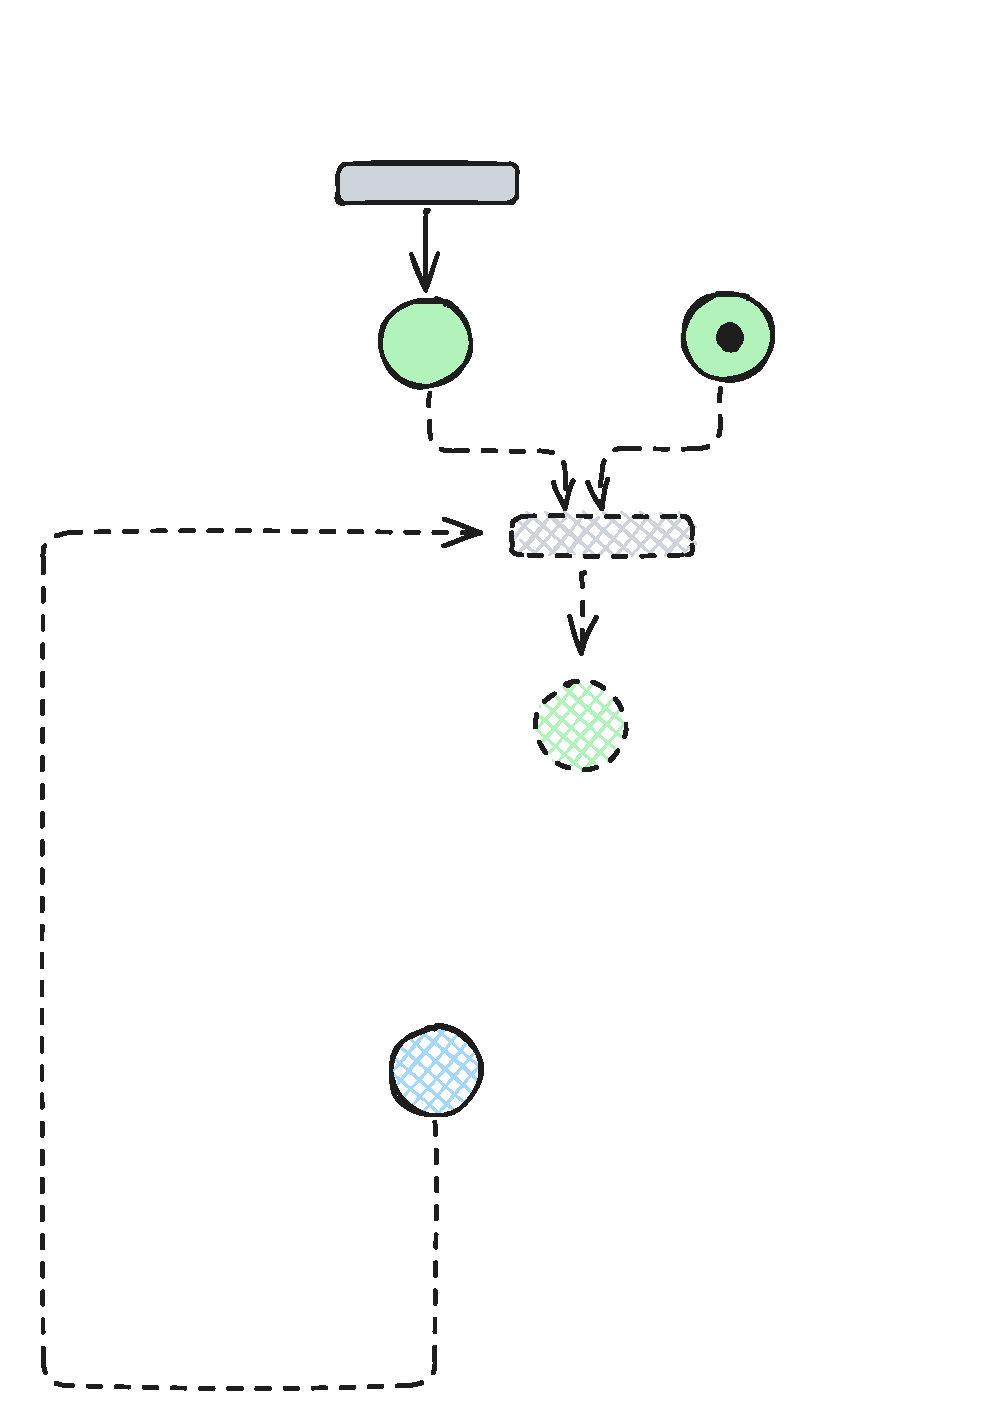
\includegraphics[width=0.23\textwidth]{plots/bidirectional_pruning_step_d_updated_2.pdf}%
	}%
}

\begin{document}

\begin{abstract}
	We introduce the \toolname{} modeling language and toolchain for automatically verifying or disproving serializability of concurrent programs, i.e., whether every concurrent execution of the program is equivalent to some serial execution. \toolname{} programs are suitably restricted to make this problem decidable, while still allowing for an unbounded number of concurrent threads of execution, each potentially running for an unbounded number of steps.
	Prior work has shown theoretical decidability of this problem via reductions to Petri-net reachability, but \toolname{} is the first to provide an end-to-end decision procedure and toolchain that proves serializability (generating a proof certificate) or non-serializability (generating a counterexample trace).
	We demonstrate this on various example models of SDN scenarios, stateful firewalls, BGP routers, online shopping backends, and more.
	Our verifier operates by translating network system programs into Petri nets, but this is not enough: we introduce various techniques, such as Petri net pruning, semilinear-set compression, and Presburger-formula manipulation.
	Our solver is thus able to automatically prove serializability or prove non-serializability for interesting examples, despite the theoretical hardness of the problem.
\end{abstract}

%\begin{abstract}
%	Abstract goes here
%\end{abstract}

\maketitle

% \keywords{programming languages, static analysis, verification}

\section{Introduction}
\label{sec:introduction}

For concurrent systems, from databases to software-defined networks (SDNs), a cornerstone correctness criterion is \emph{serializability}: every concurrent execution must produce outcomes equivalent to some serial ordering of requests. Violations of serializability can lead to subtle anomalies, such as lost updates in databases or routing cycles in SDNs.
While we can check serializability for a fixed number of requests with known execution steps by enumerating all interleavings, the problem is undecidable for general programs, requiring techniques such as runtime verification or incomplete bounded model checking \cite{WaSt06a,WaSt06b,FlFrYi08,FaMa08,SiMaWaGu11a,SiMaWaGu11b,Pa79,AlMcPe96,BiEn19}.

However, \citet{BoEmEnHa13} have shown (as a special case of bounded-barrier linearizability) that the problem is decidable for programs with bounded-size global state and bounded per-request state even for an \emph{unbounded} number of in-flight requests each performing an \emph{unbounded} number of steps. The purpose of this paper is to make this theoretical decidability result a reality by designing practical algorithms that either prove serializability (with a proof certificate) or prove non-serializability (with a counter-example trace).
% 
We illustrate the problem by example:

% examples in Listings~\ref{lst:MotivatingExample1Ser},~\ref{lst:MotivatingExample2NonSer}, and ~\ref{lst:MotivatingExample3Ser}, written in our modeling language called Ser.

\noindent
\begin{minipage}[t]{0.55\textwidth}
	\begin{minipage}[t]{\textwidth}
		\begin{lstlisting}[caption={Without yield or lock (serializable)},
			label={lst:MotivatingExample1Ser}]
  // request handler invoked by clients          
  request main: 
      X := 1 // X is global (uppercase)
      y := X // y is local (lowercase)
      X := 0
      return y 
		\end{lstlisting}
	\end{minipage}
	\vspace{1em}
	\begin{minipage}[t]{\textwidth}
		\begin{lstlisting}[caption={With yield (not serializable)},
			label={lst:MotivatingExample2NonSer}]
  request main: 
      X := 1 
      yield // let another request run
      y := X // can read 0!
      X := 0
      return y 	
		\end{lstlisting}
	\end{minipage}
\end{minipage}%
\hfill
\begin{minipage}[t]{0.35\textwidth}
	\begin{lstlisting}[caption={With yield and lock (serializable)},
		label={lst:MotivatingExample3Ser}]
  request main: 
      // lock
      while (L == 1): 
          yield
      L := 1 

      X := 1
      yield
      y := X 
      X := 0

      // unlock    
      L := 0
      return y 
	\end{lstlisting}
\end{minipage}

These examples are written in our modeling language called Ser.
A Ser program has a set of named \textbf{request handlers} (one handler \texttt{main} in the examples) that are arbitrarily invoked concurrently by the external environment.
Each incoming request processes its request handler's body until it returns a value as its \textbf{response}. Concurrency is managed by the \textbf{yield} statement, which pauses the current request and gives other requests a chance to run. Ser programs have uppercase \textbf{global shared variables} (\texttt{X} in the examples) and lowercase \textbf{request-local variables} (\texttt{y} in the examples).



%
The first program (Listing~\ref{lst:MotivatingExample1Ser}) is clearly serializable because there are no yields, and hence, no interleavings: each \texttt{main} request returns 1.
In the second program (Listing~\ref{lst:MotivatingExample2NonSer}), the yield allows interleavings and is \emph{not} serializable; consider two concurrent requests to \texttt{main}:
\begin{enumerate}
\item Request A executes \texttt{X := 1} then yields to Request B
\item Request B executes \texttt{X := 1}, yields to itself, reads \texttt{X} (getting 1), sets \texttt{X := 0}, and returns 1
\item Request A resumes, reads \texttt{X} (now 0), and returns 0
\end{enumerate}
This produces the multiset \{(\texttt{main}, 0), (\texttt{main}, 1)\} of (request, response) pairs, which is impossible in any serial execution (where all \texttt{main} requests return 1 and never 0).
Of course, having yields does not guarantee that an execution is necessarily not serializable, as observed in the third snippet (Listing~\ref{lst:MotivatingExample3Ser}). This program uses an additional lock variable ``L'', which guarantees that even if an interleaving occurs, the program is semantically equivalent to the first one.
%
These examples demonstrate that reasoning about serializability can be complex even for very simple programs with few requests running concurrently.
\vspace{-.5em}
\paragraph{Problem Definition.}
Formally, we define the \textbf{observable execution} of a Ser program as a multiset of (request, response) pairs. The \textbf{observable behavior} of a Ser program is the set of all possible observable executions that can occur such that the requests are executed concurrently to obtain their paired responses.
A program is \textbf{serializable} if every observable behavior is achievable serially (without interleavings). That is, a Ser program is serializable if its semantics does not change when all yield statements are removed.
%
\emph{The goal of this paper is to design and develop the Ser language and decision procedure for this problem.} In particular, Ser can prove serializability \textbf{automatically} without requiring any manual proof by the user.
\vspace{-.5em}
\paragraph{Challenges.}
To our knowledge, no prior implementation exists that can automatically generate proof certificates for this class of concurrent systems.
Why not?
Our decision procedure builds on Bouajjani et al.'s reduction from serializability to Petri net reachability~\cite{BoEmEnHa13}. However, since Petri net reachability is Ackermann-complete~\cite{CzWo22}, a naive implementation would fail on all but the simplest programs. 
\vspace{-.5em}
\paragraph{Our Approach.}
To address this, we first introduce the abstraction of \textit{network systems} (NS) --- abstract concurrent programs where users send \textit{requests} that manipulate local and shared state before returning \textit{responses}. Ser programs are compiled into NS, on which our decision procedure operates via reduction to Petri net and semilinear set analysis.

As a backend solver, we use SMPT~\cite{AmDa23}, which is a state-of-the-art tool for Petri net reachability.
We note that while our approach is sound (never incorrectly claims serializability), the underlying SMPT Petri Net tool may time out on complex instances, limiting completeness in practice (which is unavoidable for any Petri Net tool, given the Ackermann-completeness of the problem).

We developed several techniques to make the approach practical, including Petri Net pruning, semilinear set compression, and additional manipulations with Presburger formulas.
These optimizations reduce the search space by orders of magnitude, enabling us to successfully verify the serializability of non-trivial programs.

We evaluated our approach on programs with features such as loops, branching, locks, and nondeterminism. Our benchmarks include SDN-inspired examples such as stateful firewalls, BGP routing, and online shopping systems.

To our knowledge, this leads to the first \emph{implemented} decision procedure that: (i) automatically \textit{proves} serializability for unbounded executions; (ii) generates \textit{proof certificates}; and (iii) handles non-trivial programs.


\paragraph{Contributions.}
After a tour of examples in \Cref{sec:tour}, we present the following contributions:
\begin{itemize}
    \item \Cref{sec:problem-definition} introduces the notion of a Network System (NS), a concurrent program abstraction that captures the essence of concurrent systems.
    \item \Cref{sec:formal-results} presents decidability results (a theorem on serializability; two on equivalence), presents the core decision procedure with proof certificates, and presents techniques for semilinear set reductions and Petri-net reductions.
    \item \Cref{sec:implementation} presents the implementation of the Ser toolchain.
    \item \Cref{sec:evaluation} presents case studies on modeling in Ser examples from domains such as SDNs and databases, and presents our extensive evaluation of the toolchain.
\end{itemize}


Finally, we discuss related work in \Cref{sec:related-work} and conclude in \Cref{sec:discussion}.
Our tool, benchmarks, and experiments are available as an anonymous artifact~\cite{ArtifactRepository} and will be permanently hosted with the paper’s final version. There is also a technical appendix accompanying this paper.
\newpage


\section{Tour / examples}
\label{sec:tour}

Next, we will walk through a series of 9 examples, in varying level of complexity. Each example will demonstrate different aspects of serializable vs non-serializable programs.
%
Global variables are depicted with upper-case characters, while local variables (per each request) are depicted with lower-case ones.
%
Unless explicitly state otherwise, all global and local variables are initialized to 0.
%
The ``\textit{?}'' symbol depicts a nondeterministic choice between ``0'' and ``1''. All other constructs (\textit{while}, \textit{yield} \textit{if}) are in their regular meaning.
\guy{Is the above paragraph clear?}

\subsection{Example 1}

%\subsubsection{Example 1}

We start with a basic example in Listing~\ref{lst:BasicSer} and~\ref{lst:BasicNonSer}, describing a single request (``A''), a single local variable (``x'') per each program; and a single global variable (``FLAG'') shared among all program. 
%
In Listing~\ref{lst:BasicSer} an in-flight request assigns to x the value of FLAG (hence, initially, x:=0). Then, the request non-deterministically chooses whether to yield, or to flip th value of $x$. Subsequently, FLAG is assigned 1 and the value of x is returned. 
%
Note that the presence of the else branch makes the program serializable, as intuitively, the returned value of x does not depend on the assignment of FLAG.
%
However, this changes in  Listing~\ref{lst:BasicNonSer}. In which case there is no ``else'' branch and x is always assigned the value of FLAG.
%
It is straightforward to see that this updated makes the program non-serializable. Any serial execution will afford the first request $A$ the matching returned value``0'' (as X:=FLAG, which is initially 0). As the first request also assigns FLAG:=1 before exiting, any subsequent execution will assign x:=1 and hence return 1. Differently put, for any serial execution with i requests --- we have exactly one (first) request/response pair (A,0), and $(i-1)$ pairs of (A,1).
%
However, given that the first request can also yield, it is possible for another request to subsequently run the program after the first request yields and before it returns. This, in turn, will allow two requests to have x=0, and hence any number of arbitrary requests can have multiple (A,0) pairs. Hence, Listing~\ref{lst:BasicNonSer} is not serializable.




%\vspace{2em}
%example - 2

% Second row
\noindent
\begin{minipage}[t]{0.45\textwidth}
	\begin{lstlisting}[caption={Serializable},
		label={lst:BasicSer}]
	request A: 
		x := FLAG
		
		if (?):
			yield
		else:
			x := 1 - x
		
		FLAG := 1
		return x
	\end{lstlisting}
\end{minipage}
\hfill
\begin{minipage}[t]{0.45\textwidth}
	\begin{lstlisting}[caption={Not serializable: {(A,0),(A,0)}},
	label={lst:BasicNonSer}]
			request A: 
			    x := FLAG 
			
			    if (?): 
			        yield
			    // no else
			
			
			    FLAG := 1 
			    return x
		\end{lstlisting}
\end{minipage}%

\subsection{Example 2}

%\subsubsection{Example 2}
The following program pairs have a single global variable ``X'', and two requests --- \textit{incr} which increments X by 1, and \textit{decr} which decrements X by 1. Both program have while loops which guarantee that X will always be assigned a value between 0 to 3, otherwise the while loop will yield an infinitum. Both requests return the value of X after updating it.
%
In the first case, Listing~\ref{lst:FredSer} presents a serializable execution, due to the absence of any yield between the increment/decrement of X, and its return. Equivalently, in each of the requests, the update of X and it's returned can be thought of as \textit{a single atomic execution}.
%
However, in Listing~\ref{lst:FredNonSer},we add an additional yield (and a local variable y), in each of the requests, between the update of X and it's return.
%
This updates allows to request of the same type to update X to the same value --- something that is not possible in any serial execution. 

%\vspace{2em}
%\newpage
%example - 3

% Third row
\noindent
\begin{minipage}[t]{0.45\textwidth}
	\begin{lstlisting}[caption={Fred (serializable)},
		label={lst:FredSer}]
			request incr: 
			    while (X == 3):
			        yield
			        
			        
			    X := X + 1
				  return X		
			
			request decr: 
			    while (X == 0): 
			        yield
			        
			        
			    X := X - 1
				  return X
		\end{lstlisting}
\end{minipage}
\hfill
\begin{minipage}[t]{0.45\textwidth}
	\begin{lstlisting}[caption={Fred2 (not serializable)},
		label={lst:FredNonSer}]
			request incr:
			    while (X == 3):
			        yield
			    y := X
			    yield
			    X := y + 1
		      return X		
			
			request decr: 
			    while (X == 0):
			        yield
			    y := X
			    yield
			    X := y - 1
		      return X
		\end{lstlisting}
\end{minipage}
	
\subsection{Example 3}
%\subsubsection{Example 3}	
%\todo{continue}	
%example - 6

The next pair of examples cover a setting in which there is a single global variable (X) and a single local variable per each in-flight request. The \textit{flip} requests flips the bit of the single initial variable X (initialized to 0); the \textit{main} request attempts to decrement i five times.
%
It is straightforward to observe that the program in Listing~\ref{lst:ComplexWhileSer} is trivially serializable, as there are no yields.
%
However, by adding the two yields and updating the program (see Listing~\ref{lst:ComplexWhileNonSer}) the program becomes non-serializable. This can be observed as follows --- given a single in-flight request, the value of X is with 0 or 1 and hence, exactly one of the while loops will run indefinitely. Hence and serializable execution will result into a set of without any (main,1) pairs, but rather only, perhaps terminating \textit{flip} requests.
%
However, given at least $i=5$ interleavings of in-flight \textit{flip} requests, it is possible for a \textit{main} request to terminate and bypass all while loops.


% Second row
\noindent
\begin{minipage}[t]{0.45\textwidth}
	\begin{lstlisting}[caption={Complex while (serializable)},
		label={lst:ComplexWhileSer}]
		    request flip: 
		        X := 1 - X 
		    
		    request main:
		        i := 5
		        while (i > 0):
		            while (X == 0):
		                pass
		            while (X == 1):
		                pass
		            i := i - 1
		        
		        return 1       
				\end{lstlisting}
\end{minipage}%
\hfill
\begin{minipage}[t]{0.45\textwidth}
	\begin{lstlisting}[caption={Complex while with yields (not serializable)},
		label={lst:ComplexWhileNonSer}]
		    request flip: 
		        X := 1 - X 
		
		    request main:
		        i := 5
		        while (i > 0):
		            while (X == 0):
		                yield
		            while (X == 1):
		                yield
		            i := i - 1
		
		        return 1        
					\end{lstlisting}
\end{minipage}
	
	
	
\subsection{Example 4}
%\subsubsection{Example 4: Banking System}

The next example emulates a simple bank system, as motivated by Chandy and Lamport's seminal paper~\cite{ChLa85}. The system operates on two accounts of the same user --- denoted with the global variables $A$ and $B$, and initialized respectively to have $100\$$ and $50\$$ respectively. 
%
Each \textit{transfer} request allocates $50\$$ from account $A$ 0p account $B$, and every \textit{interest} request adds $t\%$ interest to each account (for simplicity, we chose $t=100\%$, hence doubling the funds in each account, per each request). We note that for simplicity we depict two accounts, although any number can be used.
%
Both requests return the final client funds in both the accounts.  
%
Listing~\ref{lst:BankSer} depicts a serializable version of this banking system (without any yields), while Listing~\ref{lst:BankNonSer} include yields in each of the requests, between the adjustment of accounts $A$ and $B$ (we note that this also represents real world systems in which the account can be sharded and partitioned across different nodes).
%


\noindent
\begin{minipage}[t]{0.45\textwidth}
	\begin{lstlisting}[caption={bank (serializable)},
		label={lst:BankSer}]
	    // initialize accounts
	    A := 100
	    B := 50
	    
	    request transfer: 
	        // transfer 50$
	        A := A - 50
	        // no yield
	        B := B + 50
	        return A + B
				
	    request interest: 
	        // add a 100% interest
	        A := A + A
	        // no yield
	        B := B + B
	        return A + B	      		        
			\end{lstlisting}
\end{minipage}
\hfill
\begin{minipage}[t]{0.45\textwidth}
	\begin{lstlisting}[caption={bank with yields (non serializable)},
		label={lst:BankNonSer}]
	    // initialize accounts
	    A := 100
	    B := 50
			
	    request transfer: 
	        // transfer 50$
	        A := A - 50
	        yield
	        B := B + 50
	        return A + B
	
	    request interest: 
	        // add a 100% interest
	        A := A + A
	        yield
	        B := B + B
	        return A + B	      		        
		\end{lstlisting}
\end{minipage}
	

Interestingly, in this setting serializability (or it's lack thereof) corresponds to the correctness invariants pertaining to the program. Specifically, in every serializable execution, it holds that for $A_{\textit{before}},B_{\textit{before}}$ marking the amount before running a single \textit{interest} request, and any number of \textit{transfer} requests (and $A_{\textit{after}},B_{\textit{after}}$ marking the corresponding state after those requests), then:
\[
\bigl(A_{\mathit{after}} + B_{\mathit{after}}\bigr)
= (1 + t\%)\,\bigl(A_{\mathit{before}} + B_{\mathit{before}}\bigr).
\]

This invariant always holds for any such serial execution, while having the specific division \textit{between} accounts $A$ and $B$ depending on the actual order of the serial execution.
%
However, this correctness invariant does not hold for non serializable executions. For example, in a setting in which there is a single \textit{transfer}request, which deduces $50\%$ from account $A$, and then yields (at a state in which $[A=50\$,B=50\$]$ holds); subsequently followed by a  \textit{interest} request which runs until completion, in which case  $[A=100\$,B=100\$]$, and then, the remainder of the yielded \textit{transfer} request is executed, resulting finally to $[A=100\$, B=150\$]$.  This result in $50\$$ being ``missing'' for our system, due to this non serializable behavior.
%
As mentioned, as serial execution of a these two request will always result to 
$A+B=2\cdot (100\$+50\$)=300\$$, with either a final state of $[A=150\$, B=150\$]$ or $[A=100\$, B=200\$]$, depending on the scheduled serializable order.




%\newpage
\subsection{Example 5}

The following example motivates our routing‐policy programs in software‐defined networking (SDN). In SDN, switches not only forward packets but can also be programmed in domain‐specific languages (e.g., P4). At runtime, a controller can adjust the global network control policy. The controller can also send control packets to each switch, causing it to adopt the routing policy dictated by the controller.
%
An instance of a simple network with two competing policies is shown in Fig.~\ref{fig:BgpRoutingPolicies}. This network consists of four nodes (numbered 0 through 3), with the two middle nodes—node 1 (labeled \textit{WEST}) and node 2 (labeled \textit{EAST})—serving as ingress points where traffic may nondeterministically enter. The controller selects one of two policies: a \textcolor{ForestGreen}{green} policy, which routes traffic from West to East, or a \textcolor{red}{red} policy, which routes it in the opposite direction.


%// [WEST, switch 1] ---> [EAST, switch 2] ---> [out, switch 3] 
%else:
%G := 0 // red policy
%// [out, switch 0] <--- [WEST, switch 1] <--- [EAST, switch 2] 



\begin{figure}[H]
	\centering
	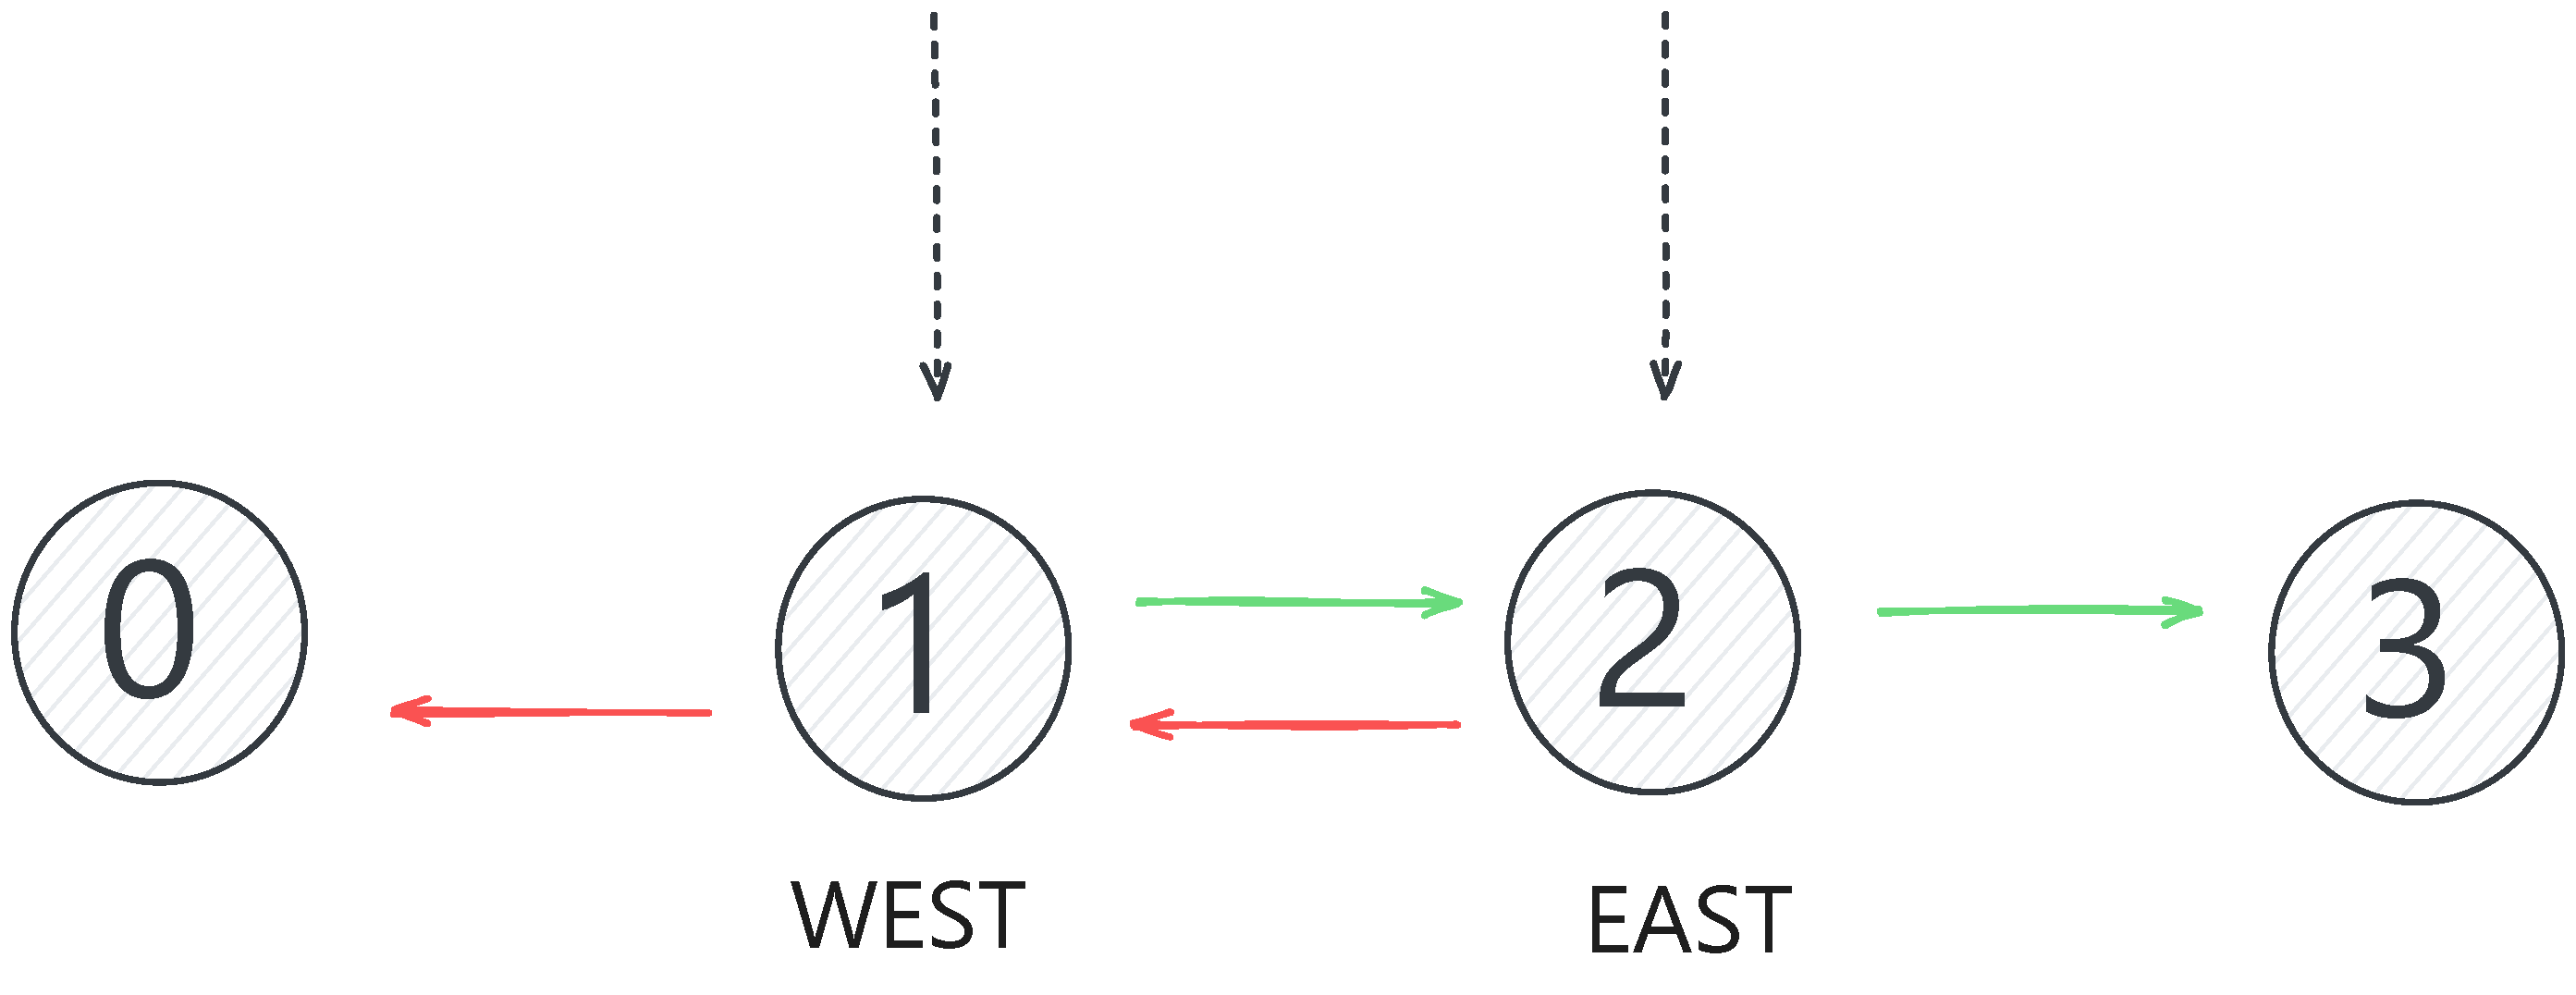
\includegraphics[width=0.8\linewidth]{plots/east_west_routing.pdf}
	\caption{Routing policy in example 5.}
	\label{fig:BgpRoutingPolicies}
\end{figure}

This SDN-controlled routing policy is realized in the pseudo code of Listing~\ref{lst:BgpNonSerializable}. T
%
The program includes a single global variable $G$, indicating if the current routing policy is the  \textcolor{ForestGreen}{green} policy ($G=1$) or the \textcolor{red}{red} policy ($G=0$).
%
The program has three types of requests:
\begin{itemize}
	
	\item 
	\textit{policy update}: represents a controller updates, and nondeterministically decides whether to update the policy (i.e., flip the value of  variable $G$) or not.
	
	\item 
	\textit{route\_from\_west}: this request represents a packet entering the network from the \textit{WEST} node (node 1).
	
	\item 
	\textit{route\_from\_east}: this request represents a packet entering the network from the \textit{EAST} node (node 2).
	
\end{itemize}


Each of the routing requests represents a single packet entering the network. The request includes a local \textit{current} variable representing the index of the current node visited. This variable is initialized as the ingress node value, and updated to emulate the routing path. There is also a \textit{visited\_east} variable (or a \textit{visited\_west} variable, depending on the request in question).
%
The return value of the \textit{route\_from\_west} requests is the sum \textit{(current+current+visited\_east)}. This is an identifier encoding all possible \textit{(current\_switch, visited\_east)} pairs.
%
The program is not serializable, as an interleaving can bring to final return value of \textit{(current+current+visited\_east)=1} (with \textit{current=0} and \textit{visited\_east=1}). This represents a routing cycle in the network, which is possible only when updated the routing policy after a a request has already been routed based on the previous policy.
Acyclic routes of this request have either a return value of 0 (in the case of [\textit{current=0}, \textit{visited\_east=0}]) or 7 (in the case of [\textit{current=3}, \textit{visited\_east=1}]).
Similarly, routing cycles are attained via non serializable executions also for the  \textit{route\_from\_east} requests.



\begin{minipage}[t]{1.0\textwidth}
	\begin{lstlisting}[caption={BGP (non serializable --- cycles can appear)},label={lst:BgpNonSerializable}]
	    // initialize accounts
	    G := 0
	    
	    request policy_update:
	    if (?):
	        G := 1  // green policy 
	    else:
	        G := 0 // red policy
			
	    request route_from_west:
	        visited_east := 0
	        current := 1
	        while (current == 2) or (current == 3): // still routing        
	            if (current == 1): // west (switch 1)
	                if (G == 1): // green policy
	                    current := 2
	                else: // red policy
	                    current := 1
	            if (current == 2): // east (switch 2)
	                visited_east := 1
	                if (G == 1): // green policy
	                    current := 3
	                else: // red policy
	                    current := 1
	 
	            yield
			
	        return current + current + visited_east
	        
	    request route_from_east:
	        ... // dual case     		        
		\end{lstlisting}
\end{minipage}






\subsection{Example 6}

\guy{suddenly I'm not so sure about this example. It is indeed sound but maybe a bit silly?}

\begin{minipage}[t]{1.0\textwidth}
	\begin{lstlisting}[caption={Snapshot-based monitor deactivation (not serializable, as it can return a sume of 0 active monitors)}]
			// initialize both monitors to be active
			N_1_ACTIVE := 1
			N_2_ACTIVE := 1
			
			request main:
				// take snapshot
				n_1_active_snapshot := N_1_ACTIVE
				n_2_active_snapshot := N_2_ACTIVE
				yield
				
				if (n_1_active_snapshot == 1) and (n_2_active_snapshot == 1):
				// if both nodes active --- choose which one to deactivate 
					if (?): 
						  N_1_ACTIVE := 0
					else:
						  N_2_ACTIVE := 0
					
				return N_1_ACTIVE + N_2_ACTIVE  // total active nodes
				
			
			request activate_n1:
				    N_1_ACTIVE := 1
			
			request activate_n2:
				    N_2_ACTIVE := 1
			
			
		\end{lstlisting}
\end{minipage}

%only 0 in non-serializable runs!

%\todo{start}

%/snapshot_isolation_directly_as_NS_with_yields

\begin{figure}[h]
	\centering
	\includegraphics[width=1.0\linewidth]{plots/snapshot\_isolation\_JSON\_with\_yields.pdf}
	\caption{Snapshot Isolation with Yields.}
	\label{fig:snapshotIsolationJsonWithYields}
\end{figure}



%/snapshot_isolation_directly_as_NS_without_yields

\begin{figure}[h]
	\centering
	\includegraphics[width=1.0\linewidth]{plots/snapshot\_isolation\_JSON\_without\_yields.pdf}
	\caption{Snapshot Isolation without Yields.}
	\label{fig:snapshotIsolationJsonWithoutYields}
\end{figure}


\todo{maybe we have: (1) a copy of the global automaton; (2) a copy of the local automaton (with yields) with coloring of edges that don't exist in the one without yields}


%\begin{figure}[h]
%	\centering
%	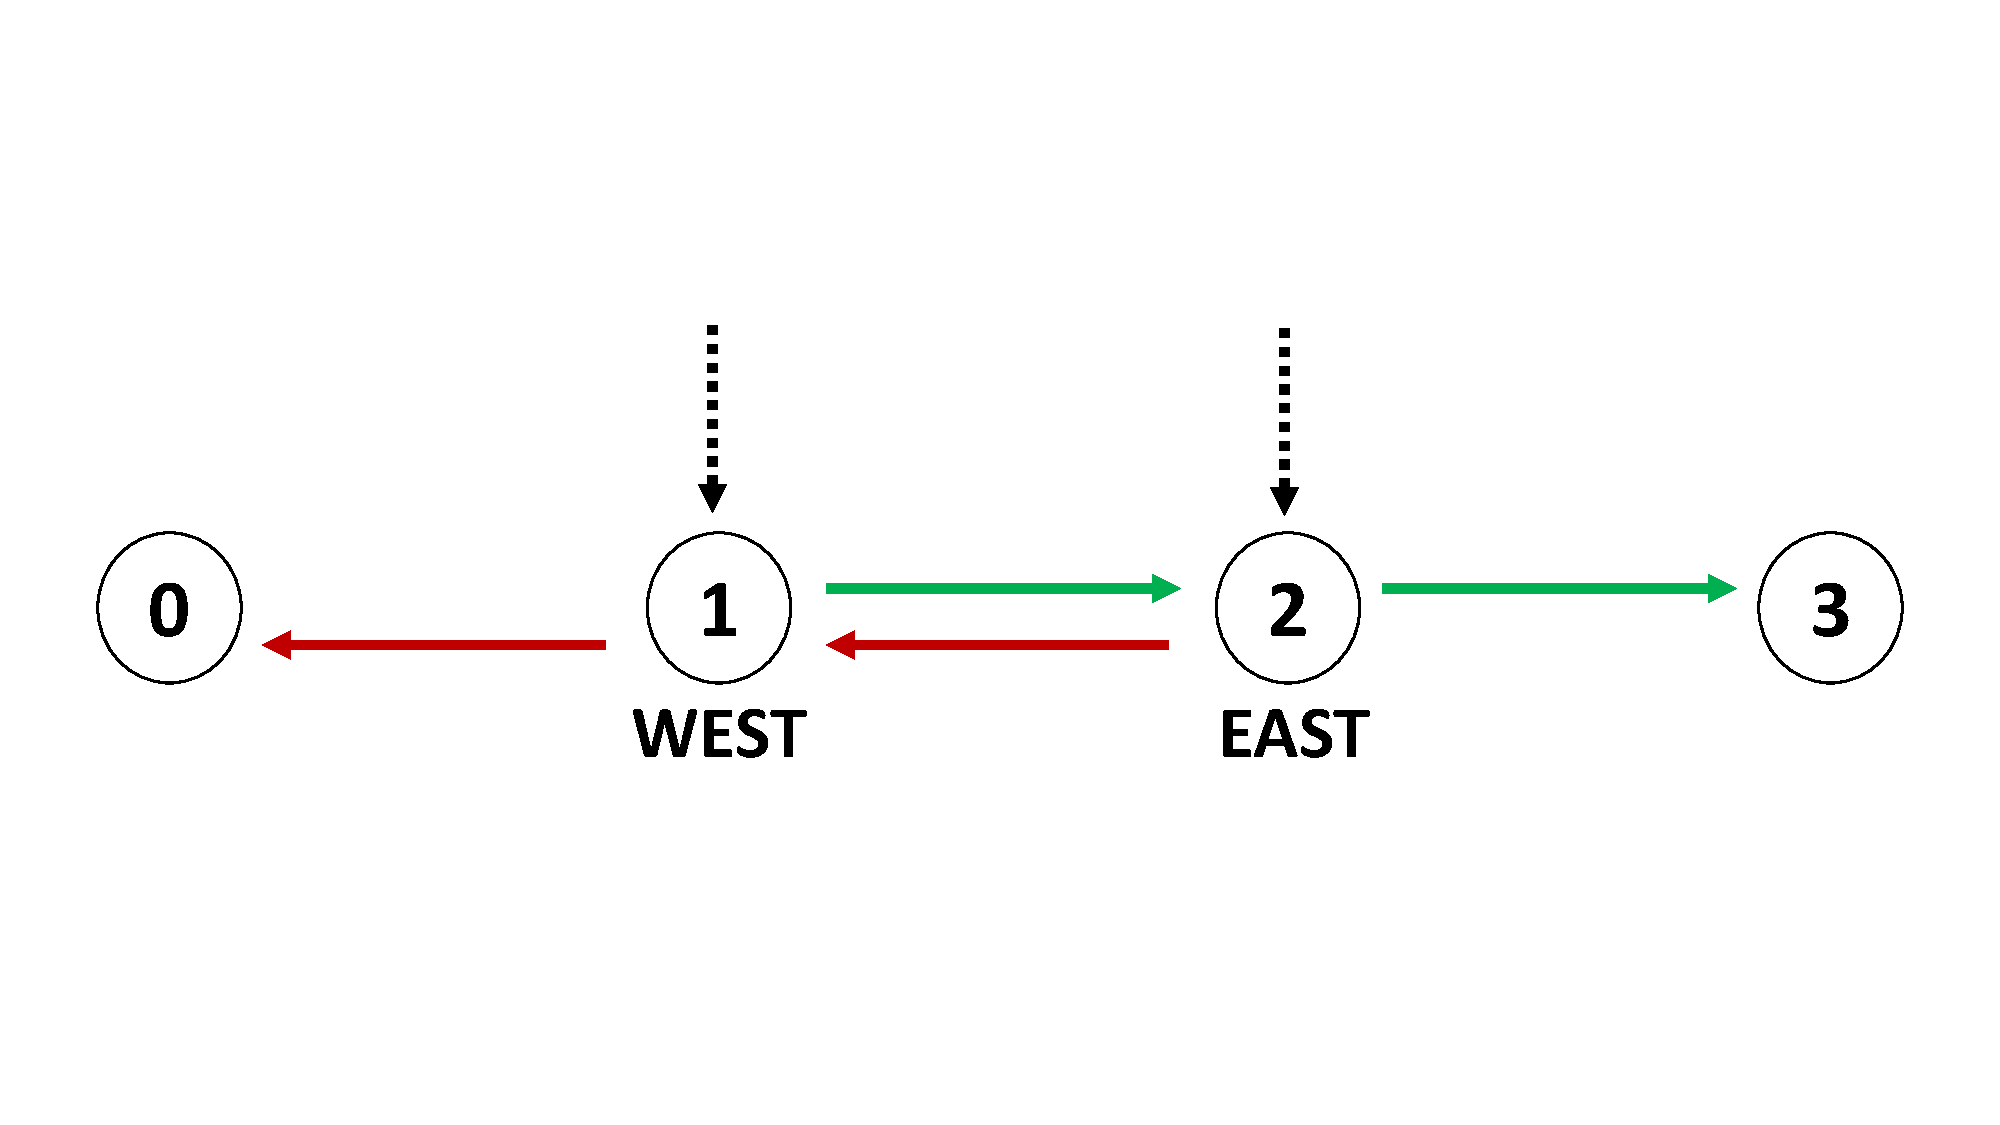
\includegraphics[width=0.65\linewidth]{plots/BgpColoredRouting.pdf}
%	\caption{Routing policy in example 7.}
%	\label{fig:pdfimage}
%\end{figure}

%\newpage
%
%
%example – 8
%
%\noindent
%\begin{minipage}[t]{0.45\textwidth}
%	\begin{lstlisting}[caption={foo (serializable)}]
%	request foo: 
%	    if (?):
%	        X := (X + 2) % 3 
%	        // no yield
%	        return X
%	
%	    else:
%	        X := (X + 1) % 3
%	        // no yield
%	        return X
%		\end{lstlisting}
%\end{minipage}
%\hfill
%\begin{minipage}[t]{0.45\textwidth}
%\begin{lstlisting}[caption={foo (non serializable)}]
%request foo: 
%     if (?):
%         X := (X + 2) % 3 
%         yield
%         return X
%
%     else:
%         X := (X + 1) % 3
%         yield
%         return X
%	\end{lstlisting}
%\end{minipage}
%
%One output that is attainable only via non-serializable executions is 
%\[
%\{(foo,1),(foo,1),(foo,1),(foo,3)\}
%\]
%
%
%%\newpage
%
%
%example – 9
%
%\noindent
%\begin{minipage}[t]{0.45\textwidth}
%	\begin{lstlisting}[caption={foo (serializable)}]
%request foo:
%    if(STOP == 0):
%        X := (X + 1) % 4
%
%    yield
%
%    if(STOP == 0):
%        X := (X + 1) % 4
%
%        STOP := ?
%        
%        if(STOP == 1):
%	        return X
%        return 0
%	\end{lstlisting}
%\end{minipage}
%\hfill
%\begin{minipage}[t]{0.45\textwidth}
%	\begin{lstlisting}[caption={foo (non serializable)}]
%request foo:
%    if(STOP == 0):
%        X := (X + 1) % 4
%
%    yield
%
%    if(STOP == 0):
%        X := (X + 2) % 4
%
%        STOP := ?
%        
%        if(STOP == 1):
%	        return X
%        return 0
%	\end{lstlisting}
%\end{minipage}



%\newpage

\section{Problem Definition}
\label{sec:problem-definition}
%\guy{Can someone check Sections 3-4-5? Especially the formulations}

Our network system (NS) syntax is defined as follows: 
%of Fig.~\ref{fig:syntax}.

\[
\begin{aligned}
	\mathbf{Expression}\quad e ::={}&{} \\
	&0 \mid 1 \mid 2 \mid \dots 
	&&\grammartag{Numeric constants}\\
	&\nondet
	&&\grammartag{Nondeterministic value: 0 or 1}\\
	&x := e
	&&\grammartag{Write to local variable}\\
	&x
	&&\grammartag{Read from local variable}\\
	&X := e
	&&\grammartag{Write to global variable}\\
	&X
	&&\grammartag{Read from global variable}\\
	&e_1 == e_2
	&&\grammartag{Equality test}\\
	&e_1 ; e_2
	&&\grammartag{Sequencing}\\
	&\ifkw(e_1)\{e_2\}\elsekw\{e_3\}
	&&\grammartag{Conditional}\\
	&\whilekw(e_1)\{e_2\}
	&&\grammartag{While loop}\\
	&\yieldkw
	&&\grammartag{Yields to scheduler}\\[1em]
	\mathbf{Program}\quad p ::={}&{} \\
	&\requestkw\ name_1\{e_1\}
	&&\grammartag{Set of request handlers}\\
	&\quad\vdots\\
	&\requestkw\ name_n\{e_n\}
\end{aligned}
\]

%
%
%\begin{figure}[!htbp]
%    \begin{align*}
%    \mathbf{Expression}\quad e ::= &&& \\
%       | & \quad 0 \mid 1 \mid 2 \mid \ldots                                && \grammartag{Numeric constants} \\
%       | & \quad \nondet                                 && \grammartag{Nondeterministic value: 0 or 1}\\
%       | & \quad x := e                            && \grammartag{Write to local variable field} \\
%       | & \quad x                                 && \grammartag{Read from local variable field} \\
%       | & \quad X := e                            && \grammartag{Write to global  variable} \\
%       | & \quad X                                 && \grammartag{Read from global  variable} \\
%       | & \quad e_1 == e_2                        && \grammartag{Equality test} \\
%       | & \quad e_1 ; e_2                         && \grammartag{Sequencing} \\
%       | & \quad \ifkw(e_1)\{\ e_2\ \}\elsekw\{\ e_3\ \} && \grammartag{Conditional} \\
%       | & \quad \whilekw(e_1)\{\ e_2\ \}              && \grammartag{While loop} \\
%       | & \quad \yieldkw                      && \grammartag{Yields to scheduler}\\[1em]
%    \mathbf{Program}\quad p ::=
%        & \quad \requestkw\ name_1\ \{\ e_1\ \}&&\grammartag{Set of request handlers}\\[-0.5em]
%        & \quad \qquad \vdots &&\\
%        & \quad \requestkw\ name_n\ \{\ e_n\ \}\ 
%    \end{align*}
%    \caption{Syntax of expressians and programs}
%    \label{fig:syntax}
%\end{figure}
    %
This NS setting is motivated by software-defined networking systems. In the networking domain, spawning a request corresponds to sending a packet, with each local variable mapped to a unique packet header field; global variables correspond to variables on programmable switches, as they are shared among all requests visiting the switch. Throughout this paper, we use the term \emph{request} to refer to a concurrent computation unit. 
    
   
A network system $\mathcal{N}$ is a tuple $(G, L, \mathit{REQ}, \mathit{RESP}, g_0, \delta, \mathit{req}, \mathit{resp})$ where:
\begin{itemize}
\item $G$ is a set of global states (assignments to all global variables)
\item $L$ is a set of local states (local variable values and remaining program to execute)
\item $\mathit{REQ}$ is a set of request types (marked {\color{ForestGreen}$\blacklozenge_\text{req}$})
\item $\mathit{RESP}$ is a set of response types (marked {\color{red}$\blacklozenge_\text{resp}$})
\item $g_0 \in G$ is the initial global state
\item $\mathit{req} \subseteq \mathit{REQ} \times L$ maps each request type to its initial local state
\item $\mathit{resp} \subseteq L \times \mathit{RESP}$ maps final local states to response types
\item $\delta \subseteq (G \times L) \times (G \times L)$ defines atomic execution steps that update both global and local state
\end{itemize}

\begin{definition}[Request and Response]
A \emph{request} $r \in \mathit{REQ}$ represents the initiation of a concurrent computation unit. Each request has an associated handler expression from the program syntax that defines its behavior.
A \emph{response} $s \in \mathit{RESP}$ represents the value returned by a request after its execution terminates.
The pair $(r, s) \in \mathit{REQ} \times \mathit{RESP}$ captures the complete input-output behavior of a single request execution.
\end{definition}




\begin{figure}[t]
    \centering
    \renewcommand{\arraystretch}{1.6}
    \[
    \begin{array}{c}
    \textbf{States and Transitions:}
    \\
    \quad
    \text{A (global) \emph{network state} is a triple }(g,\mathcal{P},M)\text{ where:}
    \\
    \quad
    g \in G \text{ is the current global state,}
    \\
    \quad
    \mathcal{P} \in \text{Multiset}(L \times \mathit{REQ}) \text{ is a multiset of in-flight requests (threads),}
    \\
    \quad
    M \in \text{Multiset}(\mathit{REQ} \times \mathit{RESP}) \text{ is a multiset of request/response pairs already completed.}
    \end{array}
    \]

    \[
    \begin{array}{c}
    \textbf{Initial state:}
    \\
    \quad (g_0,\,\varnothing,\,\varnothing)
    \end{array}
    \]

    \[
    \begin{array}{c}
    \textbf{Transition rules:}
    \\[1em]
    \text{(New Request)}\quad\infer{
    ({\color{ForestGreen}\blacklozenge_\text{r}},\ell)\,\in\,\mathit{req}
    }
    {(g,\;\mathcal{P},\;M) \;\longrightarrow\; (g,\;\mathcal{P} \uplus \{(\ell,{\color{ForestGreen}\blacklozenge_\text{r}})\},\;M)}
    \\[2em]
    \text{(Processing Step)}\quad\infer{
    ((g,\ell),\,(g',\ell')) \,\in\, \delta
    }
    {(g,\;\mathcal{P} \uplus \{(\ell,{\color{ForestGreen}\blacklozenge_\text{r}})\},\;M) \;\longrightarrow\; (g',\;\mathcal{P} \uplus \{(\ell',{\color{ForestGreen}\blacklozenge_\text{r}})\},\;M)}
    \\[2em]
    \text{(Response)}\quad\infer{
    (\ell,{\color{red}\blacklozenge_\text{s}})\,\in\,\mathit{resp}
    }
    {(g,\;\mathcal{P} \uplus \{(\ell,{\color{ForestGreen}\blacklozenge_\text{r}})\},\;M) \;\longrightarrow\; (g,\;\mathcal{P},\;M \uplus \{({\color{ForestGreen}\blacklozenge_\text{r}},{\color{red}\blacklozenge_\text{s}})\})}
    \end{array}
    \]

    \[
    \begin{array}{c}
    \textbf{Complete runs:}
    \\
    \quad (g_0,\,\varnothing,\,\varnothing) \;\longrightarrow\; (g_1,\,\mathcal{P}_1,\,M_1) \;\longrightarrow\; \cdots \;\longrightarrow\; (g_n,\,\mathcal{P}_{n-1},\,M_{n-1}) \;\longrightarrow\; (g_n,\,\varnothing,\,M_n)
    \\[1em]
    \textbf{Interleaved run: } \text{the } \mathcal{P}_i \text{ can have more than one request, and } \mathcal{P}_n = \varnothing \\
    \textbf{Serial run: } \text{ each } \mathcal{P}_i \text{ has at most one request, and } \mathcal{P}_n = \varnothing\\
    \text{Int}(\mathcal{N}) = \{ M \in \text{Multiset}(\mathit{REQ} \times \mathit{RESP}) \mid \exists \text{ interleaved run } (g_0,\,\varnothing,\,\varnothing) \;\longrightarrow^*\; (g_n,\,\varnothing,\,M) \}\\
    \text{Ser}(\mathcal{N}) = \{ M \in \text{Multiset}(\mathit{REQ} \times \mathit{RESP}) \mid \exists \text{ serial run } (g_0,\,\varnothing,\,\varnothing) \;\longrightarrow^*\; (g_n,\,\varnothing,\,M) \}\\
    \end{array}
    \]

    \caption{State-transition rules for executions of
    \(\mathcal{N} = (G, L, \mathit{REQ}, \mathit{RESP}, g_0, \delta, \mathit{req}, \mathit{resp})\).
    A transition \(\longrightarrow\) modifies the triple \((g,\mathcal{P}, M)\) by either (1) introducing a new request, (2) processing a request step via \(\delta\), or (3) consuming a request to produce its response.  When no more steps are possible, the result set \(M\) is the final multiset of request/response pairs that arose during the run.
    Runs are called \emph{serial} if there is at most one request in flight at any time, whereas \emph{interleaved} runs may have multiple requests in flight at once.}
    \label{fig:network-transitions}
\end{figure}

\begin{definition}[Serializability]
A network system $\mathcal{N}$ is \emph{serializable} if $\text{Int}(\mathcal{N}) = \text{Ser}(\mathcal{N})$, meaning every multiset of request/response pairs achievable through interleaved execution can also be achieved through some serial execution.
\end{definition}

%\guy{Nicolas/Jules can you take a look at the other definition that I masked in the latex below? Is the current one good enough?}

%\begin{definition}[Interleaved executions \(\mathrm{Int}(\mathcal{N})\)]
%    Let \(\mathcal{N} = (G, L, \mathit{Req}, \mathit{Res}, g_0, \delta, \mathit{req}, \mathit{resp})\).
%    An \emph{interleaved execution} begins in global state \(g = g_0\) with no packets in flight.
%    At any point, one may:
%    \begin{itemize}
%        \item introduce a new request \(r \in \mathit{Req}\), producing an in-flight packet \(\ell \in L\) if \((r,\ell) \in \mathit{req}\);
%        \item take an in-flight packet \(\ell\) and transition \(\ell \mapsto \ell'\) and \(g \mapsto g'\) if \(((g,\ell),(g',\ell'))\in\delta\);
%        \item consume an in-flight packet \(\ell\) to produce a response \(s\) if \((\ell,s)\in \mathit{resp}\).
%    \end{itemize}
%    Each request \(r\) must eventually yield exactly one corresponding response \(s\) in a valid execution.
%    The set of all finite multisets of \((r,s)\) pairs realizable by such interleavings is:
%    \[
%        \mathrm{Int}(\mathcal{N})
%        \;=\;
%        \bigl\{
%        M \;\in\; \text{Multiset}(\mathit{Req}\times \mathit{Res})
%        \;\mid\;
%        M \text{ is realized by some interleaved run of }\mathcal{N}
%        \bigr\}.
%    \]
%\end{definition}
%
%\begin{definition}[Serial executions \(\mathrm{Ser}(\mathcal{N})\)]
%In a \emph{serial} execution, requests are processed one at a time:
%\begin{enumerate}
%    \item Start in \(\,g_0\).
%    \item Take a single request \(r\in \mathit{Req}\), convert it to a packet, process that packet until a response \(s\in \mathit{Res}\) is produced.
%    \item Update the global state accordingly and repeat with the next request.
%\end{enumerate}
%No two requests overlap in processing.
%The set of all finite multisets of \((r,s)\) pairs realizable by such one-at-a-time runs is:
%\[
%    \mathrm{Ser}(\mathcal{N})
%    \;=\;
%    \bigl\{
%    M \;\in\; \text{Multiset}(\mathit{Req}\times \mathit{Res})
%    \;\mid\;
%    M \text{ is realized by some serial run of }\mathcal{N}
%    \bigr\}.
%\]
%\end{definition}



%\begin{theorem}[Serial Equivalence]
%\label{thm:ser-eq-ser}
%Whether
%\(
%    \mathrm{Ser}(\mathcal{N}) \;=\; \mathrm{Ser}(\mathcal{N})
%\)
%holds is decidable.
%\end{theorem}
%
%\begin{theorem}[Interleaved Equivalence]
%\label{thm:int-eq-int}
%Whether
%\(
%    \mathrm{Int}(\mathcal{N}) \;=\; \mathrm{Int}(\mathcal{N})
%\)
%holds is undecidable.
%\end{theorem}

\subsection{NS Example: Non-Serializability }
\label{sec:ns-non-serializable}

Recall the code snippet from the simple, non-serializable example presented in Listing~\ref{lst:MotivatingExample2NonSer}. We can represent its NS with the following mapping:

\begin{itemize}
\item 
The set $G$ is defined as $G=\{[X=0], [X=1]\}$

\item 
The initial global $g_0$ state is defined as $g_0 = [X=0]$.

\item 
We define $L$ as all pairs of local states (assignments such as $[y=0], [y=1]$) and ``remaining'' programs.

\item 
The set of requests is $REQ = \{{\color{ForestGreen}\blacklozenge_\text{main}}\}$

\item 
The set of responses is $RESP = \{{\color{red}\blacklozenge_0},{\color{red}\blacklozenge_1}\}$

\end{itemize}

We define the three mappings $req$, $resp$, and $\delta$ as follows:
%\begin{minipage}[t]{0.3\textwidth}
%	\begin{lstlisting}[caption={Without yield or lock (serializable)}]
%	request main: 
%			X := 1 
%			yield
%			y := X 
%			X := 0
%			return y 
%		\end{lstlisting}
%\end{minipage}


\[
req \coloneq 
\Bigg\{
\Bigg[
\begin{array}{c c c}
	% ---- the 'main' diamond unchanged
	\begin{tikzpicture}[baseline=(textnode.base)]
		\node[
		draw=black,
		fill=ForestGreen!20,
		text=black,
		diamond,
		aspect=2,
		inner sep=4pt
		] (textnode) {main};
	\end{tikzpicture}
	&
	\!\!\rightarrow\!\! 
	&
	\bigg(
	\begin{tabular}{c c}
		% ---- now a brighter yellow, dashed border
		\begin{tikzpicture}[baseline=(ybox.base)]
			\node[
			draw=black,           % black border
			%dashed,               % dashed border style
			line width=0.8pt,     % dash thickness
			%dash pattern=on 3pt off 2pt, % custom dash pattern
			fill=brightyellow,    % extra-bright yellow fill
			text=black,           % black text
			rectangle,            % shape
			rounded corners=1pt,  % slight rounding
			inner sep=2pt         % padding
			] (ybox) {\large y=0};
		\end{tikzpicture}
		,\quad
		&
		\begin{minipage}{0.14\linewidth}
			\begin{lstlisting}[language=CustomPseudoCode,numbers=none]
X := 1 
yield 
y := X + 1
X := 0
return y
			\end{lstlisting}
		\end{minipage}
	\end{tabular}
	\bigg)
\end{array}
\Bigg]
\Bigg\}
\]





\[
resp \coloneq
\Bigg \{
\Bigg [ 
\begin{array}{c c c}
\bigg(
\begin{tabular}{c c}
		\begin{tikzpicture}[baseline=(ybox.base)]
	\node[
	draw=black,           % black border
	%dashed,               % dashed border style
	line width=0.8pt,     % dash thickness
	%dash pattern=on 3pt off 2pt, % custom dash pattern
	fill=brightyellow,    % extra-bright yellow fill
	text=black,           % black text
	rectangle,            % shape
	rounded corners=1pt,  % slight rounding
	inner sep=2pt         % padding
	] (ybox) {\large y=0};
\end{tikzpicture} ,\quad & 
\begin{minipage}{0.11\linewidth}
		\begin{lstlisting}[language=CustomPseudoCode,numbers=none]
// end
			\end{lstlisting}
	\end{minipage}
\end{tabular}
\bigg)
&
\rightarrow
&
\text{
\begin{tikzpicture}[baseline=(textnode.base)]
		\node[
		draw=black,                      % ← outline color
		fill=RedViolet!20,            % ← light green fill
		text=black,
		diamond,
		aspect=2,
		inner sep=4pt
		] (textnode) {0};
	\end{tikzpicture}
} 
\end{array}
\Bigg ]
,
%\quad
\Bigg [ 
\begin{array}{c c c}
\bigg(
\begin{tabular}{c c}
		\begin{tikzpicture}[baseline=(ybox.base)]
	\node[
	draw=black,           % black border
	%dashed,               % dashed border style
	line width=0.8pt,     % dash thickness
	%dash pattern=on 3pt off 2pt, % custom dash pattern
	fill=brightyellow,    % extra-bright yellow fill
	text=black,           % black text
	rectangle,            % shape
	rounded corners=1pt,  % slight rounding
	inner sep=2pt         % padding
	] (ybox) {\large y=1};
\end{tikzpicture} ,\quad & 
\begin{minipage}{0.11\linewidth}
		\begin{lstlisting}[language=CustomPseudoCode,numbers=none]
// end
			\end{lstlisting}
	\end{minipage}
\end{tabular}
\bigg)
&
\rightarrow
&
\text{
\begin{tikzpicture}[baseline=(textnode.base), scale=0.7]
		\node[
		draw=black,                      % ← outline color
		fill=RedViolet!20,            % ← light green fill
		text=black,
		diamond,
		aspect=2,
		inner sep=4pt
		] (textnode) {1};
	\end{tikzpicture}
} 
\end{array}
\Bigg ] 
\Bigg \} 
\]





\[
\begin{array}{l}
\delta := 
\Bigg\{ 
\Bigg[
\Bigg(
\begin{tikzpicture}[baseline=(ybox.base)]
	\node[
	draw=black,           % black border
	%dashed,               % dashed border style
	line width=0.8pt,     % dash thickness
	%dash pattern=on 3pt off 2pt, % custom dash pattern
	fill=lightchacki,    % extra-bright yellow fill
	text=black,           % black text
	rectangle,            % shape
	rounded corners=1pt,  % slight rounding
	inner sep=2pt         % padding
	] (ybox) {\large X=0};
\end{tikzpicture} ,\quad
\bigg(
\begin{tabular}{c c}
		\begin{tikzpicture}[baseline=(ybox.base)]
	\node[
	draw=black,           % black border
	%dashed,               % dashed border style
	line width=0.8pt,     % dash thickness
	%dash pattern=on 3pt off 2pt, % custom dash pattern
	fill=brightyellow,    % extra-bright yellow fill
	text=black,           % black text
	rectangle,            % shape
	rounded corners=1pt,  % slight rounding
	inner sep=2pt         % padding
	] (ybox) {\large y=0};
\end{tikzpicture} ,\quad & 
\begin{minipage}{0.14\linewidth}
		\begin{lstlisting}[language=CustomPseudoCode,numbers=none]
X := 1
yield
y := X + 1
X := 0
return y
			\end{lstlisting}
	\end{minipage}
\end{tabular}
\bigg)
\Bigg)
\rightarrow
\Bigg(
\begin{tikzpicture}[baseline=(ybox.base)]
	\node[
	draw=black,           % black border
	%dashed,               % dashed border style
	line width=0.8pt,     % dash thickness
	%dash pattern=on 3pt off 2pt, % custom dash pattern
	fill=lightchacki,    % extra-bright yellow fill
	text=black,           % black text
	rectangle,            % shape
	rounded corners=1pt,  % slight rounding
	inner sep=2pt         % padding
	] (ybox) {\large X=1};
\end{tikzpicture} ,\quad
\bigg(
\begin{tabular}{c c}
		\begin{tikzpicture}[baseline=(ybox.base)]
	\node[
	draw=black,           % black border
	%dashed,               % dashed border style
	line width=0.8pt,     % dash thickness
	%dash pattern=on 3pt off 2pt, % custom dash pattern
	fill=brightyellow,    % extra-bright yellow fill
	text=black,           % black text
	rectangle,            % shape
	rounded corners=1pt,  % slight rounding
	inner sep=2pt         % padding
	] (ybox) {\large y=0};
\end{tikzpicture} ,\quad & 
\begin{minipage}{0.14\linewidth}
		\begin{lstlisting}[language=CustomPseudoCode,numbers=none]
y := X + 1
X := 0
return y
			\end{lstlisting}
	\end{minipage}
\end{tabular}
\bigg)
\Bigg)
\Bigg]
\bigcup\ \ldots, \\[1em]
\quad
\ldots
\bigcup\ 
\Bigg[
\Bigg(
\begin{tikzpicture}[baseline=(ybox.base)]
	\node[
	draw=black,           % black border
	%dashed,               % dashed border style
	line width=0.8pt,     % dash thickness
	%dash pattern=on 3pt off 2pt, % custom dash pattern
	fill=lightchacki,    % extra-bright yellow fill
	text=black,           % black text
	rectangle,            % shape
	rounded corners=1pt,  % slight rounding
	inner sep=2pt         % padding
	] (ybox) {\large X=1};
\end{tikzpicture}  ,\quad
\bigg(
\begin{tabular}{c c}
		\begin{tikzpicture}[baseline=(ybox.base)]
	\node[
	draw=black,           % black border
	%dashed,               % dashed border style
	line width=0.8pt,     % dash thickness
	%dash pattern=on 3pt off 2pt, % custom dash pattern
	fill=brightyellow,    % extra-bright yellow fill
	text=black,           % black text
	rectangle,            % shape
	rounded corners=1pt,  % slight rounding
	inner sep=2pt         % padding
	] (ybox) {\large y=0};
\end{tikzpicture} ,\quad & 
\begin{minipage}{0.14\linewidth}
		\begin{lstlisting}[language=CustomPseudoCode,numbers=none]
y := X + 1
X := 0
return y
			\end{lstlisting}
	\end{minipage}
\end{tabular}
\bigg)
\Bigg)
\rightarrow
\Bigg(
\begin{tikzpicture}[baseline=(ybox.base)]
	\node[
	draw=black,           % black border
	%dashed,               % dashed border style
	line width=0.8pt,     % dash thickness
	%dash pattern=on 3pt off 2pt, % custom dash pattern
	fill=lightchacki,    % extra-bright yellow fill
	text=black,           % black text
	rectangle,            % shape
	rounded corners=1pt,  % slight rounding
	inner sep=2pt         % padding
	] (ybox) {\large X=0};
\end{tikzpicture} ,\quad
\bigg(
\begin{tabular}{c c}
		\begin{tikzpicture}[baseline=(ybox.base)]
	\node[
	draw=black,           % black border
	%dashed,               % dashed border style
	line width=0.8pt,     % dash thickness
	%dash pattern=on 3pt off 2pt, % custom dash pattern
	fill=brightyellow,    % extra-bright yellow fill
	text=black,           % black text
	rectangle,            % shape
	rounded corners=1pt,  % slight rounding
	inner sep=2pt         % padding
	] (ybox) {\large y=1};
\end{tikzpicture} ,\quad & 
\begin{minipage}{0.11\linewidth}
		\begin{lstlisting}[language=CustomPseudoCode,numbers=none]
// end
			\end{lstlisting}
	\end{minipage}
\end{tabular}
\bigg)
\Bigg)
\Bigg]
\bigcup\ \ldots
\Bigg\}
\end{array}
\]

%\todo{emphasize that there are states we didn't add}

We note that we depicted only part of the states that are \textit{reachable}, in our finite-state setting.
%
Next, we present in Fig.~\ref{fig:code2ExampleNS} the explicit network system that depicts the program, which serves as a mapping from requests ({\color{ForestGreen}$\blacklozenge_\text{main}$}) to responses ({\color{red}$\blacklozenge_0$}, {\color{red}$\blacklozenge_1$}).



\begin{figure}[!htbp]
	\centering
	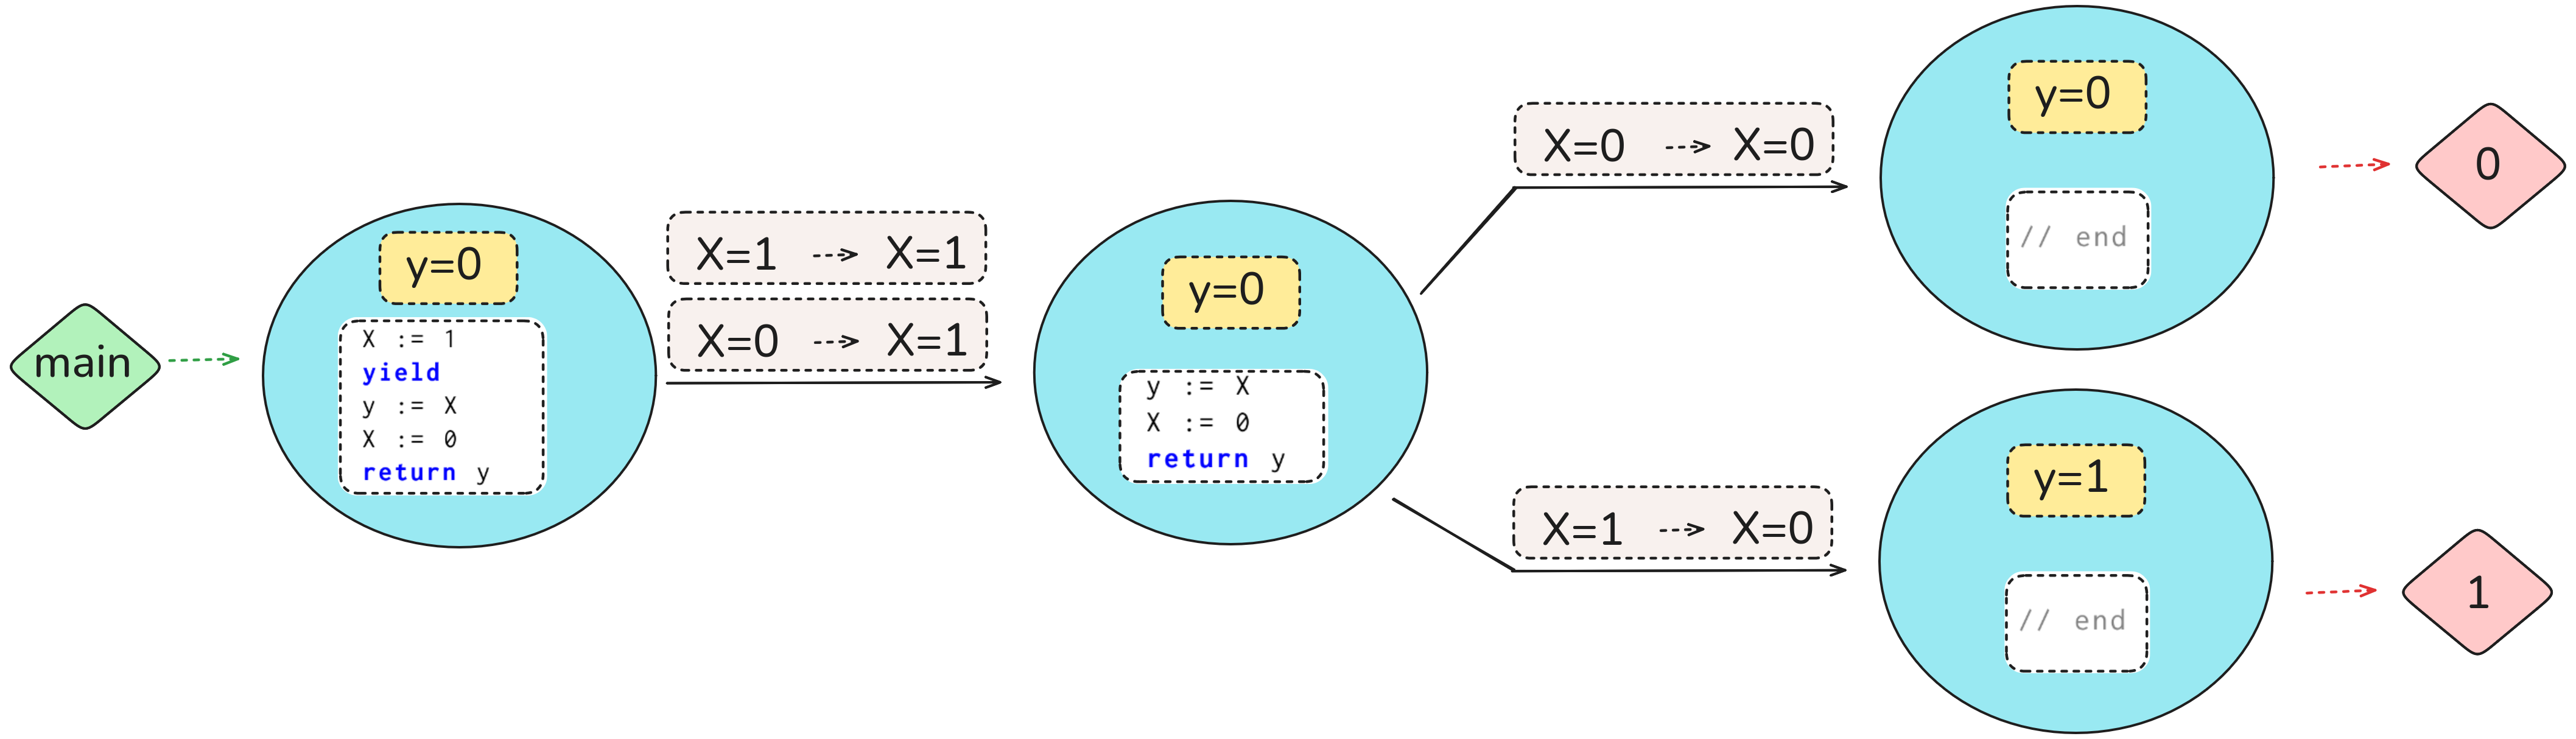
\includegraphics[width=1.1\textwidth]{plots/code_2_NS.png}
	\caption{Network system for the program in Listing~\ref{lst:MotivatingExample2NonSer}.}
	\label{fig:code2ExampleNS}
\end{figure}

%
%%
%The NS allows us to also extract the NFA encoding all serial executions. The states encode the global variable values, and the edges encode request/response pairs for all serial executions. As can be seen, serial executions can produce only pairs of the type ({\color{ForestGreen}$\blacklozenge_\text{main}$/{\color{red}$\blacklozenge_1$}}):
%
%\begin{figure}[!htbp]
%	\centering
%	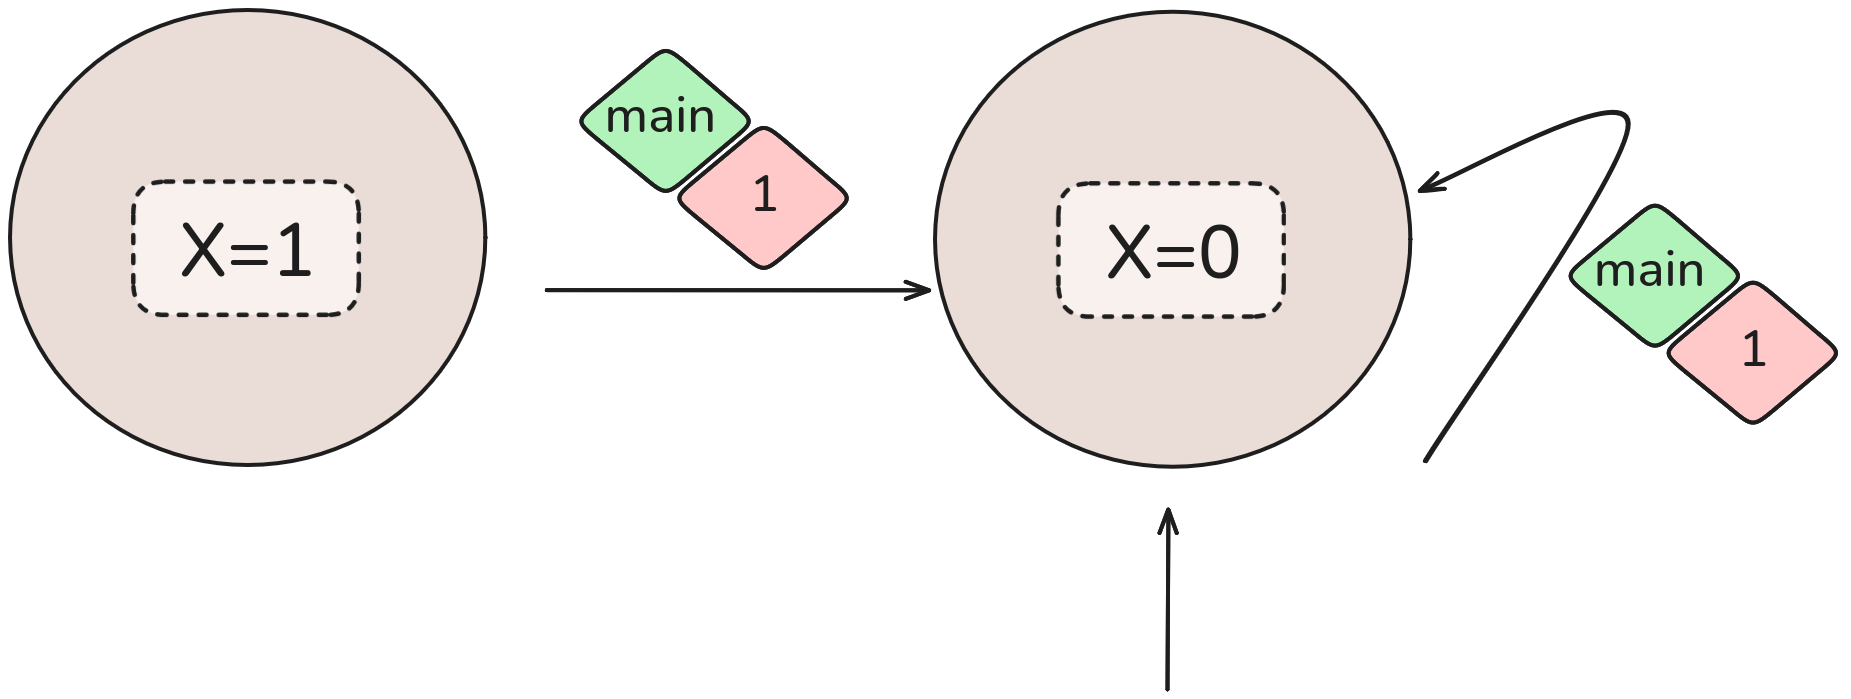
\includegraphics[width=0.5\textwidth,trim=0 0 0 0,clip]{plots/code_2_NFA.png}
%	\caption{NFA for serialized executions of Listing~\ref{lst:MotivatingExample2NonSer} program.}
%	\label{fig:code2ExampleNFA}
%\end{figure}
%
%Finally, the NS allows to generate the following Petri Net, encoding all possible interleavings of our program:
%
%\begin{figure}[!htbp]
%	\centering
%	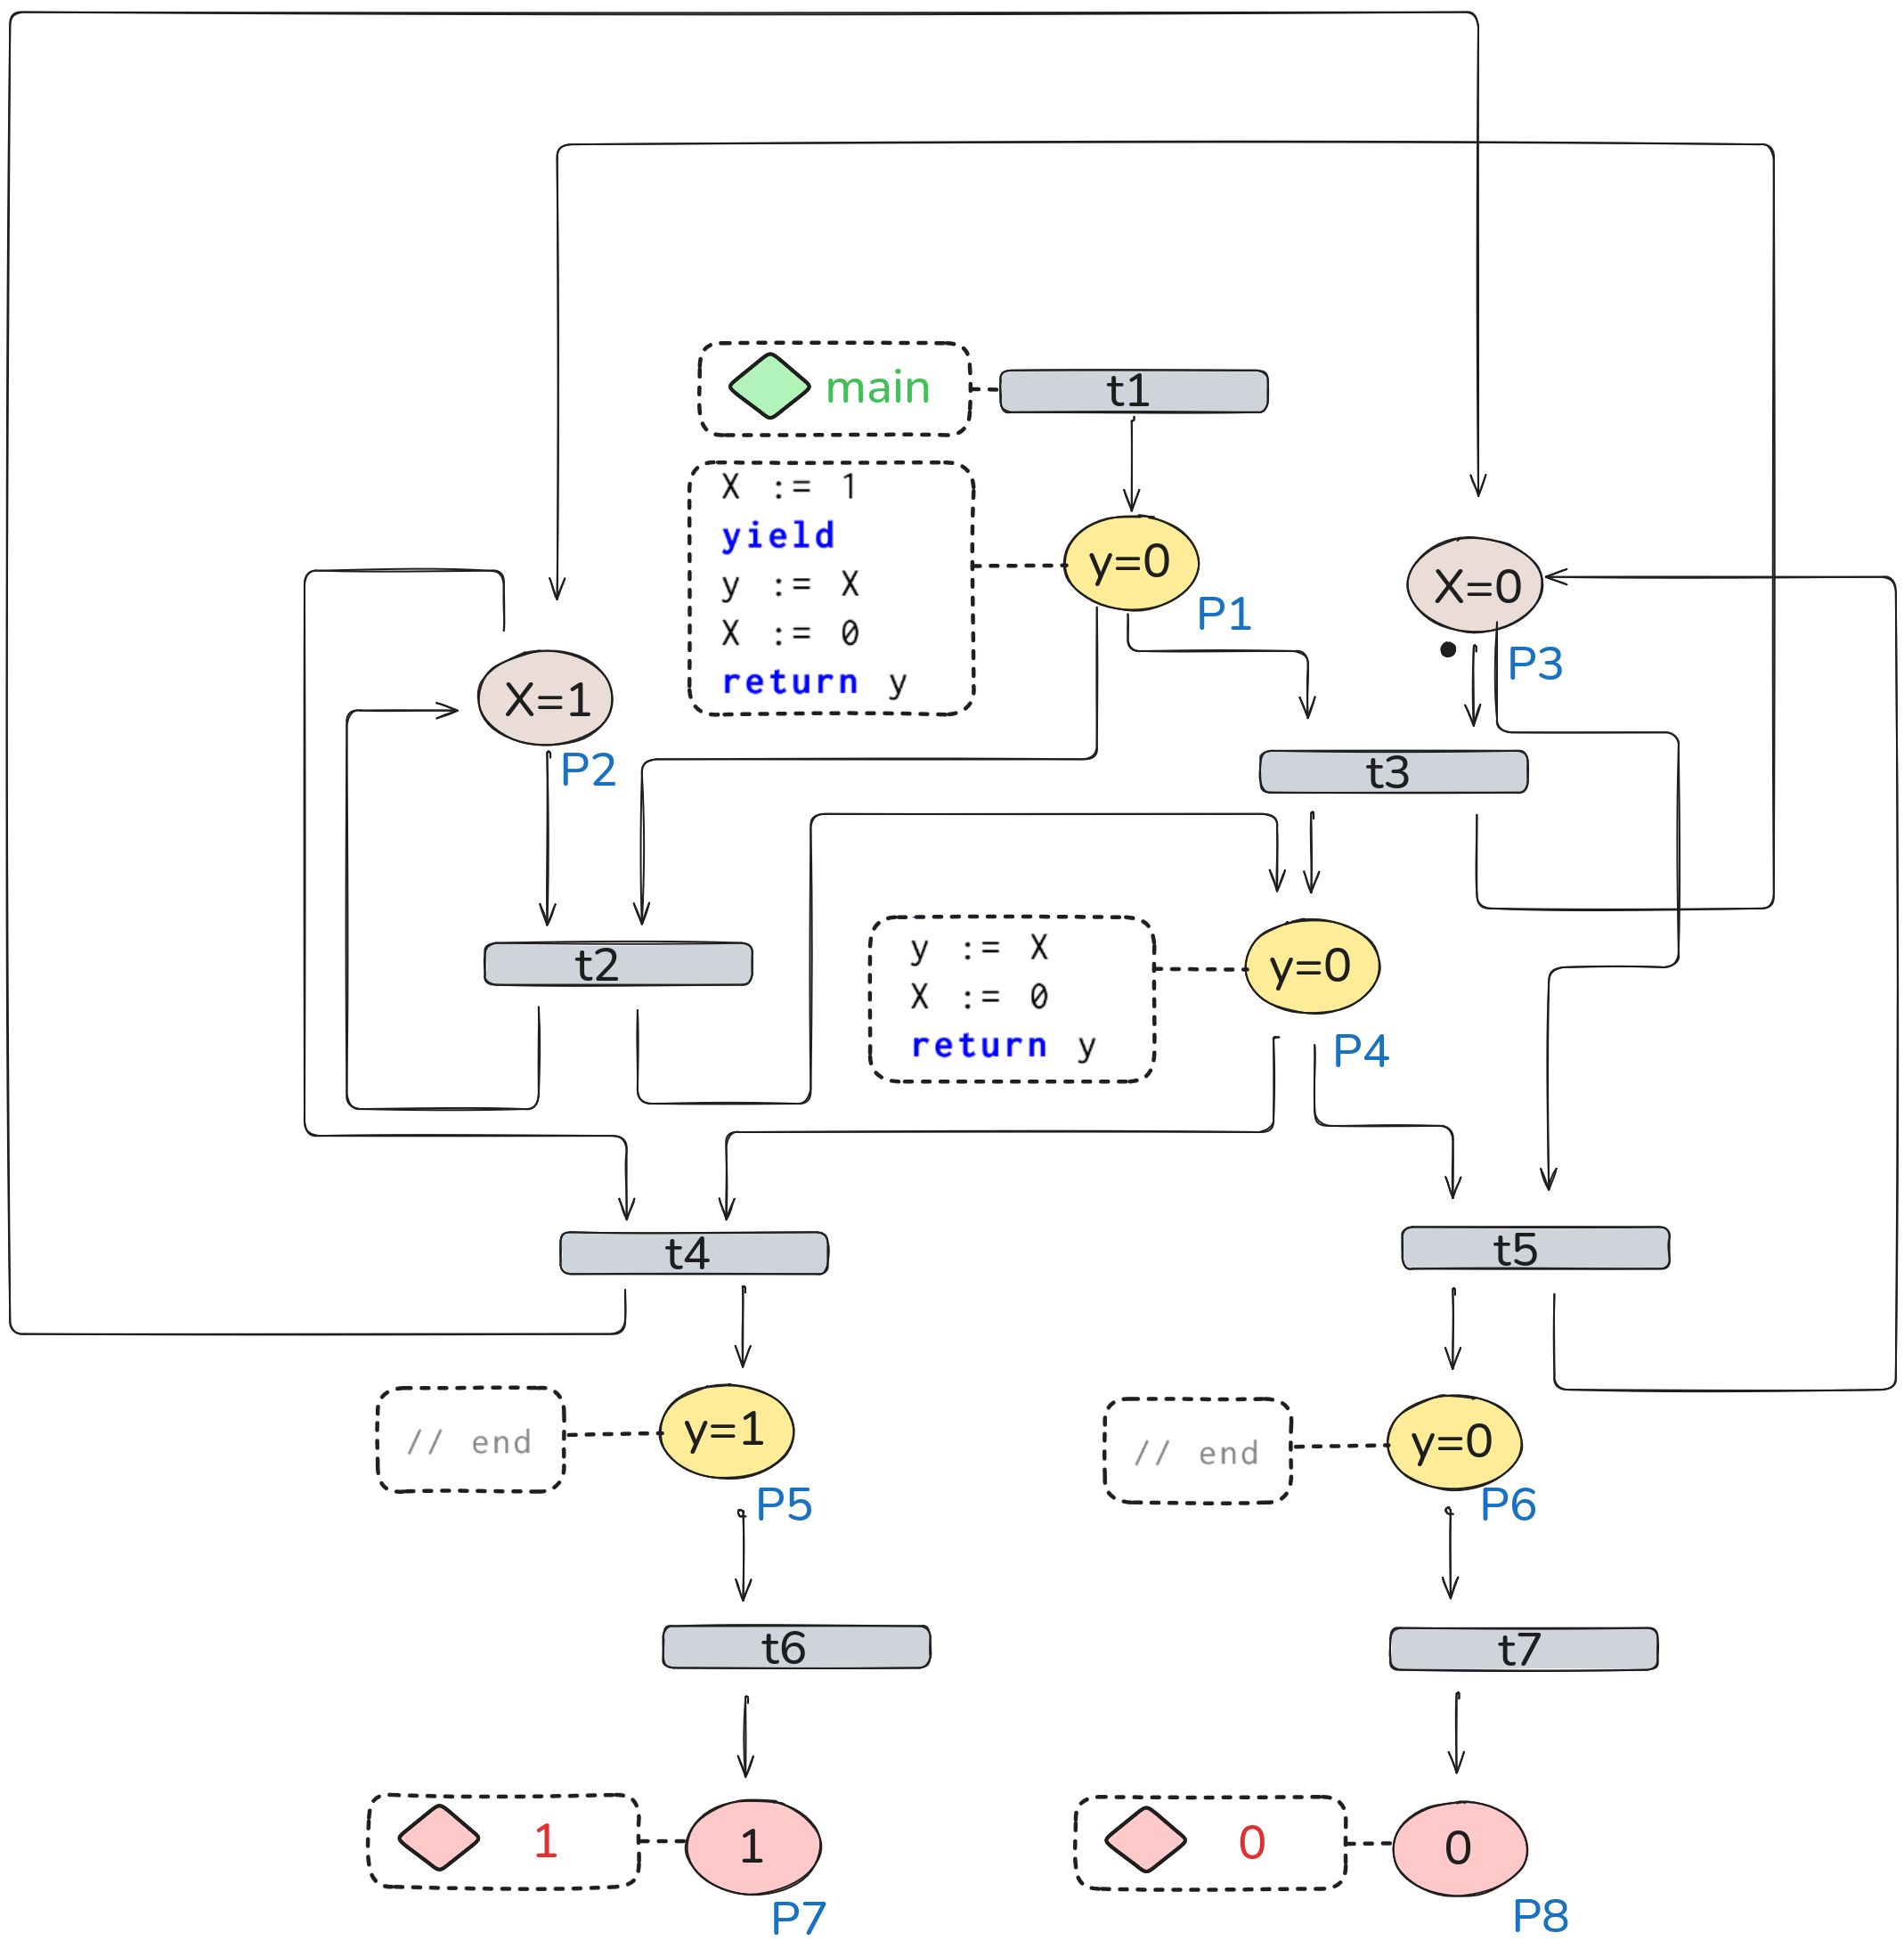
\includegraphics[width=0.7\textwidth]{plots/code_2_PN_with_annotation.png}
%	\caption{Petri Net for interleaving executions of Listing~\ref{lst:MotivatingExample2NonSer} program. Note that there is no firing sequence that can reach the place representing a response of ``0'', i.e., the bottom right place.}
%	\label{fig:code2ExamplePN}
%\end{figure}
%
%The places represent the $\delta$ transitions of our NS --- encoding either a ``step'' of our program, or spawning a request ($t_1$, which  corresponds to spawning request {\color{ForestGreen}$\blacklozenge_\text{main}$}), or returning a responds, e.g. transitions $t_6,t_7$ that corresponds to outputting responses {\color{red}$\blacklozenge_1$},{\color{red}$\blacklozenge_0$}.
%%
%Some places (\textcolor{blue}{$P_2$},\textcolor{blue}{$P_3$}) corresponds to the global state, while others ($P_1,P_4,P_5,P_6$) corresponds to the local state of an in-flight request.
%%
%Each token corresponds to a single packet, or (in the case of the global-variable-encoding places), to the global state of the program.
%
%
%
%Regarding the aforementioned program, we automatically generate the following LTL reachability query for the Petri net of Figure~\ref{fig:code1ExamplePN} (which, if satisfiable, indicates the program is not serializable):
%
%\todo{fix the "exists Marking M"}
%
%\[
%\exists\,M.\; 
%P_1 = 0 \wedge 
%\textcolor{blue}{P_2} \ge 0 \wedge \textcolor{blue}{P_3} \ge 0  \wedge P_4 = 0
%\wedge P_5 = 0 \wedge P_6 = 0 \wedge \textcolor{red}{P_7} = 0 \wedge \textcolor{red}{P_8} \ge 1.
%\]
%This asserts the existence of a marking with no tokens on $P_1,P_4,P_5,P_6$, exactly zero tokens on $\textcolor{red}{P_7}$, at least one token on $\textcolor{red}{P_8}$, and arbitrary tokens on $\textcolor{blue}{P_2},\textcolor{blue}{P_3}$.  In fact, the target marking
%\[
%M^* = \{\textcolor{blue}{P_3}(1),\;\textcolor{red}{P_7}(1),\;\textcolor{red}{P_8}(1)\}
%\]
%is reachable.  Table~\ref{tab:PetriNetFiringCounterexample} lists a firing sequence that leads to $M^*$.
%
%
%
%
%
%\begin{table}[H]
%	\centering
%	\label{tab:reach-seq}
%	\begin{tabular}{c l c c c c c c}
%		\toprule
%		\textbf{Step} 
%		& \textbf{Firing} 
%		& \multicolumn{3}{c}{\textbf{Marking (after firing)}} 
%		& \multicolumn{3}{c}{\textbf{Description (after firing)}} \\
%		\cmidrule(lr){3-5} \cmidrule(lr){6-8}
%		& 
%		& \textbf{Global} 
%		& \textbf{Local} 
%		& \textbf{Responses} 
%		& \textbf{Global state} 
%		& \textbf{In-flight packets} 
%		& \textbf{Responses} \\
%		\midrule
%		0 & --                                  
%		& {\color{blue}$P_3$(1)}                  
%		& --                                    
%		& --                                    
%		& {\color{blue}[X=0]}                   
%		& --                          
%		& --                                    \\
%		1 & $t_1$ 
%		& {\color{blue}$P_3$(1)}                  
%		& $P_1$(1)                                
%		& --                                    
%		& {\color{blue}[X=0]}                   
%		& {\color{ForestGreen}$\blacklozenge_\text{main}$} 
%		& --                                    \\
%		2 & $t_1$ 
%		& {\color{blue}$P_3$(1)}                  
%		& $P_1$(2)                                
%		& --                                    
%		& {\color{blue}[X=0]}                   
%		& {\color{ForestGreen}$\blacklozenge_\text{main}$}, {\color{ForestGreen}$\blacklozenge_\text{main}$}  
%		& --                                    \\
%		3 & $t_3$                                  
%		& {\color{blue}$P_2$(1)}                  
%		& $P_1$(1),$P_4$(1)                          
%		& --                                   
%		&                                    {\color{blue}[X=1]}    
%		&                                    {\color{black}$\blacklozenge_\text{until yield}$}, {\color{ForestGreen}$\blacklozenge_\text{main}$}   
%		& --                                    \\
%		4 & $t_2$                                  
%		& {\color{blue}$P_2$(1)}                  
%		& $P_4$(2)                                
%		& --                                    
%		&                                    {\color{blue}[X=1]}    
%		&                                    {\color{black}$\blacklozenge_\text{until yield}$}, {\color{black}$\blacklozenge_\text{until yield}$}   
%		& --                                    \\
%		5 & $t_4$                                  
%		& {\color{blue}$P_3$(1)}                  
%		& $P_5$(1),$P_4$(1)                          
%		& --                                    
%		&                                   {\color{blue}[X=0]}     
%		&                                    {\color{black}$\blacklozenge_\text{after yield}$}, {\color{black}$\blacklozenge_\text{until yield}$}   
%		& --                                    \\
%		6 & $t_6$                     
%		& {\color{blue}$P_3$(1)}                  
%		& $P_4$(1)                                
%		& {\color{red}$P_7$(1)}                    
%		&                                      	{\color{blue}[X=0]}  
%		&                                    {\color{black}$\blacklozenge_\text{until yield}$}   
%		&                                   {\color{red}$\blacklozenge_1$}     \\
%		7 & $t_5$                                  
%		& {\color{blue}$P_3$(1)}                  
%		& $P_6$(1)                                
%		& {\color{red}$P_7$(1)}                    
%		&                                   {\color{blue}[X=0]}    
%		&                                    {\color{black}$\blacklozenge_\text{after yield}$}      
%		&                                   {\color{red}$\blacklozenge_1$}        \\
%		8 & $t_7$                     
%		& {\color{blue}$P_3$(1)}                                  
%		& --                                    
%		& {\color{red}$P_7$(1),\color{red}$P_8$(1)}    
%		&                                   {\color{blue}[X=0]}    
%		&                                   --    
%		&                                   {\color{red}$\blacklozenge_0$}, {\color{red}$\blacklozenge_1$}       \\
%		\bottomrule
%	\end{tabular}
%		\caption{Firing sequence reaching the target marking $M^*$. The marking $P_i(n_j)$ indicates that there are $n_j$ tokens on place $P_i$. The initial marking has a single token in the place encoding the initialized values of the global variables.}
%		\label{tab:PetriNetFiringCounterexample}
%\end{table}
%
%%\newpage
%
%\subsection{NS Example: Serializability Proof}
%\label{sec:ns-serializable}
%
%Now, we observe again the adjusted program (as previously described in Listing~\ref{lst:MotivatingExample3Ser}):
%
%We present the corresponding network system, Serailizability NFA, and Interleaving Petri Net in Appendix~\ref{appendix:MoreNsExamples}.
%
%Non-serializability corresponds to the above Petri Net being able to reach the following marking:
%
%\[
%\exists\,M.\; \textcolor{blue}
%P_1 = 0 \wedge 
%{P_2} \ge 0 \wedge \textcolor{blue}{P_3} \ge 0  \wedge P_4 = 0
%\wedge P_5 = 0 \wedge P_6 = 0 \wedge \textcolor{red}{P_7} = 0 \wedge \textcolor{red}{P_8} \ge 1.
%\]
%
%
%Note that this happened to be the exact same property as encoding non-serializability in the previous example, however, the Petri Net places $(P_1,\ldots,P_8)$ encode different states that correspond to the updated program. For example, now each place in the PN that encodes a global state accounts for two global variables, $X$ and $L$. 
%%
%However, this semilinear encoding (of non serializability) is \textit{unreachable}, as witness by the following inductive invariant:
%
%
%\[
%\begin{aligned}
%	&(P_{1},\textcolor{blue}{P_{2}},\textcolor{blue}{P_{3}},P_{4},P_{5},P_{6},\textcolor{red}{P_{7}},\textcolor{red}{P_{8}})
%	\;\mapsto\;\\
%	&\quad
%	\exists\,e_{0},\dots,e_{5}\ge0.\;
%	\Bigl(
%	e_{2}-e_{1}+\textcolor{blue}{P_{3}}-1=0\;\land\;
%	e_{2}+P_{1}-e_{5}=0\;\land\;
%	P_{5}-e_{1}+e_{4}=0\;\land\\
%	&\qquad\quad
%	-\,e_{4}+\textcolor{red}{P_{7}}=0\;\land\;
%	P_{6}+e_{3}-e_{0}=0\;\land\;
%	\textcolor{red}{P_{8}}-e_{3}=0\;\land\\
%	&\qquad\quad
%	-\,e_{2}+e_{1}+e_{0}+P_{4}=0\;\land\;
%	-\,e_{2}+e_{1}+\textcolor{blue}{P_{2}}=0
%	\Bigr)
%	\;\land\;
%	\bigl(P_{4}-1\ge0\;\lor\;\textcolor{blue}{P_{3}}-1\ge0\bigr).
%\end{aligned}
%\]
%
%
%We then revert this invariant to match our network system, and project it to inputs/outputs of the system.
%%
%We get the following inductive invariants for each of the two global state:
%
%\begin{proof}
%	
%	\medskip\noindent
%	For global state \textcolor{blue}{[L=0,X=0]}
%	the projected invariant is:
%	\[
%	\bigl(\,\text{\color{ForestGreen}$\blacklozenge_{\text{main}}$}/\text{\color{red}$\blacklozenge_{0}$},\;
%	\text{\color{ForestGreen}$\blacklozenge_{\text{main}}$}/\text{\color{red}$\blacklozenge_{1}$}\bigr)
%	\;\mapsto\;
%	\exists\,e_{0},\dots,e_{5}\ge0.\;
%	\begin{aligned}[t]
%		& e_{2}-e_{1}=0,\quad
%		e_{2}-e_{5}=0,\quad
%		-e_{1}+e_{4}=0,\\
%		& -e_{4}+\bigl(\text{\color{ForestGreen}$\blacklozenge_{\text{main}}$}/\text{\color{red}$\blacklozenge_{1}$}\bigr)=0,\quad
%		-e_{0}+e_{3}=0,\quad
%		-e_{3}+\bigl(\text{\color{ForestGreen}$\blacklozenge_{\text{main}}$}/\text{\color{red}$\blacklozenge_{0}$}\bigr)=0,\\
%		& -e_{2}+e_{1}+e_{0}=0,\quad
%		-e_{2}+e_{1}=0.
%	\end{aligned}
%	\]
%	From these:
%	\[
%	e_{1}=e_{2}=e_{4}=e_{5}=(\;
%	\text{\color{ForestGreen}$\blacklozenge_{\text{main}}$}/\text{\color{red}$\blacklozenge_{1}$}),\;
%	e_{0}=e_{3}=
%	(\text{\color{ForestGreen}$\blacklozenge_{\text{main}}$}/\text{\color{red}$\blacklozenge_{0}$}),
%	\]
%	and
%	\[
%	-e_{2}+e_{1}+e_{0}=0\;\Longrightarrow\;e_{0}=0.
%	\]
%	Thus
%	\[
%(	\text{\color{ForestGreen}$\blacklozenge_{\text{main}}$}/\text{\color{red}$\blacklozenge_{0}$})
%	=0,
%	\]
%	so (\(\text{\color{ForestGreen}$\blacklozenge_{\text{main}}$}/\text{\color{red}$\blacklozenge_{0}$}\)) cannot be attained from the global state
%	\textcolor{blue}{[L=0,X=0]}.
%	
%	\medskip\noindent
%	Case 2: Global state \textcolor{blue}{[L=1,X=1]}.
%	The projected invariant is:
%	
%	
%	\[
%	\bigl(\,\text{\color{ForestGreen}$\blacklozenge_{\text{main}}$}/\text{\color{red}$\blacklozenge_{0}$},\;
%	\text{\color{ForestGreen}$\blacklozenge_{\text{main}}$}/\text{\color{red}$\blacklozenge_{1}$}\bigr)
%	\;\mapsto\;
%	\exists\,e_{0},\dots,e_{5}.\;\bot,
%	\]
%	which is unsatisfiable.  Hence, no completed‐request pair, and in particular no (\(\text{\color{ForestGreen}$\blacklozenge_{\text{main}}$}/\text{\color{red}$\blacklozenge_{0}$}\)) pair can occur in this state.
%	
%	\medskip\noindent
%	\textbf{Conclusion.}
%	In all reachable states
%	it holds that there cannot be any request/response pairs of type
%(	$	\text{\color{ForestGreen}$\blacklozenge_{\text{main}}$}/\text{\color{red}$\blacklozenge_{0}$}
%	$).
%	%
%	Furthermore, this indicates that the only attainable request/response pairs are of the form 	($	\text{\color{ForestGreen}$\blacklozenge_{\text{main}}$}/\text{\color{red}$\blacklozenge_{1}$})
%	$, which are in the language of of NFA for serial executions. Thus, this program is serializable.
%	%
%	We further show that these invariants are \textit{inductive}: they encompass the system’s initial state and, once satisfied, remain true for all subsequent executions.
%\end{proof}



%\newpage
\section{Formal results}
\label{sec:formal-results}

%\begin{itemize}
%	\item Results that we rely on (petri nets, semilinear sets)
%	\item The base algorithm described in math (without any optimizations)
%	\item Time complexity
%	\item proof for correctness of bidirectional pruning
%	\item mathematical description of optimizations
%\end{itemize}


\subsection{Background}

\paragraph{Petri nets.}
A \emph{Petri net} is a tuple
\[
N = (P, T, \mathsf{pre}, \mathsf{post}, M_0),
\]
where \(P\) is a finite set of \emph{places}, \(T\) a finite set of \emph{transitions},
\(\mathsf{pre},\mathsf{post}:T\to\mathbb N^P\) the input/output vectors, and
\(M_0\in\mathbb N^P\) the initial marking.  A marking \(M\) is \emph{reachable} if
\[
M_0 \;\xrightarrow{\sigma}\; M
\quad\text{for some}\;\sigma\in T^*.
\]
%
A transition \(t\in T\) is \emph{enabled} at a marking \(M\in\mathbb N^P\) iff
\[
M \;\ge\; \mathsf{pre}(t)
\quad(\text{coordinate‐wise}).
\]
Firing \(t\) yields the new marking
\[
M' \;=\; M \;-\;\mathsf{pre}(t)\;+\;\mathsf{post}(t).
\]
 which represents the consumption of inputs tokens (from the input states), and the production of new ones (to the output states).
%
The \emph{reachability problem} asks, given $(N,M)$, whether $M$ is reachable from $M_0$.  Surprisingly, even in the
\emph{unbounded} setting (where places may hold arbitrarily many tokens) this problem is
decidable~\cite{Ma81,Ko82,La92}, although with
Ackermann-complete~\cite{CzWo22} complexity.
%
An example for a toy Petri Net, and both reachable and unreachable markings, appears in Appendix~\ref{appendix:toyPN}.

\paragraph{Semilinear sets and Parik’s theorem.}
A set \(S\subseteq\mathbb N^k\) is \emph{semilinear} iff
\[
S \;=\; \bigcup_{i=1}^m \Bigl\{\mathbf b_i + \sum_{j=1}^{r_i} n_j\,\mathbf p_{i,j}
\;\Big|\; n_j\in\mathbb N\Bigr\}.
\]

For $b_i, p_{i,j}\in \mathbb N^k $ being k-dimensional vectors of non-negative values.
%
Semilinear sets coincide exactly with the sets definable in \textit{Presburger arithmetic}~\cite{Pr29}.
%
By Parikh's theorem~\cite{Parikh66}, the Parikh Image of any context-free language is semilinear, and there is an effective construction mapping each word in the language to a
finite description of its Parikh Image.

\paragraph{Deciding serializability in unbounded systems.}

Finally, we build upon the theoretical findings of Bouajjani et al.~\cite{BoEmEnHa13} which prove the decidability of serializability in the unbounded case (originally referred to as a type of \textit{k-bounded-barrier linearizability}): $	\mathrm{Int}(\mathcal{N}) \;=\; \mathrm{Ser}(\mathcal{N})$.



\subsection{The Algorithm (without Optimizations)}

Let \(\mathcal S\) be the parsed Network System, with set of global states \(G\).  

\begin{enumerate}
	\item  \textbf{Serializability automaton.}  
	We define an NFA
	
\[
\mathcal A_{\mathrm{ser}}(\mathcal S)
= \bigl(Q,\Sigma,\delta,q_0,F\bigr),
\quad
Q = G
\quad\text{(the set of the NS’s global states)}
\]
\[
\Sigma
= \Bigl\{
{(\color{ForestGreen}\blacklozenge_{\mathit{req}}}\,/\,%
{\color{red}\blacklozenge_{\mathit{resp}}})
\;\Big|\;
{\color{ForestGreen}\blacklozenge_{\mathit{req}}}\in\mathit{REQ},\;
{\color{red}\blacklozenge_{\mathit{resp}}}\in\mathit{RESP}
\Bigr\}
\]
\[
\delta \;\subseteq\; Q \times \Sigma_{	{\color{ForestGreen}\blacklozenge_{\mathit{req}}}\,/\,%
	{\color{red}\blacklozenge_{\mathit{resp}}}} \times Q,
\quad
\bigl(q \xrightarrow{%
	{\color{ForestGreen}\blacklozenge_{\mathit{req}}}\,/\,%
	{\color{red}\blacklozenge_{\mathit{resp}}}%
} q'\bigr)
\;\Longleftrightarrow\;
\begin{array}{l}
	\mathcal S \text{ at global state } q
	\;\text{issues}\;
	{\color{ForestGreen}\blacklozenge_{\mathit{req}}},\\[0.5ex]
	\text{after full completion of the request, it receives}\;
	{\color{red}\blacklozenge_{\mathit{resp}}},\\[0.5ex]
	\text{arriving at global state } q'
\end{array}
\]

	
	(i.e.\ each transition is a request/response pair).  Its language
	\(L(\mathcal A_{\mathrm{ser}})\subseteq\Sigma^*\) is exactly the set of serial
	request/response traces, and we define the semilinear set of serial executions
	\[
	\mathsf{Ser}(\mathcal S)
	\;=\;
	\mathsf{Parikh}\bigl(L(\mathcal A_{\mathrm{ser}})\bigr)
	\;\subseteq\;\mathbb N^{|\Sigma|}.
	\]
	
	\item 
	\textbf{Interleaving Petri Net.}
	
	We build
	\[
	N_{\mathrm{int}}(\mathcal S)
	= (P,\,T,\,\mathsf{pre},\,\mathsf{post},\,M_0),
	\]
	where
	\[
	P
	=
	P_G \;\cup\; P_{L} \;\cup\; P_{REQ,RESP}
	\]
	
	for 
	\[
	P_G 
	= \{\,p_g \mid g\in G\}
	\quad 
	P_L 
	= \{\,p_\ell \mid \ell\in L\}
	\quad
	P_{REQ,RESP}=
	\{\,p_{{\color{ForestGreen}\blacklozenge_{\mathit{req}}}/{\color{red}\blacklozenge_{\mathit{resp}}}} \mid
	{\color{ForestGreen}\blacklozenge_{\mathit{req}}}\in \mathit{REQ}, {\color{red}\blacklozenge_{\mathit{resp}}}\in \mathit{RESP}\},
	\]
	with \(G\) the global states, \(L\) the in‐flight local states (request‐state + remaining program), and \(\mathit{RESP}\) the response labels.
	
	Transitions are partitioned as
	\[
	T = T_{\mathit{req}} \;\cup\; T_{\delta}\;\cup\;T_{\mathit{resp}},
	\]
	where
	\[
	T_{\mathit{req}} = \{\,t_{{\color{ForestGreen}\blacklozenge_{\mathit{req}}}} \mid {\color{ForestGreen}\blacklozenge_{\mathit{req}}}\in\mathit{REQ}\},\quad
	T_{\delta} = \{\,t_{(\ell,g)\to(\ell',g')} \mid (\ell,g)\xrightarrow{}(\ell',g')\in\delta_{\mathcal S}\},\quad
	T_{\mathit{resp}} = \{\,t_{{\color{red}\blacklozenge_{\mathit{resp}}}} \mid {\color{red}\blacklozenge_{\mathit{resp}}}\in\mathit{RESP}\}.
	\]
	
	Their pre/post vectors are:
	\[
	\begin{alignedat}{3}
		\mathsf{pre}\bigl(t_{{\color{ForestGreen}\blacklozenge_{\mathit{req}}}}\bigr)
		&= \mathbf0, &
		\mathsf{post}\bigl(t_{{\color{ForestGreen}\blacklozenge_{\mathit{req}}}}\bigr)
		&= \mathbf1_{p_{\ell_r}}, 
		&&\text{for each }{\color{ForestGreen}\blacklozenge_{\mathit{req}}}\in\mathit{REQ},\\
		\mathsf{pre}\bigl(t_{(\ell,g)\to(\ell',g')}\bigr)
		&= \mathbf1_{p_\ell} + \mathbf1_{p_g}, &
		\mathsf{post}\bigl(t_{(\ell,g)\to(\ell',g')}\bigr)
		&= \mathbf1_{p_{\ell'}} + \mathbf1_{p_{g'}}, 
		&&\text{for each }(\ell,g)\!\to\!(\ell',g')\in\delta_{\mathcal S},\\
		\mathsf{pre}\bigl(t_{{\color{red}\blacklozenge_{\mathit{resp}}}}\bigr)
		&= \mathbf1_{p_\ell}, &
		\mathsf{post}\bigl(t_{{\color{red}\blacklozenge_{\mathit{resp}}}}\bigr)
		&= \mathbf1_{p_{{\color{ForestGreen}\blacklozenge_{\mathit{req}}}/{\color{red}\blacklozenge_{\mathit{resp}}}}}, 
		&&\text{for each }{\color{red}\blacklozenge_{\mathit{resp}}}\in\mathit{RESP}\ (\ell\text{ the matching local state).}
	\end{alignedat}
	\]
	
	Finally, the initial marking is
	\[
	M_0(p_{g_0}) = 1,
	\quad
	M_0(p) = 0 \text{ for all }p\neq p_{g_0},
	\]
	where \(g_0\) is the initial global state of \(\mathcal S\).  
	
	
	
	Define the projection of all reachable marking to the places representing completed request/response pairs:
	\[
	\pi \;:\;\mathbb N^P \;\longrightarrow\;\mathbb N^{P_R}
	\quad\bigl(\pi(M)\bigr)(p_{{{\color{ForestGreen}\blacklozenge_{\mathit{req}}}/{\color{red}\blacklozenge_{\mathit{resp}}}}})\;=\;M(p_{{{\color{ForestGreen}\blacklozenge_{\mathit{req}}}/{\color{red}\blacklozenge_{\mathit{resp}}}}})\text{ for }p_{{{\color{ForestGreen}\blacklozenge_{\mathit{req}}}/{\color{red}\blacklozenge_{\mathit{resp}}}}}\in P_{REQ,RESP}.
	\]
	Then the multiset of all  (${{\color{ForestGreen}\blacklozenge_{\mathit{req}}}/{\color{red}\blacklozenge_{\mathit{resp}}}}$) pairs of the NS, attained by any interleaving, is:
	\[
	\mathsf{Int}(\mathcal S)
	\;=\;
	\bigl\{\;\pi(M)\;\bigm|\;M_0 \xrightarrow{*} M\text{ in }N_{\mathrm{int}}(\mathcal S)\bigr\}.
	\]
	
	\item \textbf{Non-serializable set.}  
	Let
	\(\;\mathsf{NonSer}(\mathcal S)=\mathbb N^{|\Sigma|}\setminus \mathsf{Ser}(\mathcal S)\), i.e., all (${{\color{ForestGreen}\blacklozenge_{\mathit{req}}}/{\color{red}\blacklozenge_{\mathit{resp}}}}$) pairs that \textit{cannot} be attained via a serializable execution.
	
	\item \textbf{Reachability encoding.}  
	Ask whether there exists a marking \(M\) of \(N_{\mathrm{int}}(\mathcal S)\) such that
	\[
	M_0 \xrightarrow{*} M
	\quad\wedge\quad
	\pi(M)\in \mathsf{NonSer}(\mathcal S).
	\]
	
	\item \textbf{Decision.}  
	\begin{itemize}
		\item \sat: yields a counterexample interleaving \(M\) with
		\(\pi(M)\notin \mathsf{Ser}(\mathcal S)\).
		\item \unsat: yields an inductive (unbounded) invariant of
		\(N_{\mathrm{int}}\), which back-translates to a proof of
		serializability for \(\mathcal S\).
	\end{itemize}



\item \textbf{Validation.}  
	\begin{itemize}
	\item if \sat we validate the reachable trace and project it to the NS semantics to represent a valid interleaving that results into request/response pairs which cannot be attained in serial executions.
	See example in subsec.~\ref{subsec:ns-not-serializable}.
	
	\item if \unsat:
	we generate an inductive invariant over the interleaving Petri Net, which proves the semilinear set cannot be attained via an interleaving.
	See example in subsec.~\ref{subsec:ns-serializable}.
\end{itemize}
\end{enumerate}


%\guy{should we add/prove the following?}
%
%\begin{proposition}
%	Let $N_{\mathrm{int}}(\mathcal S)=(P,T,\mathsf{pre},\mathsf{post},M_0)$ be the interleaving Petri net constructed above, and let
%	\[
%	\pi\colon\mathbb N^P\to\mathbb N^{P_R}
%	\]
%	be the projection onto the request/response places $P_R$.  Then
%	\[
%	\mathsf{Int}(\mathcal S)
%	\;=\;
%	\{\;\pi(M)\;\mid\;M_0\xrightarrow{*}M\}.
%	\]
%\end{proposition}


\subsection{Example: Non Serializable Program}
\label{subsec:ns-not-serializable}

\paragraph{Serializable NFA Extraction.}

Continuing the running (non-serializable) example presented in Listing~\ref{lst:MotivatingExample2NonSer}, the NS presented in Fig.~\ref{fig:code2ExampleNS} allows us to also extract the NFA encoding all serial executions. The states encode the global variable values, and the edges encode request/response pairs for all serial executions. As can be seen, serial executions can produce only pairs of the type ({\color{ForestGreen}$\blacklozenge_\text{main}$/{\color{red}$\blacklozenge_1$}}), while maintaining the only reachable global state $[X=0]$:

\begin{figure}[!htbp]
	\centering
	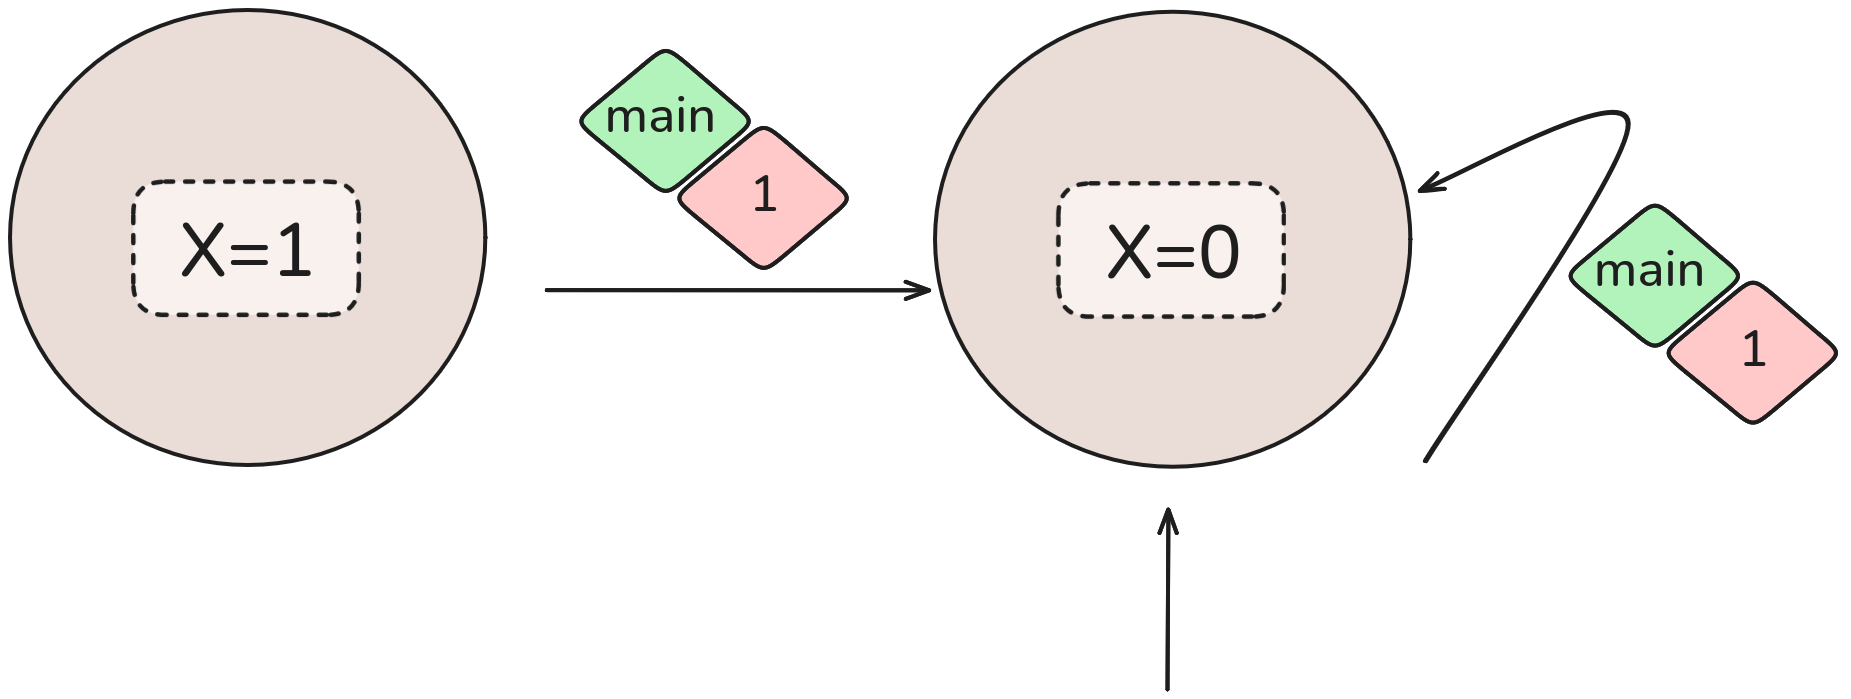
\includegraphics[width=0.5\textwidth,trim=0 0 0 0,clip]{plots/code_2_NFA.png}
	\caption{NFA for serialized executions of Listing~\ref{lst:MotivatingExample2NonSer} program.}
	\label{fig:code2ExampleNFA}
\end{figure}

\paragraph{Petri Net Extraction.}

Finally, the NS gives rise to to generate the following Petri Net, encoding all possible interleavings of our program:

\begin{figure}[!htbp]
	\centering
	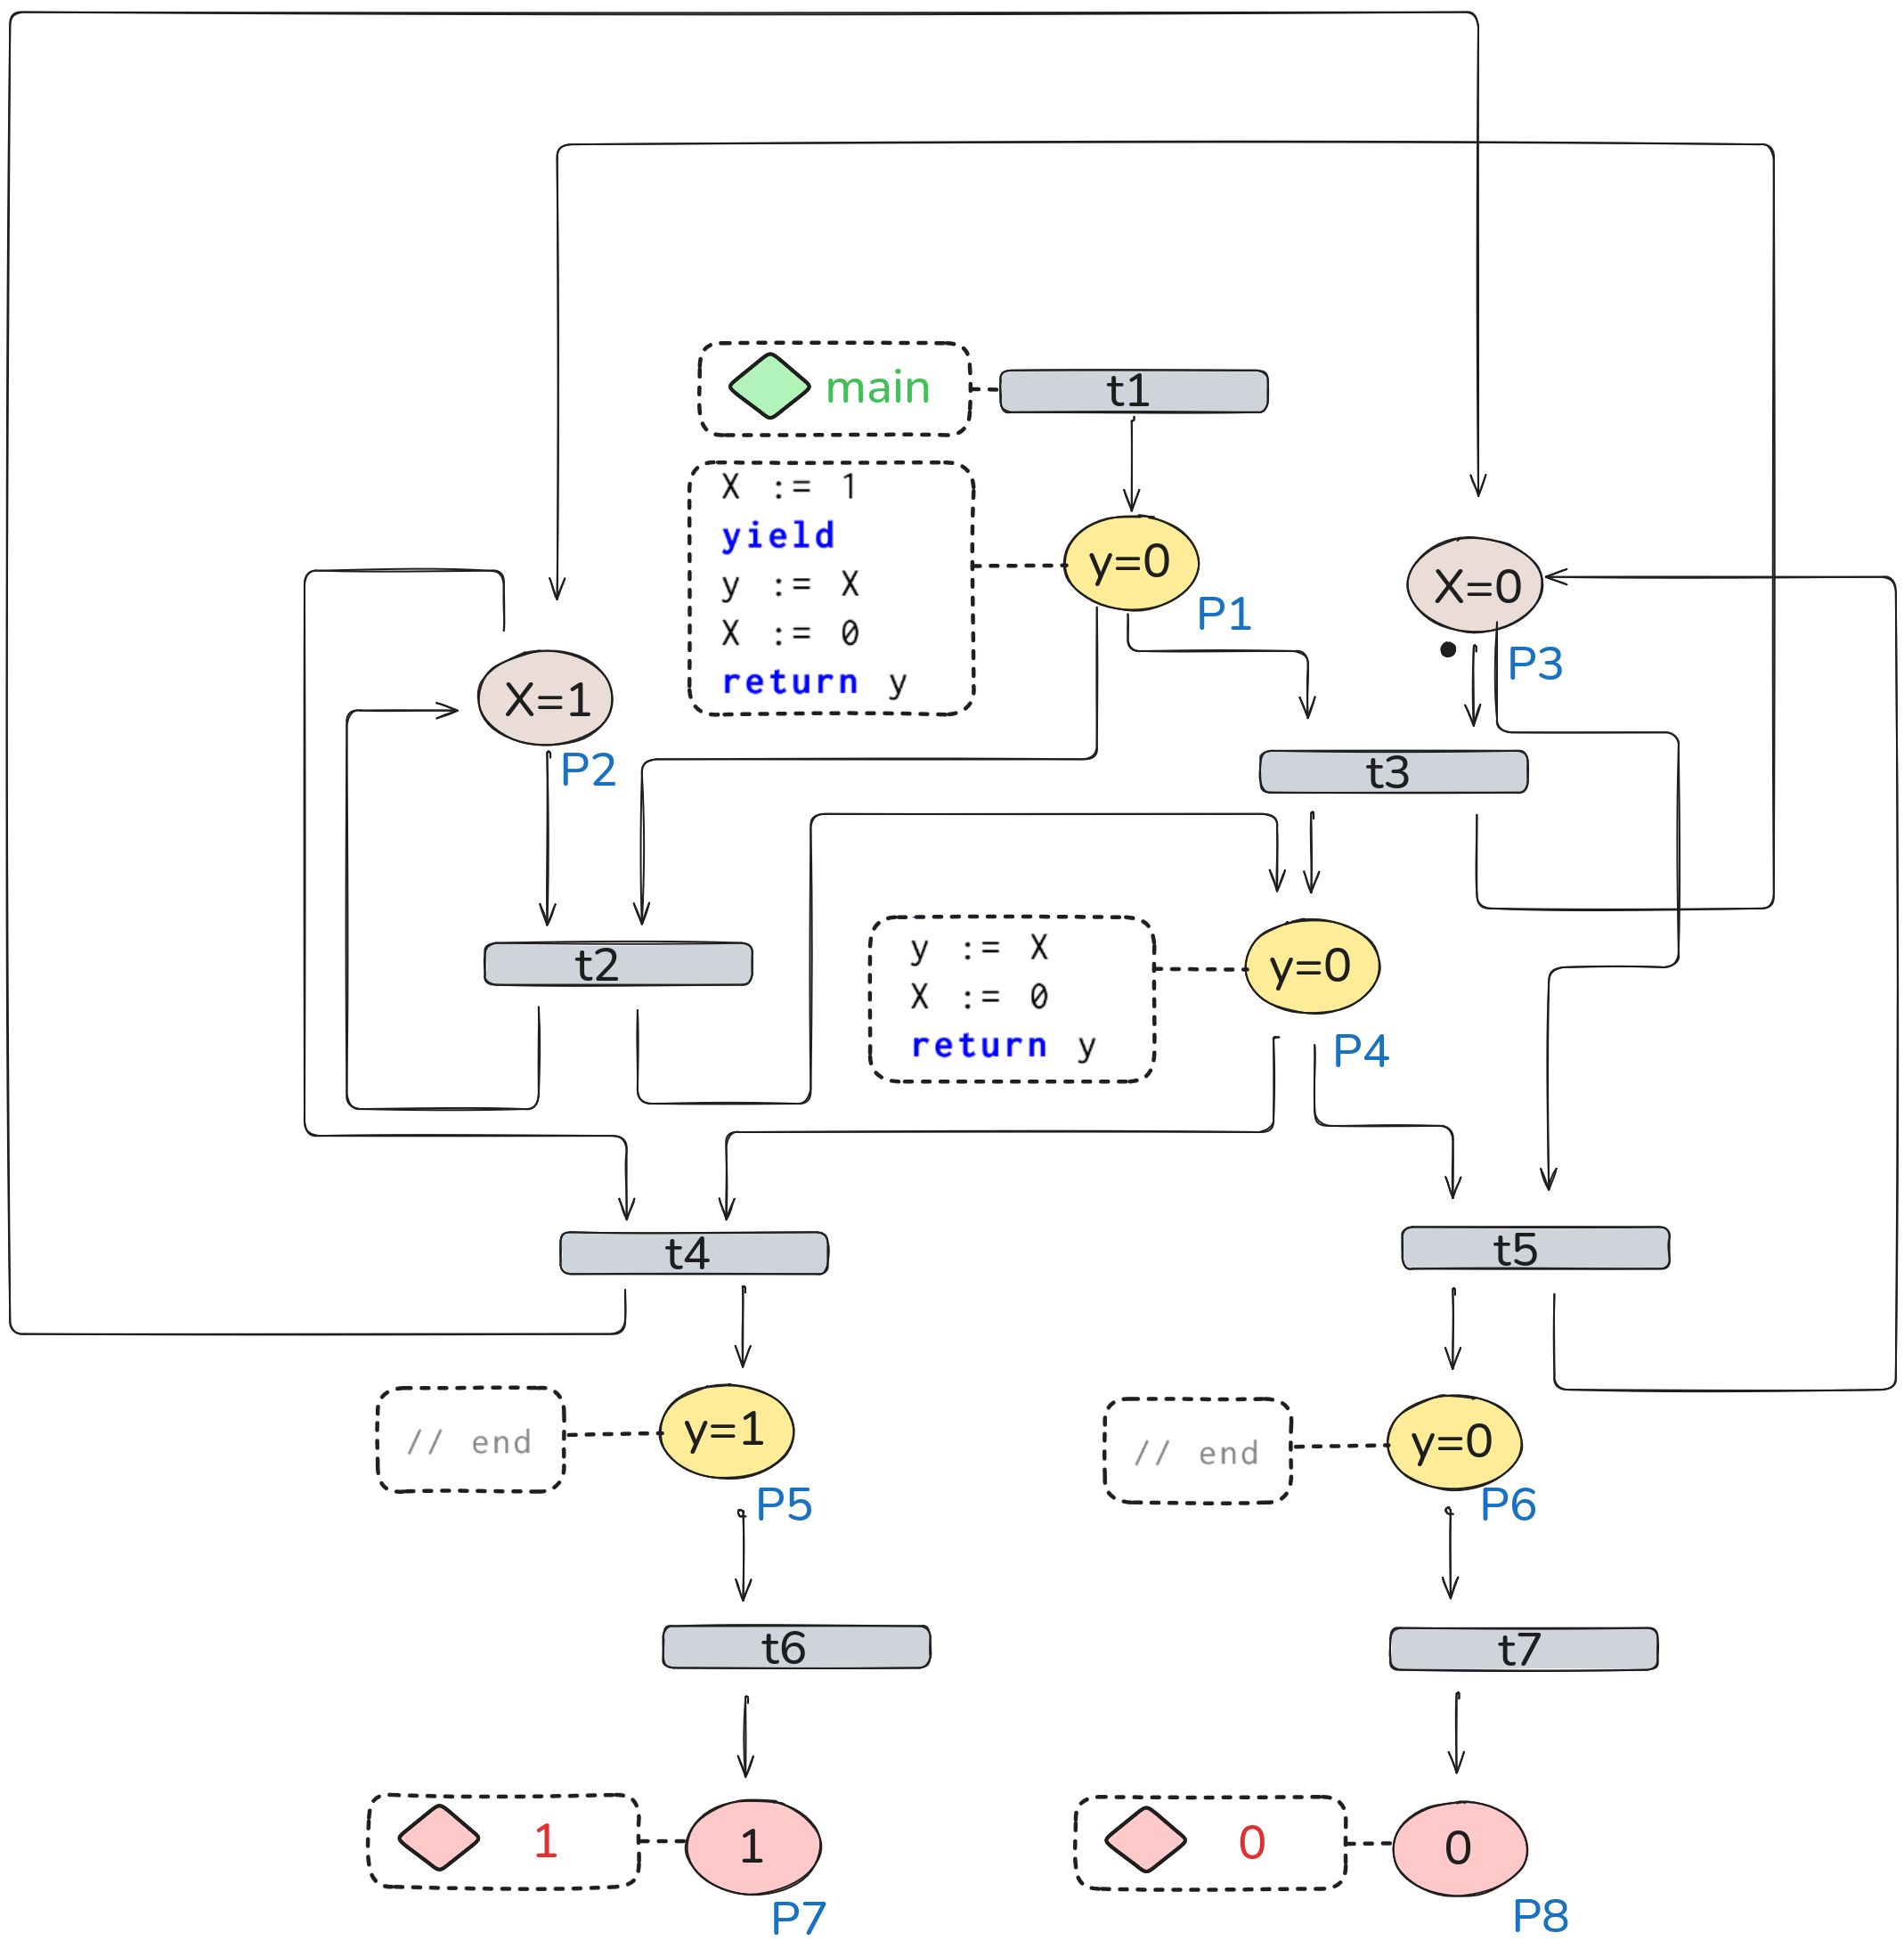
\includegraphics[width=0.7\textwidth]{plots/code_2_PN_with_annotation.png}
	\caption{Petri Net for interleaving executions of Listing~\ref{lst:MotivatingExample2NonSer} program. Note that there doesn't exist any valid firing sequence that can reach place $P_8$, representing a response of {\color{red}$\blacklozenge_0$}.}
	\label{fig:code2ExamplePN}
\end{figure}

The places represent the $\delta$ transitions of our NS --- encoding either a ``step'' of our program, or spawning a request ($t_1$, which  corresponds to spawning request {\color{ForestGreen}$\blacklozenge_\text{main}$}), or returning a response, e.g. transitions $t_6,t_7$ that corresponds to outputting responses {\color{red}$\blacklozenge_1$},{\color{red}$\blacklozenge_0$}.
%
Some places (\textcolor{blue}{$P_2$},\textcolor{blue}{$P_3$}) corresponds to the global state, while others ($P_1,P_4,P_5,P_6$) corresponds to the local state of an in-flight request.
%
Each token corresponds to a single request packet, or (in the case of the global-variable-encoding places), to the global state of the program.

\paragraph{Counterexample Extraction.}

Regarding the aforementioned program, we automatically generate the following reachability query for the Petri net of Figure~\ref{fig:code1ExamplePN} (which, if satisfiable, indicates the program is not serializable):

\guy{Nicolas could you fix the "exists Marking M"? How do you suggest we formulize?}

\[
\exists\,M.\; 
P_1 = 0 \wedge 
\textcolor{blue}{P_2} \ge 0 \wedge \textcolor{blue}{P_3} \ge 0  \wedge P_4 = 0
\wedge P_5 = 0 \wedge P_6 = 0 \wedge \textcolor{red}{P_7} = 0 \wedge \textcolor{red}{P_8} \ge 1.
\]
This asserts the existence of a marking with no tokens on $P_1,P_4,P_5,P_6$,$\textcolor{red}{P_7}$, at least one token on $\textcolor{red}{P_8}$, and arbitrary tokens on $\textcolor{blue}{P_2},\textcolor{blue}{P_3}$.  In fact, the target marking
\[
M^* = \{\textcolor{blue}{P_3}(1),\;\textcolor{red}{P_7}(1),\;\textcolor{red}{P_8}(1)\}
\]
is reachable.  Table~\ref{tab:PetriNetFiringCounterexample} lists a firing sequence that leads to $M^*$.





\begin{table}[H]
	\centering
	\label{tab:reach-seq}
	\begin{tabular}{c l c c c c c c}
		\toprule
		\textbf{Step} 
		& \textbf{Firing} 
		& \multicolumn{3}{c}{\textbf{Marking (after firing)}} 
		& \multicolumn{3}{c}{\textbf{Description (after firing)}} \\
		\cmidrule(lr){3-5} \cmidrule(lr){6-8}
		& 
		& \textbf{Global} 
		& \textbf{Local} 
		& \textbf{Responses} 
		& \textbf{Global state} 
		& \textbf{In-flight packets} 
		& \textbf{Responses} \\
		\midrule
		0 & --                                  
		& {\color{blue}$P_3$(1)}                  
		& --                                    
		& --                                    
		& {\color{blue}[X=0]}                   
		& --                          
		& --                                    \\
		1 & $t_1$ 
		& {\color{blue}$P_3$(1)}                  
		& $P_1$(1)                                
		& --                                    
		& {\color{blue}[X=0]}                   
		& {\color{ForestGreen}$\blacklozenge_\text{main}$} 
		& --                                    \\
		2 & $t_1$ 
		& {\color{blue}$P_3$(1)}                  
		& $P_1$(2)                                
		& --                                    
		& {\color{blue}[X=0]}                   
		& {\color{ForestGreen}$\blacklozenge_\text{main}$}, {\color{ForestGreen}$\blacklozenge_\text{main}$}  
		& --                                    \\
		3 & $t_3$                                  
		& {\color{blue}$P_2$(1)}                  
		& $P_1$(1),$P_4$(1)                          
		& --                                   
		&                                    {\color{blue}[X=1]}    
		&                                    {\color{black}$\blacklozenge_\text{until yield}$}, {\color{ForestGreen}$\blacklozenge_\text{main}$}   
		& --                                    \\
		4 & $t_2$                                  
		& {\color{blue}$P_2$(1)}                  
		& $P_4$(2)                                
		& --                                    
		&                                    {\color{blue}[X=1]}    
		&                                    {\color{black}$\blacklozenge_\text{until yield}$}, {\color{black}$\blacklozenge_\text{until yield}$}   
		& --                                    \\
		5 & $t_4$                                  
		& {\color{blue}$P_3$(1)}                  
		& $P_5$(1),$P_4$(1)                          
		& --                                    
		&                                   {\color{blue}[X=0]}     
		&                                    {\color{black}$\blacklozenge_\text{after yield}$}, {\color{black}$\blacklozenge_\text{until yield}$}   
		& --                                    \\
		6 & $t_6$                     
		& {\color{blue}$P_3$(1)}                  
		& $P_4$(1)                                
		& {\color{red}$P_7$(1)}                    
		&                                      	{\color{blue}[X=0]}  
		&                                    {\color{black}$\blacklozenge_\text{until yield}$}   
		&                                   {\color{red}$\blacklozenge_1$}     \\
		7 & $t_5$                                  
		& {\color{blue}$P_3$(1)}                  
		& $P_6$(1)                                
		& {\color{red}$P_7$(1)}                    
		&                                   {\color{blue}[X=0]}    
		&                                    {\color{black}$\blacklozenge_\text{after yield}$}      
		&                                   {\color{red}$\blacklozenge_1$}        \\
		8 & $t_7$                     
		& {\color{blue}$P_3$(1)}                                  
		& --                                    
		& {\color{red}$P_7$(1),\color{red}$P_8$(1)}    
		&                                   {\color{blue}[X=0]}    
		&                                   --    
		&                                   {\color{red}$\blacklozenge_0$}, {\color{red}$\blacklozenge_1$}       \\
		\bottomrule
	\end{tabular}
	\caption{Firing sequence reaching the target marking $M^*$. The marking $P_i(n_j)$ indicates that there are $n_j$ tokens on place $P_i$. The initial marking has a single token in place $P_3$ encoding the initial global state.}
	\label{tab:PetriNetFiringCounterexample}
\end{table}

%\newpage

\subsection{Example: Serializable Program}
\label{subsec:ns-serializable}

Now, we observe again the adjusted program with locks (as previously described in Listing~\ref{lst:MotivatingExample3Ser}).
%
Due to space limitations, we relegate figures of the corresponding Network System, Serailizability NFA, and Interleaving Petri Net to Appendix~\ref{appendix:MoreNsExamples}, and focus on the serializability proof certificate.

Non-serializability corresponds to the Petri Net (in Fig.~\ref{fig:code3ExamplePN}) being able to reach the following marking:

\[
\exists\,M.\; \textcolor{blue}
P_1 = 0 \wedge 
{P_2} \ge 0 \wedge \textcolor{blue}{P_3} \ge 0  \wedge P_4 = 0
\wedge P_5 = 0 \wedge P_6 = 0 \wedge \textcolor{red}{P_7} = 0 \wedge \textcolor{red}{P_8} \ge 1.
\]


Note that this happened to be the exact same property as encoding non-serializability in the previous example, however, the Petri Net places $(P_1,\ldots,P_8)$ encode different states that correspond to the updated program. For example, now each place in the PN that encodes a global state accounts for two global variables, $X$ and $L$. 
%
Furthermore, unlike the previous example, this semilinear encoding (of non serializability) is \textit{unreachable}, as witness by the following inductive invariant that we produce.


\[
\begin{aligned}
	&(P_{1},\textcolor{blue}{P_{2}},\textcolor{blue}{P_{3}},P_{4},P_{5},P_{6},\textcolor{red}{P_{7}},\textcolor{red}{P_{8}})
	\;\mapsto\;\\
	&\quad
	\exists\,e_{0},\dots,e_{5}\ge0.\;
	\Bigl(
	e_{2}-e_{1}+\textcolor{blue}{P_{3}}-1=0\;\land\;
	e_{2}+P_{1}-e_{5}=0\;\land\;
	P_{5}-e_{1}+e_{4}=0\;\land\\
	&\qquad\quad
	-\,e_{4}+\textcolor{red}{P_{7}}=0\;\land\;
	P_{6}+e_{3}-e_{0}=0\;\land\;
	\textcolor{red}{P_{8}}-e_{3}=0\;\land\\
	&\qquad\quad
	-\,e_{2}+e_{1}+e_{0}+P_{4}=0\;\land\;
	-\,e_{2}+e_{1}+\textcolor{blue}{P_{2}}=0
	\Bigr)
	\;\land\;
	\bigl(P_{4}-1\ge0\;\lor\;\textcolor{blue}{P_{3}}-1\ge0\bigr).
\end{aligned}
\]


We then revert this invariant to match our Network System, and project it to request/response pairs of the network system.
%
We get the following inductive invariants for each of the two (reachable) global states:

\begin{proof}
	
	\medskip\noindent
	For global state \textcolor{blue}{[L=0,X=0]}
	the projected invariant is:
	\[
	\bigl(\,\text{\color{ForestGreen}$\blacklozenge_{\text{main}}$}/\text{\color{red}$\blacklozenge_{0}$},\;
	\text{\color{ForestGreen}$\blacklozenge_{\text{main}}$}/\text{\color{red}$\blacklozenge_{1}$}\bigr)
	\;\mapsto\;
	\exists\,e_{0},\dots,e_{5}\ge0.\;
	\begin{aligned}[t]
		& e_{2}-e_{1}=0,\quad
		e_{2}-e_{5}=0,\quad
		-e_{1}+e_{4}=0,\\
		& -e_{4}+\bigl(\text{\color{ForestGreen}$\blacklozenge_{\text{main}}$}/\text{\color{red}$\blacklozenge_{1}$}\bigr)=0,\quad
		-e_{0}+e_{3}=0,\quad
		-e_{3}+\bigl(\text{\color{ForestGreen}$\blacklozenge_{\text{main}}$}/\text{\color{red}$\blacklozenge_{0}$}\bigr)=0,\\
		& -e_{2}+e_{1}+e_{0}=0,\quad
		-e_{2}+e_{1}=0.
	\end{aligned}
	\]
	From these:
	\[
	e_{1}=e_{2}=e_{4}=e_{5}=(\;
	\text{\color{ForestGreen}$\blacklozenge_{\text{main}}$}/\text{\color{red}$\blacklozenge_{1}$}),\;
	e_{0}=e_{3}=
	(\text{\color{ForestGreen}$\blacklozenge_{\text{main}}$}/\text{\color{red}$\blacklozenge_{0}$}),
	\]
	and
	\[
	-e_{2}+e_{1}+e_{0}=0\;\Longrightarrow\;e_{0}=0.
	\]
	Thus
	\[
	(	\text{\color{ForestGreen}$\blacklozenge_{\text{main}}$}/\text{\color{red}$\blacklozenge_{0}$})
	=0,
	\]
	indicating that  (\(\text{\color{ForestGreen}$\blacklozenge_{\text{main}}$}/\text{\color{red}$\blacklozenge_{0}$}\)) cannot be attained from the global state
	\textcolor{blue}{[L=0,X=0]}.
	
	\medskip\noindent
	In the second case, for the global state \textcolor{blue}{[L=1,X=1]}.
	The projected invariant is:
	
	
	\[
	\bigl(\,\text{\color{ForestGreen}$\blacklozenge_{\text{main}}$}/\text{\color{red}$\blacklozenge_{0}$},\;
	\text{\color{ForestGreen}$\blacklozenge_{\text{main}}$}/\text{\color{red}$\blacklozenge_{1}$}\bigr)
	\;\mapsto\;
	\exists\,e_{0},\dots,e_{5}.\;\bot,
	\]
	which is unsatisfiable.  Hence, no completed‐request pair, and in particular no (\(\text{\color{ForestGreen}$\blacklozenge_{\text{main}}$}/\text{\color{red}$\blacklozenge_{0}$}\)) pair can be produced from this state via a non-serializable execution.
	\guy{Jules is this part correct?}
	
	\medskip\noindent
	\textbf{Conclusion.}
	In all reachable states
	it holds that there cannot be any request/response pair of type
	(	$	\text{\color{ForestGreen}$\blacklozenge_{\text{main}}$}/\text{\color{red}$\blacklozenge_{0}$}
	$).
	%
	Furthermore, this indicates that the only attainable request/response pairs are of the form 	($	\text{\color{ForestGreen}$\blacklozenge_{\text{main}}$}/\text{\color{red}$\blacklozenge_{1}$})
	$, which are included in the language of of NFA for serial executions. Thus, this program is serializable.
	%
	We further show (in Appendix~\ref{appendix:InductiveInvariantExample}) that these invariants are \textit{inductive}: they encompass the system’s initial state and, once satisfied, remain true for all subsequent executions.
\end{proof}



%\newpage


\subsection{Time/Space Complexity}

\todo{consult with Jules}


\subsection{Optimizations}
\label{sec:optimizations}

\todo{check}

We apply four optimizations to the base algorithm to control intermediate blow‐up in the size of both the PN and the constructed semilinear set.

\paragraph{(1) Bidirectional pruning.}  
\guy{should we reformulate this like in Appendix D?}
Let \(N=(P,T,\mathsf{pre},\mathsf{post},M_0)\) and let \(\mathit{Tgt}\subseteq P\) be the ``nonzero” places extracted from the Presburger constraints.  Define the flip of \(N\), \(\overline N\), by swapping \(\mathsf{pre}\) and \(\mathsf{post}\).  We compute a decreasing sequence of transition‐sets
\[
T^{(0)} = T,\qquad
\begin{aligned}
	R_{\mathrm{fw}}^{(k)} &= \{\,t\in T^{(k)} \mid \exists\,M_0\xrightarrow{*}M\text{ in }N\text{ enabling }t\},\\
	R_{\mathrm{bw}}^{(k)} &= \{\,t\in T^{(k)} \mid \exists\,M\xrightarrow{*}M'\text{ in }\overline N\text{ with }M'(p)>0\;(p\in\mathit{Tgt})\},\\
	T^{(k+1)} &= R_{\mathrm{fw}}^{(k)} \;\cap\; R_{\mathrm{bw}}^{(k)}.
\end{aligned}
\]
We repeat until \(T^{(k+1)}=T^{(k)}\).  In each iteration we record
\(\Delta_{\mathrm{fw}}^{(k)}=R_{\mathrm{fw}}^{(k-1)}\setminus R_{\mathrm{fw}}^{(k)}\)
and
\(\Delta_{\mathrm{bw}}^{(k)}=R_{\mathrm{bw}}^{(k-1)}\setminus R_{\mathrm{bw}}^{(k)}\).
%
This optimization allows to significantly prune the Petri Net while still over-approximating all reachable markings (see the proof in Appendix~\ref{appendix:BidirectionalProof}).

\paragraph{(2) Semilinear‐set pruning.}  
Recall a semilinear set is \(S=\bigcup_{i=1}^m L_i\) with
\(\displaystyle L_i=\{\,b_i+\sum_{p\in P_i}n_p\,p\mid n_p\in\mathbb N\}\).  
%
We replace each period‐basis \(P_i\) by
\[
P_i \;:=\;\{\,p\in P_i \mid p\notin\mathsf{Span}(P_i\setminus\{p\})\},
\]
dropping any ``redundant” period, and remove any \(L_j\subseteq L_i\) for \(i\neq j\), iterating to a fixpoint so no two components subsume one another.

\paragraph{(3) Generating fewer constraints.}  
Let $\mathrm{comp}(S)=\{L_1,\dots,L_m\}$ 
be the multiset of linear components of the semilinear set 
\(\displaystyle S=\bigcup_{i=1}^m L_i\), where each 
\(\;L_i=b_i+\langle P_i\rangle\) with \(b_i\in\mathbb N^d\) and 
\(P_i\subseteq\mathbb N^d\).  Define the pruning operator
\[
\mathrm{new}(\mathcal C)
\;=\;
\bigcup\bigl\{\,L\in\mathcal C \;\bigm|\;\nexists\,L'\in\mathcal C\setminus\{L\}:\;L'\subsetneq L\bigr\},
\]
which removes any component strictly containing another.  
%
\guy{Nicolas is it clear we mean that we fix their semilinear "meaning" of the regex operations? For example, + is union etc..}
Then, we replace the naïve semilinear‐set operations by
\[
S\;+\;T
\;=\;
\mathrm{new}\bigl(\mathrm{comp}(S)\,\cup\,\mathrm{comp}(T)\bigr),
\]
\[
S\;\cdot\;T
\;=\;
\mathrm{new}\Bigl(\{\,L_i\cdot L'_j \mid L_i\in\mathrm{comp}(S),\;L'_j\in\mathrm{comp}(T)\}\Bigr),
\]
where for
\(\;L_i=b_i+\langle P_i\rangle,\;L'_j=b'_j+\langle P'_j\rangle\) we set
$
L_i\cdot L'_j
=\;(b_i+b'_j)\;+\;\langle\,P_i\cup P'_j\,\rangle.
$
Finally, for Kleene‐star and plus on the regex side one similarly applies
\(\mathrm{new}(\cdot)\) to the collection of ``folded” components instead of
building all intermediate ones:
\[
S^*
=\mathrm{new}\Bigl(\bigcup_{k\ge0}\bigl(\mathrm{comp}(S)\bigr)^k\Bigr),
\qquad
S^+
=S\cdot S^*.
\]

\paragraph{(4) Strategic Kleene elimination order.}  
When converting an NFA \(\mathcal A=(Q,\Sigma,\delta,q_0,F)\) to a regex by repeated state‐elimination, then, instead of choosing an arbitrary state $q\in Q'$, we pick the next state
\[
q^* = 
	\arg\min_{q\in Q'}\bigl(|\delta_{\mathrm{in}}(q)|+|\delta_{\mathrm{out}}(q)|\bigr)
\]


where \(Q'\subseteq Q\) are the states remaining to be eliminated.  This heuristic keeps the intermediate regex small.


%\newpage

\section{Implementation}
\label{sec:implementation}

The implementation..

\begin{enumerate}
    \item The extra things we did to make the thing actually run
    \item Code architecture
    \item Optimizations
\end{enumerate}

\newpage
\section{Evaluation}
\label{sec:evaluation}

\begin{enumerate}
    \item Benchmarks (describe our benchmarks)
    \item Results (total time, split out SMPT time from our rust code time)
    \item Analysis of optimizations (how much time they save, petri net sizes, semilinear set sizes)
    \item Limitations (examples we cannot solve, future work that would help)
\end{enumerate}





\begin{tabular}{l c c c c}
	\toprule
	& \multicolumn{2}{c}{num components} & \multicolumn{2}{c}{periods per component} \\
	\cmidrule(lr){2-3} \cmidrule(lr){4-5}
	& mean & max & mean & max \\
	\midrule
	baseline (all optimizations)    &  3.28 (+0\%) &  22.00 (+0\%) & 1.36 (+0\%) &  4.00 (+0\%) \\
	baseline - remove\_redundant & 10.24 (+6.97\%) & 194 (+172\%)& \textbf{1.79 (+0.43\%)} & 11 (+7\%) \\
	baseline - generate\_less    &\textbf{782.38 (+779.10\%)}&\textbf{20484 (+20462\%)}&1.65 (+0.29\%)& \textbf{15 (+11\%)} \\
	baseline - smart\_order      &  3.36 (+0.09\%) &  22.00 (+0\%) & 1.38 (+0.02\%) &  4.00 (+0\%) \\
	\bottomrule
\end{tabular}
\textbf{The Table compares experiment running with a 30 second timeout}



\newpage
\section{Related Work}
\label{sec:relatedWork}

% from the CAV-2010 Vafeiadis paper (+ some other papers in our slack RW thread):
%
%1. model checking techniques - find violations, but do not prove correctness as they work on finite-state systems
%
%2. static (and specifically, shape) analysis techniques (sometimes) work on unbounded threads but ,any of these require linearization points (annotated manually or automatically). Also, a ``failed'' proof can indicate incorrect linearization.
%
%3. manual verification efforts

\subsection{Notions of serializability.}
\label{sec:related:notions-of-serializability}

Serializability (also termed 
\textit{atomicity}) was first formalized by Eswaran et al.~\cite{EsGrKoTr76} as 
a 
correctness condition for concurrent transaction execution. 
Their work also introduced what was later referred to as \textit{conflict 
serializability}, a stricter variant that requires equivalence to a serial 
schedule solely by reordering non-conflicting operations (e.g., two reads by 
different threads). 
%
\textit{Strict serializability} (a.k.a. SSR~\cite{Pa79}) is a stronger 
consistency 
notion in which an execution need not only be serializable but also respects 
the real-time ordering of the transactions, i.e., it is not enough for the 
interleaving to be equivalent to a serial one, but the serial execution must 
also preserve the ordering of the transactions.
%
%Strict serializability:
%
%Guerraoui et al.~\cite{GuHeJoSi08} present a algorithm for model checking 
%strict serializability fro two threads. The work was later 
%extended~\cite{GuHeSi11}, to include a manual proof for an arbitrary number of 
%threads.
%
%Konig and Wehrheim recently proved that it is possible to decide whether 
%all executions of a program are strictly serializable, given that the 
%transactions are live~\cite{KoWe21}.
%
Herlihy and Wing~\cite{HeWe87, HeWi90} defined \textit{Linearizability} as a 
similar notion to that of serializability, but adapted from transactional 
programs 
to concurrent data structures. In this setting, a linearizable data structure 
is one for which every concurrent execution 
with any operations manipulating it, appearing as if the operations occurred 
atomically, while respecting real-time ordering and obeying the object's 
specification. 
%
Equivalently, this can also be viewed as a case of strict serializability in 
which each transaction consists of a single action, operating on a single 
concurrent object~\cite{WaSt06a}.
%
Due to the similarity between serializability and linearizability, we cover 
related work pertaining to both notions.
%
Zhang et al.~\cite{ZhChWa13} relaxed the notion of linearizability to 
\textit{quasi 
linearizability}, and put forth a method to identify violations thereof in 
concurrent data structures.
%
Rastogi et al.~\cite{RaMeBrKoSi93} introduced the notion of 
\textit{predicate-wise serializability} (PWSR), which preserves database 
invariants 
while permitting non-atomic transactions.
%
Other non-serializability-related notions focus on weaker consistency models, 
and include Lamport’s \textit{causal 
consistency}~\cite{La78}, which was later generalized to shared 
memory~\cite{AhNeBuKoHu95} 
and implemented in systems like 
COPS~\cite{LlFrKaAn11}, and inspiring extensive research on model checking and 
complexity analysis~\cite{BoEnGuHa17,ZeBiBoEnEr19,LaBo20}. 


\subsection{Deciding serializability and linearizability}

\subsubsection{Theoretical Results}
%
The \textit{membership problem} of serializability, is deciding whether a 
specific interleaving is serializable. This has been proven to be 
\texttt{NP}-complete 
by Papadimitriou~\cite{Pa79}, a result that was later extended~\cite{BiEn19} to 
other consistency models.
Regarding linearizability, the easier, membership problem is 
\texttt{NP}-complete in 
general, as proven by Gibbons and Korach~\cite{GiKo97}. Their result was later 
extended to \textit{collections}~\cite{EmEn18}.
%\guy{Mark could you check EmEn18?}
%
The \textit{correctness problem} on the other hand, is much harder, and 
pertains to deciding whether \textit{all} executions of a program are 
serializable.
%
While the correctness problem of linearizability is in 
\texttt{EXPSPACE}~\cite{AlMcPe96} when bounding the number of threads, 
 Bouajjani et al.~\cite{BoEmEnHa13} proved that it is undecidable otherwise. 
 The authors also prove that the correctness problem of 
linearizability becomes decidable on the fragment of finite-barrier programs. 
As serializability can be viewed as a case in which there are no barriers, this 
implies that serializability membership is in fact decidable. 
%
In follow-up work, Bouajjani et al. prove that linearizability is decidable 
also 
in the unbounded case for specific abstract state types~\cite{BoEmEnHa18}, in 
which the authors rely on checking coverability in a Vector Addition System 
with States (VASS), which was proven to be in \texttt{EXPSPACE}~\cite{Ra78}.
%
Our work can be viewed as the first tool to implement serializability proofs, 
building upon the theoretical algorithm proposed by Bouajjani et 
al.~\cite{BoEmEnHa13}. While our setting differs from theirs in various aspects 
(e.g., we derive 
the serial specification directly from the program and provide a correctness 
proof; our setting is a transactional distributed system while their setting pertains to a single concurrent object, etc.), the core connection makes our work an implementation of their approach 
in spirit. However, despite the theoretical foundation, the implementation 
itself is the key novelty—translating their algorithm into a practical, 
scalable tool required significant advancements. The process was highly 
non-trivial, demanding various optimizations such as automatic invariant 
inference, automaton minimization, and additional techniques to handle 
unbounded systems efficiently. To the best of our knowledge, ours is the first 
tool capable of verifying serializability in unbounded domains.
%
While these contributions represent significant advances, to our knowledge, our 
work is the first to:
(i) Decide serializability universally --- \textit{considering all executions} 
purely through program semantics and final states, independent of read/write 
conflicts; 
(ii) Support \textit{unbounded} transaction systems; and
(iii) Provide a complete end-to-end implementation.



\subsubsection{Model checking and runtime verification}

In a series of papers, Wang and Stoller put forth runtime techniques for 
detecting violations to serializability~\cite{WaSt06a} as well as fragments of 
serializability such 
as conflict serializability and view-serializability~\cite{WaSt06b}. They do so 
by  checking whether a given execution can be recombined to generate 
non-serializable executions.
%
The expressive Temporal Logic of Actions (TLA)~\cite{La94} is used to encode a 
formal specification that validates whether only serializable executions (or 
conflict-serializable~\cite{CoOlPnTuZu07}) always occur. 
While TLA can naturally encode ``real'' serializability (based on final-state 
equivalence), existing TLA-based approaches~\cite{SoVaVi20, Ho24} remain 
limited to bounded transaction systems. This limitation stems from TLA/TLA+ 
model checkers like \texttt{TLC} and \texttt{Apalache}~\cite{YuMaLa99, 
KoKuTr19}, which require 
finite-state verification and cannot handle unbounded transaction counts.
%
\texttt{Line-up}~\cite{BuDeMuTa10} (built on the \texttt{CHESS} model 
checker~\cite{MuQaBaBaNaNe08}) includes a heuristic-driven technique that 
searches for violations of linearizability by enumerating all possible 
serializations. Similar to spirit is \texttt{LinTSO}~\cite{BuGoMuYa12} which 
search for 
linearizability violations in the Total Store
Order (TSO) weak memory model.
%
\texttt{Violat}~\cite{EmEn19} is a tool that generates tests to identify 
linearizability violations, by 
enumeration linearizations efficiently, per program schema (instead of per 
execution, as in~\cite{BuDeMuTa10}).This follows the authors' previous runtime verification technique~\cite{EmEn18}, which enumerates minimal visibility relations.
%
Additional model checking techniques were proposed by Burnim et 
al.~\cite{BuNeSe11}, which are similar to Line-up~\cite{BuDeMuTa10} but based 
on leveraging bridge predicates~\cite{BuSe09}. 
%
Liu et al.~\cite{LiChLiSuZhDo12} build upon \texttt{PAT}~\cite{SuLuDoPa09} 
(also used 
in~\cite{LiChLiSu09, Zh11}) and verify linearizability through the lens of 
refinement checking optimization, for a finite number of threads.
%
%\guy{Mark, could you please check LiChLiSu09,Zh11}
%
Recently, Golovin et al.~\cite{GoKoVa25} presented \texttt{RELINCHE}, a model 
checker for bounded-linearizability, in which a predefined number of operations 
can be invoked invoked.
%
Other automatic linearizability checking tools include the \texttt{CDSSpec} 
specification checker under the C/C++ 11 memory model, and 
\texttt{Lincheck}~\cite{KoDeSoTsAl23} for verifying linearizability in JVM by 
Ou and 
Demsky~\cite{OuDe17}. 
%
Burckhardt et al.~\cite{BuAlMa07} employ a SAT solver and check for 
linearizability violations of specific client programs.
%
We also note the symbolic-reasoning-based (incomplete) approach by Emmi et 
al.~\cite{EmEnHa15} to identify violations of \textit{observational refinement} 
--- a property equivalent to linearizability in some settings~\cite{FiOhRiYa10, 
	BoEmCoHa15}.
%
As far as we are aware, unlike our algorithm, none of these tools afford 
complete coverage for the case of unbounded threads.
%
Other model checking techniques (e.g.,~\cite{Fl04}) rely on specifying 
\textit{linearization points} (a.k.a. commit points), i.e., points in which the 
event occurs logically. We note 
that identifying all such points can be quite challenging~\cite{VeYaYo09}.
%
These include the work of Vechev et al.~\cite{VeYaYo09}, built upon 
\texttt{SPIN}~\cite{Ho97}, and extending the authors' \texttt{PARGLIDER} 
tool~\cite{VeYa08}.~\footnote{Note that Vechev et al. can also apply their 
technique without linearization points, but solely on bounded executions.}



\subsubsection{Stataic analysis}

Static analysis techniques may prove linearizability for the 
bounded~\cite{AmRiReSaYa07, BeLeMaRaSa08, MaLeSaRaBe08} and unbounded 
cases~\cite{BeLeMaRaSa08, Va09, 
	Va10}, but typically rely on heuristics and the manual/automatic annotation 
	of 
linearization points. 
%
Lian and Feng~\cite{LiFe13} propose a sound program logic that can prove 
linearizability with non-fixed linearization points.
%
Other techniques that depend on linearization points 
include~\cite{OhRiVeYaYo10, ZhPeHa15, AbJoTr16}. 
%
%\guy{Mark can you take a look at Va10, LiFe13, and ZhPeHa15?}
%
We note that both the model-checking techniques (e.g.,~\cite{CeRaZuChAl10}) and 
the static analysis techniques which rely on linearization points are 
inconclusive, as any failed proof can be due to incorrect annotation of the 
linearization points, as previously observed~\cite{BoEmCoHa15}.
%


\subsubsection{Manual proofs and results for specific data types}

Tasiran~\cite{Ta08} proved serializability of the \texttt{Bartok STM}, and 
Colvin et 
al.~\cite{CoGrLuMo06} prove that a list-based set algorithm is linearizable by 
simulating the observed behavior with input/output automata.
%
%\guy{Mark could you take a 2nd look at CoGrLuMo06? Not sure if this is 
%considered manual. One paper which I put in the slack channel mentioned that it 
%semiautomatically verifies linearizability of an implementation.}
%
Other methods demonstrate that in some cases, proofs can be simplified for specific data structure to which certain properties hold~\cite{BoEmEnMu17, FeEnMoRiSh18}.
%
Additional verification attempts of linearizability have been presented both 
with (e.g.~\cite{CoGrLuMo06}) and without (e.g.~\cite{DoGrLuMo04}) the use of 
proof assistants.
%
Linearizability has also been proven for specific data types. For example. 
Wing and Gong~\cite{WiGo93} prove it for  (unbounded) FIFO queues, (unbounded) 
priority queues and other data structures. Chakraborty et al.~\cite{ChHeSeVa15} 
later provided a method for checking linearizability of queue-based algorithms, 
without the use of linearization points. Cern{\`y} et al.~\cite{CeRaZuChAl10} 
present \texttt{CoLT}, a model checker for linearizability of singly-linked 
heap-based 
objects. However, their approach is complete only with regard to a bounded 
number of threads. 
%
Bouajjani et al.~\cite{BoEnWa17} present a recursive algorithm for identifying 
linearizability violations in priority queues (based on register automata), in 
a method similar to the one for finding linearizability violations in stacks 
and (regular) queues~\cite{BoEmEnHa18}.
%


\subsubsection{Additional approaches}

%
Some methods combine multiple approaches, e.g., Shacham et 
al.~\cite{ShBrAiSaVeYa11} use dynamic analysis to identify 
violations of linearizability in concurrent data structures, and combine it 
with a manual proof when their technique did not find a violation.
%
Other techniques attempt to generate tests for linearizability~\cite{WiGo93, 
PrGr12, PrGr13, EmEn17}. For example, 
Lowe~\cite{Lo17} presents a testing framework for linearizability by randomly 
generating histories and subsequently testing if they are 
linearizable.
%
There has also been ample research in technique for linearizability  and simplifying proofs for data structures pertaining ~\cite{BoEmEnMu17, FeEnMoRiSh18, EnKo24} 
%
Other techniques for linearizability proof include the use of theorem provers, 
e.g.~\cite{CoDoGr05, DeScWe11} and proof assistance techniques~\cite{EnKo24}.
%
%\guy{Mark EnKo24 is the OOPSLA paper, is it legit to cite it as a proof assistance technique?} 
%Additional related work includes~\cite{BoEmEnMu17, FeEnMoRiSh18, EnKo24}.
%
%EnKo24: OOPSLA paper (Mark) trying to formalize and prove existing reduction techniques, and introduce a new abstraction for splitting linearizability checking scenarios (cases) and check if they covers all the checks. They don't actually check linearizability but say there it can help other checkers

%FeEnMoRiSh18 simplify proofs for some types of data structures

%BoEmEnMu17 also show that proof can be simplified sometimes 


\section{Deciding conflict serializability}

\subsubsection{Runtime enforcement}
Although conflict serializability is a more conservative measure than 
serializability, it is easier for database schedulers to enforce during 
runtime, either by \textit{pessimistic} locking approaches~\cite{BeHaGo87}, or 
\textit{optimistic} locking 
approaches~\cite{KuRo81, BuMo06}.
%
Both approaches ensure acyclicity in the conflict graph --- a necessary and 
sufficient condition for conflict serializability~\cite{SiMa10}. However, 
because these approaches \textit{ignore program semantics}, these may 
incorrectly reject executions that, although not conflict-serializable, are 
still valid serializable executions, i.e., have the same result as a serial 
execution. 
%
We note that the subject matter of this work is around the notion of (``real'') 
serializability, which takes 
into account the program semantics, and regards whether the final result of the 
program can be attained by a serial execution.
%

\subsubsection{Theoretical results}
From the theoretical perspective, Alur et al.~\cite{AlMcPe96} established that 
correctness problem for conflict serializability is decidable (and in 
\texttt{PSPACE}) 
for bounded transaction systems. Bouajjani et al.~\cite{BoEmEnHa13} later 
proved that decidability also holds in the unbounded case (and 
\texttt{EXPTIME}-complete). Their key insight reveals that while the conflict 
graph 
becomes infinite, cycle detection, and thus conflict serializability, is 
independent of the transaction count. 
%
%By modeling transactions via Vector Addition Systems (equivalent to Petri 
%Nets), they provide a finite framework for analyzing infinite behaviors. This 
%approach inspired our use of Petri Nets to capture Int(S).
%
\subsubsection{Approaches and techniques}

Various works focus on checking conflict serializability, e.g., Farzan and 
Mahusudan~\cite{FaMa08} present a monitoring-based decision procedure for 
conflict serializability of a bounded number of operations, and Flanagan et 
al.~\cite{FlFrYi08} present \texttt{Velodrome} --- a dynamic analyzer for 
conflict 
serializability. Additional dynamic approaches include~\cite{FlFr04, XuBoRa05, 
WaSt06a, CoOlPnTuZu07, EmMaMa10, SiMaWaGu11a} and others.
%
%Other works~\cite{XuBoRa05} have also put forth techniques to automatically 
%detect conflict-serializability violations.
%
Hatcliff et al.~\cite{HaRoDw04} demonstrate the use of the \texttt{Bogor} model 
checker~\cite{RoDwHa03} and check atomicity w.r.t. Liptopn's reduction theory 
of left/right movers~\cite{Li75} (which is reminiscent of 
conflict-serializability).
%
Elmas et al.~\cite{ElQaSeSuTa10} also use the notion of movers and present an 
(incomplete) technique to prove linearizability by iteratively rewriting an 
input program.
%
%\guy{Mark can you please check out ElQaSeSuTa10}
%
Nagar and Jagannathan~\cite{KaJa18} presented an 
automatic static analysis technique to find violations of conflict 
serializability.
%
Sinha et al.~\cite{SiMaWaGu11b} present a sound and incomplete predictive 
analysis technique for detecting violations of conflict serializability, 
following the previous work of Sinha and Malik~\cite{SiMa10} which put forth a 
runtime conflict serializability checker.
%
Von Praun and Gross~\cite{VoGr04} present an unsound static analysis technique 
for identifying potential atomicity violations. Additional static analysis 
techniques are based on type systems, e.g.~\cite{FlQa03, FlFrLiQa08}.
%
Brutschy et al.~\cite{BrDiMuVe17} present a dynamic analysis algorithm and a 
tool that checks whether a given program execution is conflict serializable, in 
an eventually consistent data store. In a follow-up work~\cite{BrDiMuVe18} 
further bridges these concepts by statically detecting 
non-(conflict)-serializable behaviors in causally consistent databases.
%
%Rinetzky et al.~\cite{RiBoRaSaYa} present a conservative static analysis 
%techniques for verifying view-serializability on specific program sub-types.
%
%\guy{Mark, please see my masked comment on RiBoRaSaYa. Do we need to mention 
%	them?}
%
We also note that conflict serializability has been studied in relation to weak 
memory models~\cite{EnFa16}.
%





\subsection{Petri Nets, VAS(S), Semilinear sets  \& Presburger arithmetic.}
\label{sec:related:petri}

In addition, our work builds on both theoretical and practical advances in 
Petri Net research~\cite{Mu89, Es96, Re12, EsNi24}. 
%The undecidability we prove 
%for equivalence of interleavings stems from Hack’s seminal result~\cite{Ha76, 
%HaThesis76} showing the undecidability of reachability set equivalence for 
%Petri Nets. This undecidability originates in a series of reductions from 
%Hilbert’s 10th problem, specifically the possibility of determining whether 
%there exists an integer root for Diophantine equations, a problem that was 
%later proven undecidable by Matijasēvič~\cite{Ma70}.
%%
%Jančar~\cite{Ja95} later provided an alternative proof to this undecidability 
%result, by showing that Petri Nets can simulate universal (and thus 
%undecidable) 2-counter Minsky machines~\cite{Mi67}. In addition, Jančar further 
%strengthened the original result by proving that undecidability holds even for 
%Petri nets with just five unbounded places.
%
%Furthermore, our approach also builds on 
as well as Petri Net reachability algorithms, 
which determine whether a given marking is attainable. While the solution is 
straightforward for bounded nets (through exhaustive enumeration), the solution 
for the unbounded case is highly nontrivial, and was first solved by 
Mayr~\cite{Ma81}, with subsequent improvements by Kosaraju~\cite{Ko82} and 
Lambert~\cite{La92}. Recent work~\cite{CzWo22} has also established this 
problem is \texttt{Ackermann}-complete, implying that, although decidable, it 
is practically infeasible to solve on large nets in the worst case.
%
These theoretical advances in Petri Net reachability have given rise to a 
plethora of practical tools, including \texttt{KReach}~\cite{DiLa20}, 
\texttt{DICER}~\cite{XiZhLi21}, \texttt{MARCIE}~\cite{HeRoSc13}, and others. 
%
Specifically, our implementation leverages \texttt{SMPT}~\cite{AmDa23}, a 
state-of-the-art Petri Net reachability tool that combines SMT-solving with 
structural invariants~\cite{AmBeDa21, AmDaHu22}. At a high level, SMPT 
formulates reachability as satisfiability queries (dispatched to the 
\texttt{Z3} 
solver~\cite{DeBj08}) while curtailing the search space~\footnote{As far as we 
aware, the only two sound reachability solvers for unbounded Petri Nets are 
\texttt{KReach}~\cite{DiLa20} and \texttt{SMPT}~\cite{AmDa23}. Although only 
\texttt{KReach} is claimed as possibly complete, we decided in our 
implementation to use \texttt{SMPT} as it was 
reported~\cite{Am23} that \texttt{KReach} is unable to solve various 
reachability 
problems. 
Still, our Petri Nets are encoded in the standard \texttt{.nnet} format, and 
the property file is encoded in the standard \texttt{.XML} format --- in order 
for our tool to be compatible with any off-the-shelf solvers.
}.
%
%We refer the reader to a survey by Esparza and Nielsen~\cite{EsNi94} (recently republished in~\cite{EsNi24}) for a comprehensive summary of additional decidability results pertaining to Petri Nets.
%
Finally, we believe that our various, nontrivial optimizations, and first and 
foremost --- the automatic invariant inference, are interesting in their own, 
allowing the speedy termination of queries that otherwise timed-out. 

 
 






%Serializability first introduced by Eswaran et al.~\cite{EsGrKoTr76}. It is the first to put forth serializability as a correctness condition for concurrent transaction execution.
%The paper also covers conflict serializability --- a strictly stronger consistency property than serializability, that does not only require that the final state of the system be attained by an equivalent serial execution, but also, that this equivalence be attained by allowing only specific (``non-conflicting'') operations to be reordered.
%%
%Papadimitriou~\cite{Pa79} proved that it is NP-hard to decide whether even the history of a single interleaving is serializable. 
%%
%Moreover, although conflict serializability is more conservative measure than serializability, it is easier to enforce during runtime by various approaches. 
%%
%These approaches are typically categorized as either \textit{pessimistic} locking approaches, e.g, 2-Phase Locking~\cite{BeHaGo87}, or alternatively --- \textit{optimistic} locking approaches, e.g., Optimistic Concurrency Control (OCC)~\cite{KuRo81, BuMo06}.
%%
%
%Furthermore, most work, both in theory and in practice, focuses on proving theorems on conflict serializability, due to is being more straightforward, and corresponding to the programs dependency graph, and \textit{without taking the actual semantics into account}.
%%
%Alur et al.~\cite{AlMcPe96} cover the complexity for deciding conflict serializability, given a bound on the number of transactions. 
%%
%This work was later continued by Bouajjaniet al.~\cite{BoEmEnHa13}, which demonstrate that the problem of deciding whether a program with an \textit{unbounded} number of transaction is conflict serializable, is also decidable and is EXPTIME-complete. The authors show that although the conflict graph in such a case is infinite (and hence, infeasible to traverse) --- conflict serializability can still be decided as the size of the cycle (if it exists), surprisingly, does not depend on the number of transactions. The authors also emulate multiple transactions in a shared memory system with a Vector addition system, and equivalent object to a Petri Net. We took inspiration by defining a Petri Net to capture Int(S). 
%
%In another line of work, there is an attempt to \textit{directly} validate (regular, non-conflicting) serializability by encoding this specification in the highly expressive \textit{Logic of Temporal Actions} (TLA)~\cite{La94}. 
%%
%Although, unlike the aforementioned works, TLA itself allows encoding serializability in the original form (focusing on the final state of the variables), such works~\cite{SoVaVi20, Ho24} cannot validate this behavior for an \textit{unbounded} number of transactions. This is because, although TLA/TLA+ allow encoding the properties of interest, their model checkers (such as TLC and Apalache)~\cite{YuMaLa99, KoKuTr19} can only operate on a finite and predefined number of transactions.
%%
%Although these works present important progress, as far as we are aware, our work is the first to decide serializability for all executions, based solely on the program semantics and final state, regardless of read/write conflicts. Furthermore, ours is the first to handle the unbounded case; and to supply an actual end-to-end implementation.
%
%
%Other work relaxes the (strong) consistency notion of serializability and allows weaker consistency notions. For example, Rastogi et al.~\cite{RaMeBrKoSi93}
%introduce \textit{predicate-wise serializability} (PDSR) --- a relaxation of serializability in which transactions might not be atomic, but are still required to maintain some desired database consistency predicate
%%
%Furthermore, other relaxations focus on weaker consistency models. One such model is causal consistency, which was put forth by Lamport~\cite{La78}, en extended to shared memory systems as \textit{causal memory}~\cite{AhNeBuKoHu95}. (include causal + consistency, designed in COPS~\cite{LlFrKaAn11}). The have been a plethora of works on model checking systems that adhere to causal consistency, and hence the complexity of such procedures~\cite{BoEnGuHa17,ZeBiBoEnEr19,LaBo20}.
%%
%We also note that some work combine various consistency notions. These include the recent work by Brutschy et al.~\cite{BrDiMuVe18}, who put form a method to statically detect non-serializable executions on top of
%causally-consistent databases.
%
%
%
%
%Our work also builds upon both theoretical literature, as well as practical results, pertaining to Petri Nets~\cite{Mu89, Es96, Re12}.
%%
%Firstly, our undecidability result is based on a classic result by Hack~\cite{Ha76, HaThesis76}, showing that, given two Petri Nets, it is undecidable to answer whether they have equivalent reachability sets. Hack based his result on the work of Rabin (which was never published). These undecidability results follow from a series of reductions, originating from Hilbert's 10th problem, i.e., deciding if a Diophantine polynomial has an integer root (a problem that was proved undecidable by Matijas{\'e}vi{\v{c}}~\cite{Ma70}).
%%
%Later, Jan{\v{c}}ar~\cite{Ja95} proved this result by demonstrating that Petri Nets can simulate 2-counter Minsky Machines~\cite{Mi67}, which are universally computable and hence undecidable. Moreover, Jan{\v{c}}ar strengthened the original result and proved that reachability equivalence is undecidable even for Petri Nets with five unbounded places~\cite{Ja95}.
%%
%
%Our decision procedure itself is based on an algorithm for deciding whether a given marking is reachable, for a Petri Net.
%%
%Mayr~\cite{Ma81} was the first to put forth an algorithm for this problem 
%given a (potentially, unbounded) Petri Net (note that for bounded case this is 
%straightforward, as you can enumerate all reachable markings.)
%%
%Mayr's reachability algorithm was later improved and simplified by Kosaraju~\cite{Ko82}, and then again by Lambert~\cite{La92}.
%%
%Very recently, this problem was also proven to be Ackermann complete~\cite{CzWo22}, implying that, although decidable, it is practically infeasible to solve on large nets.
%%
%Furthermore, these theoretical algorithms have inspired various tools, such as K-Reach~\cite{DiLa20}, DICER~\cite{XiZhLi21}, MARCIE~\cite{HeRoSc13}, and others. 
%%
%Specifically, our tool employs SMPT~\cite{AmDa23}, a state-of-the-art Petri Net reachability tool, which employs an SMT-based approach~\cite{AmBeDa21, AmDaHu22}. SMPT curtails the search space by reducing the reachability problem to a satisfiability query (that is subsequently dispatched to the Z3 solver~\cite{DeBj08}) and inferring invariants on the net's structure.
%%
%We refer the reader to a survey by Esparza and Nielsen~\cite{EsNi94} (recently republished in~\cite{EsNi24}) for a comprehensive summary on additional decidability results pertaining to Petri Nets.


\section{Discussion}
\label{sec:discussion}

\subsection{Conclusion}

While these works are significant, they typically cannot prove serializability on a general unbounded setting, or alternatively, ignore the program semantics and focus on read/write accesses (as is the case for conflict serializability).
%
To the best of our knowledge, ours is the first end-to-end
tool capable of verifying serializability in unbounded domains, and, by harnessing recent advancements in PN theory, is also the first capable of providing a serializability proof.
%
Furthermore, we formalize serializability through the lens of our abstract network system framework, based on which we extensively evaluated our tool, including on SDN-inspired benchmarks. 
%
Finally, we formulated the underlying theory for a suite of optimizations and implemented them, further boosting performance.

%

\subsection{Future Work}

\paragraph{Scalability.}

As can be seen in our evaluation, there are still examples based on which our approach times out.
To improve scalability, we plan on harnessing additional aspects of Petri Net theory even further.
%
Specifically, we plan to use \textit{polyhedral reductions}~\cite{AmBeDa21} that are structural reductions~\cite{Be87,BeLeDa20} of the form $(N_1, m_1) \vartriangleright_E (N_2, m_2)$, where $(N_1, m_1)$ is the analyzed PN;  $(N_2, m_2)$ is a reduced version of it that is easier to model-check; and $E$ is a Presburger formula that allows reconstruction of $N_1$'s state space from that of $N_2$. We plan to leverage this mechanism to trace back certificates obtained on the reduced net $N_2$ to the original net $N_1$.
%
%\guy{Nicolas are you sure about the next sentence? Do you have an explanation or a "negative proof"?}
%
%Furthermore, we note that polyhedral reductions are the only type of structural reduction for which such a conversion is possible.
%
We are currently in the process of developing both the theory and the implementation of this extension,
%, which will allow further scalability.
which we hope will allow further scalability.

%\todo{Limitations?}
%Examples we cannot solve, future work that would help
%To conclude..


\paragraph{Extensions to diverse communication models.}

Our current framework assumes that clients act independently --- each submits a request, receives a response, and only afterward collaborates to verify (in a centralized manner) whether the combined outcomes are serializable. However, in a stronger model, clients may communicate during execution or enforce partial ordering of their interactions. More generally, this can be formalized via Lamport’s happens‐before relation over request/response pairs~\cite{La78}. 
%
In contrast, a weaker model disallows communication --- in which case clients either cannot communicate after receiving responses or may only share limited summaries. Jointly deciding serializability in this setting will require decentralized certification techniques or streaming proofs that respect tight communication constraints. 
%
By extending our theory and tool along these two axes, we aim to cover a broad spectrum of practical distributed‐system guarantees, that are more complex and match broader, real-world scenarios.

%
%
%
%\todo{Different notions of serializability}
%\begin{itemize}
%    \item \todo{Current notion: clients independently submit a request and get a response, and later they all get together and see if what they got was serializable}
%    \item \todo{Stronger: clients are not independent, or sequentially execute some parts. General: we have some happens-before on the requests/responses}
%    \item \todo{Weaker: the clients cannot communicate with each other afterwards to determine whether what they got was serializable, or they can only communicate in a limited way}
%    \item \todo{Infinite / unbounded executions}
%\end{itemize}


\newpage

\bibliographystyle{ACM-Reference-Format}
\bibliography{references}

\newpage

%% Appendix
\appendix

\section{Additional NS Examples}
\label{appendix:MoreNsExamples}


\subsection{Motivating Examples --- Explanation}


Observe the simple program depicted in Listing~\ref{lst:MotivatingExample1Ser}. Each  {\color{ForestGreen}$\blacklozenge_\text{main}$} gives rise to a fresh in-flight request. The variable ``X'' is global, and shared among all in-flight requests, while the variable ``y'' is local variable, per each request. 
%
As there are no yields, it is straightforward to see that the program is trivially serializable, with every request {\color{ForestGreen}$\blacklozenge_\text{main}$}: (i) assigning 1 to the global variable X; (ii) assigning to y to have the value of X, i.e., always 1; (iii) assigning to X the value 0; and (iv) returning the response y ({\color{red}$\blacklozenge_1$}). This results to every (request,response) pair to be of the form {\color{ForestGreen}$\blacklozenge_\text{main}$}/{\color{red}$\blacklozenge_1$}.
%
The program is slightly altered (in Listing~\ref{lst:MotivatingExample2NonSer}), by adding a yield operation between the aforementioned steps (i) and (ii). Now, by running two {\color{ForestGreen}$\blacklozenge_\text{main}$} requests that interleave, it is possible to attain a {\color{ForestGreen}$\blacklozenge_\text{main}$}/{\color{red}$\blacklozenge_0$} request/response pair, which is unattainable in any serial execution of Listing~\ref{lst:MotivatingExample2NonSer} --- as any such serial execution is equivalent to Listing~\ref{lst:MotivatingExample1Ser}, which always responds {\color{red}$\blacklozenge_1$} to any request {\color{ForestGreen}$\blacklozenge_\text{main}$}.


The program is altered once again in in Listing~\ref{lst:MotivatingExample3Ser}, by adding a fresh global variable ``L'', indicating if the critical section is locked ($L=1$) or not ($L=0$).
By adding a global lock variable, even if an interleaving occurs after yielding, the lock will allow only the first request to terminate, and will then release the lock for the next request. Hence, despite having yields, we attain serializable executions, and only {\color{ForestGreen}$\blacklozenge_\text{main}$}/{\color{red}$\blacklozenge_1$} request/response pairs are produced, similar to the original program in Listing~\ref{lst:MotivatingExample1Ser}.
%
This simple example demonstrates the motivation for automatic serializability checking, as even small, toy programs can be surprisingly difficult to reason about when assessing their serializable behavior.



\subsection{Motivating Examples \#1}
\label{appendix:subsec::Ex1A:NS}


Recall the code snipped from Listing~\ref{lst:MotivatingExample1Ser}:


\begin{minipage}[t]{0.3\textwidth}
	\begin{lstlisting}[caption={Without yield or lock (serializable)}]
	request main: 
		X := 1 
		// no yield
		y := X 
		X := 0
		return y 
	\end{lstlisting}
\end{minipage}

\begin{figure}[H]
	\centering
	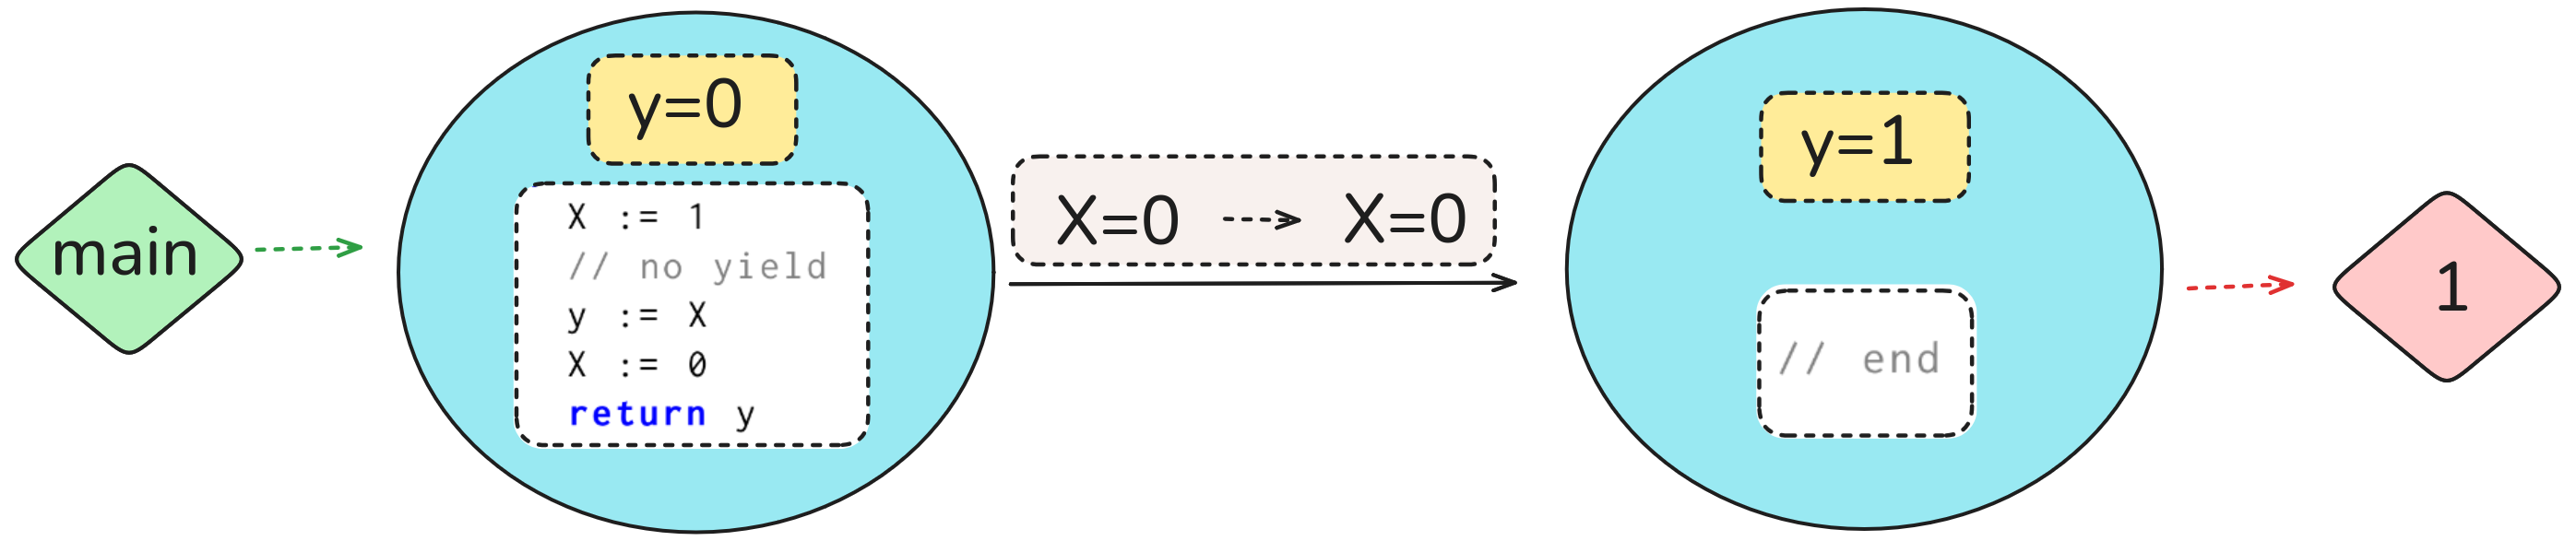
\includegraphics[width=0.9\textwidth]{plots/code_1_NS.png}
	\caption{Network System for interleaving executions of Listing~\ref{lst:MotivatingExample1Ser} program.}
	\label{fig:code1ExampleNS}
\end{figure}


\begin{figure}[H]
	\centering
	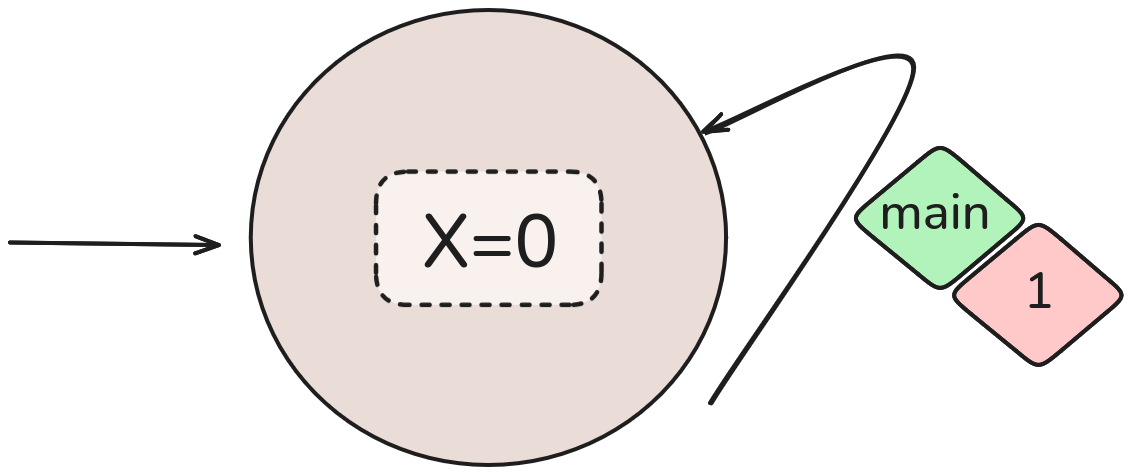
\includegraphics[width=0.35\textwidth]{plots/code_1_NFA.png}
	\caption{NFA for serialized executions of Listing~\ref{lst:MotivatingExample1Ser} program.}
	\label{fig:code1ExampleNFA}
\end{figure}



\begin{figure}[H]
	\centering
	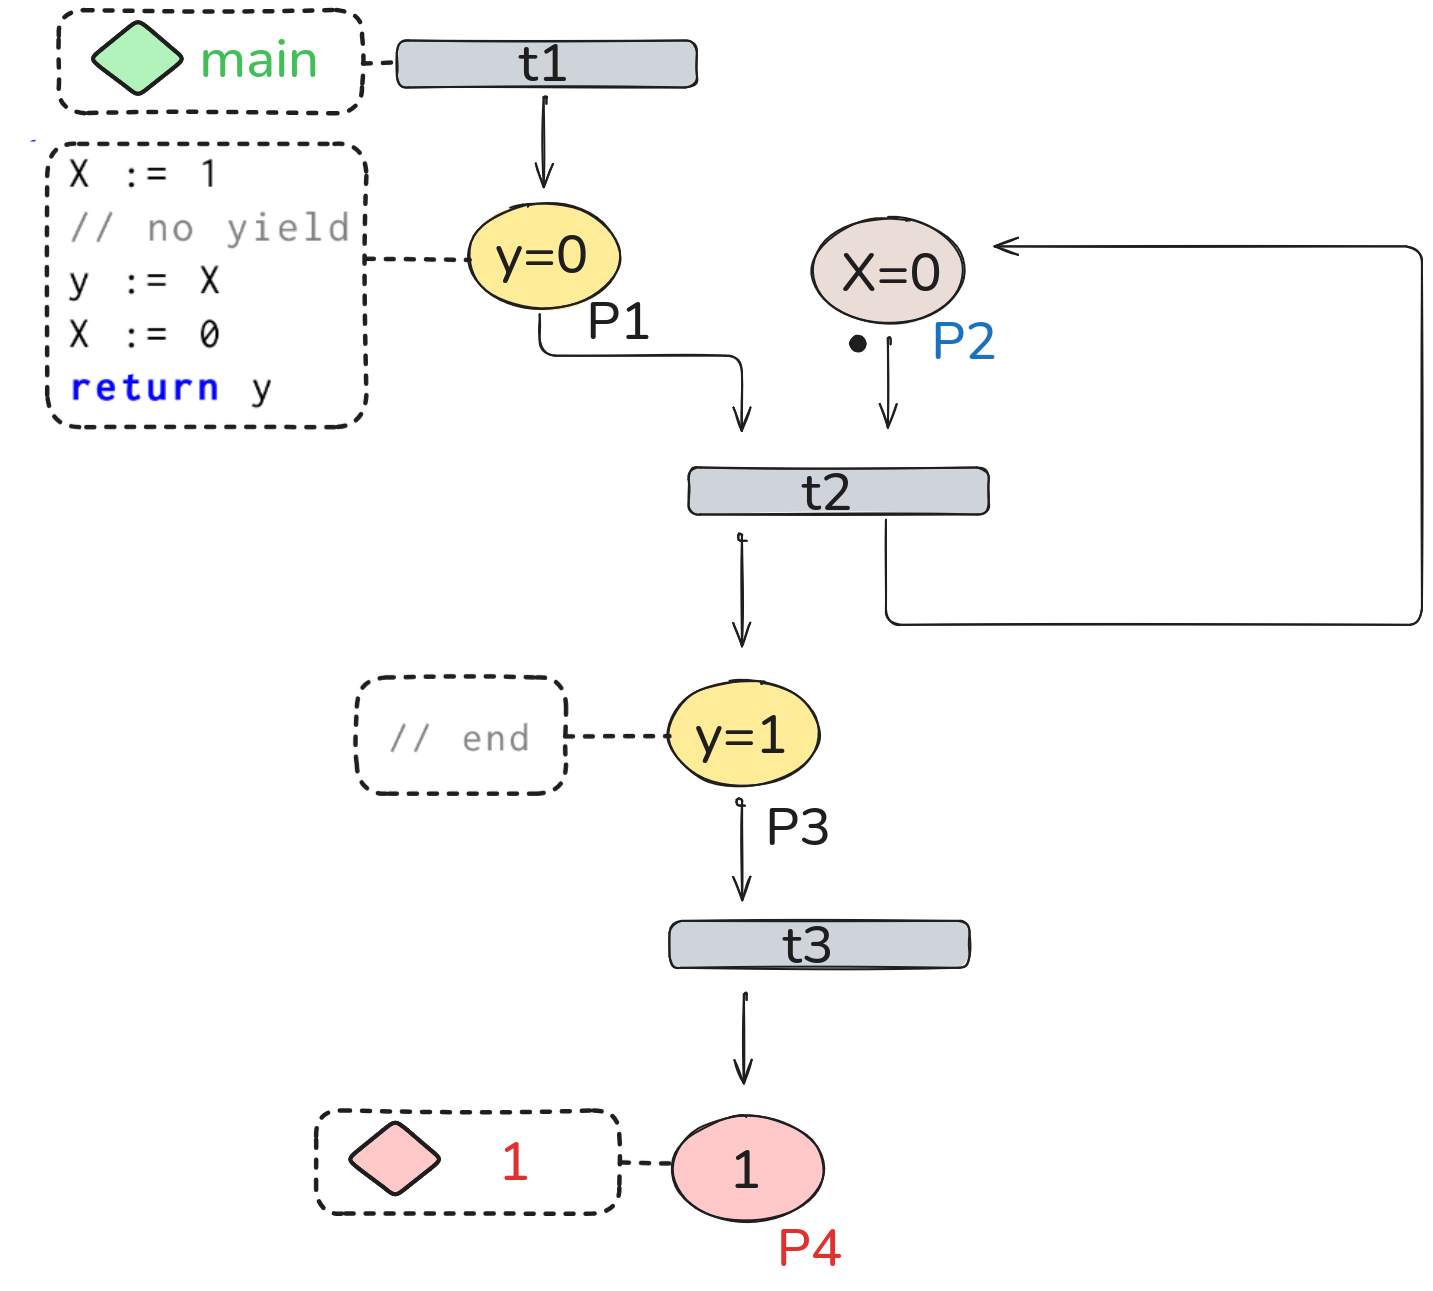
\includegraphics[width=0.6\textwidth]{plots/code_1_PN_with_annotation.png}
	\caption{Petri Net for interleaving executions of Listing~\ref{lst:MotivatingExample1Ser} program.}
	\label{fig:code1ExamplePN}
\end{figure}

%

\subsection{Motivating Examples \#2}
\label{appendix:subsec::Ex1B:NS}

For details, see the main text (Sec.~\ref{sec:problem-definition}).


\subsection{Motivating Examples \#3}
\label{appendix:subsec:Ex1C:NS}

Recall our third motivating example, presented in Listing~\ref{lst:MotivatingExample3Ser}.

\begin{minipage}[t]{0.3\textwidth}
	\begin{lstlisting}[caption={With yield and lock (serializable)}]
		request foo: 
			// lock
			while (L == 1): 
				yield
			L := 1 
		
			X := 1
			yield
			y := X 
			X := 0
		
			// unlock    
			L := 0
			return y 
	\end{lstlisting}
\end{minipage}

This program corresponds to the following Network System (NS):

\begin{figure}[htbp]
	\centering
	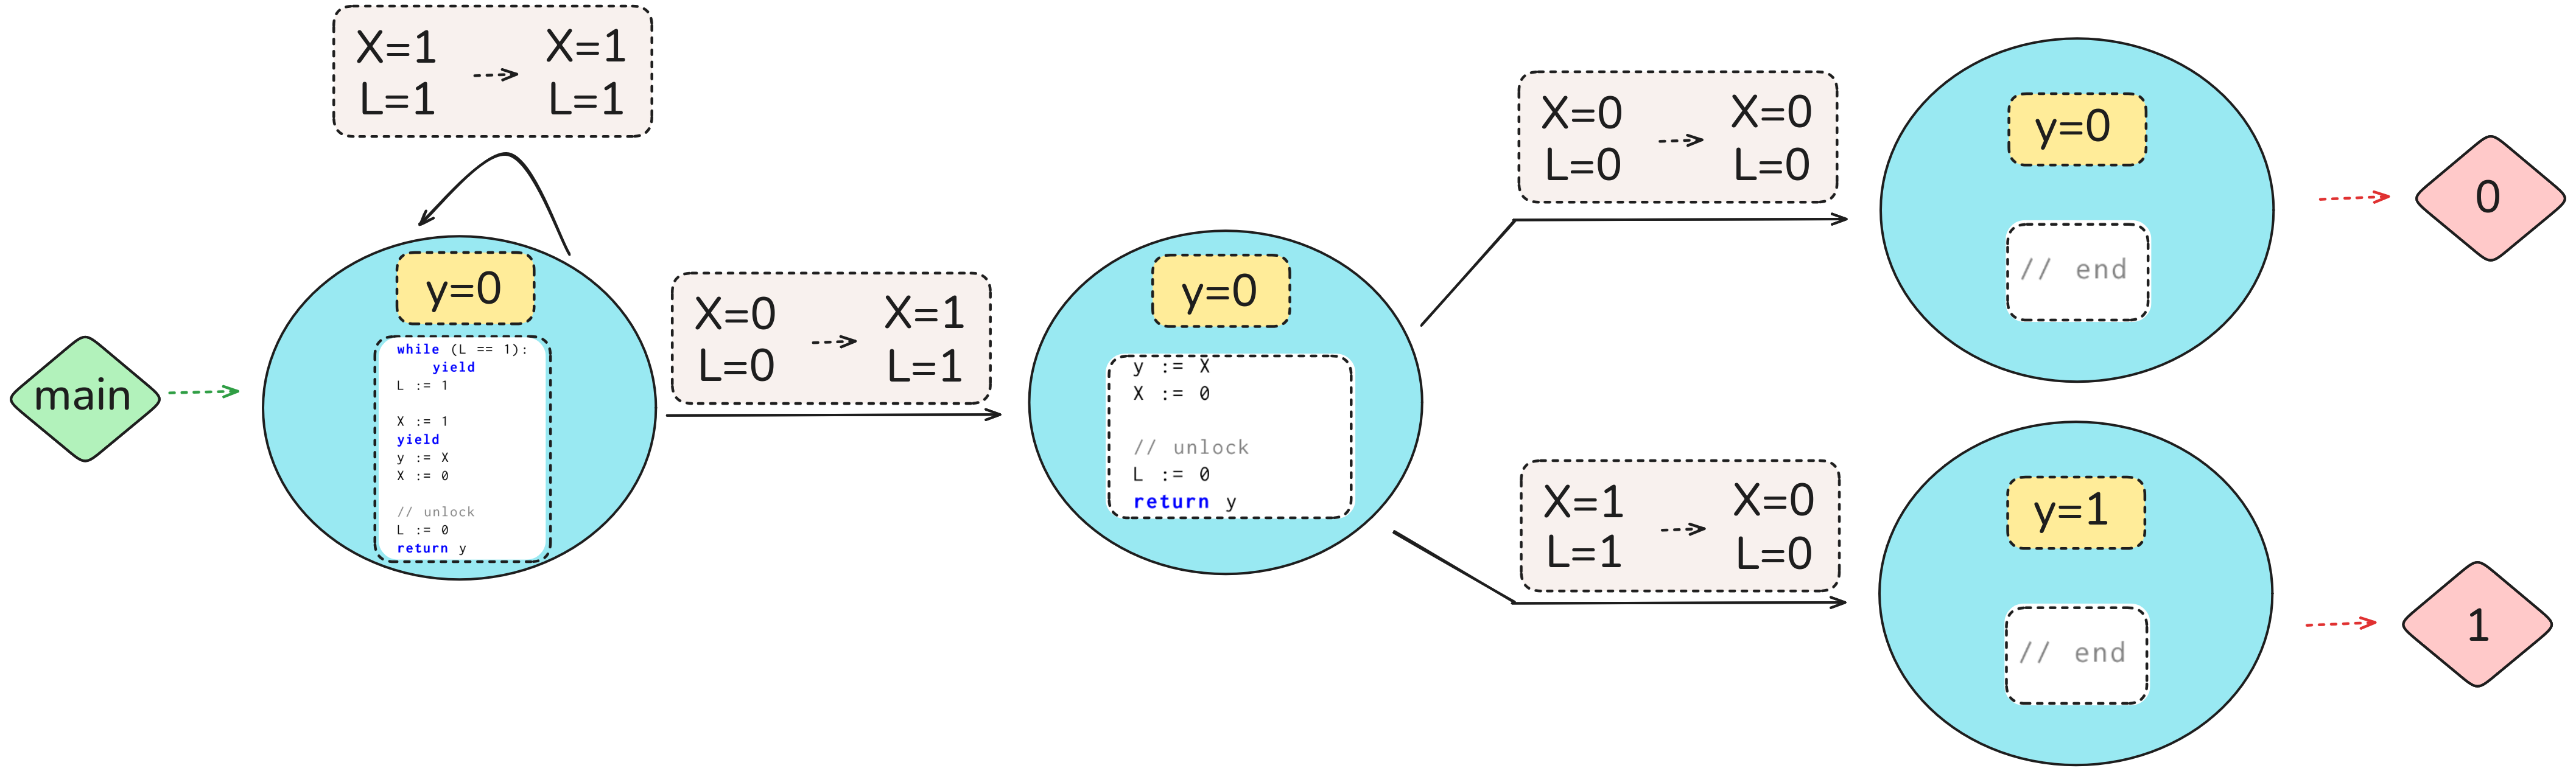
\includegraphics[width=1.1\textwidth]{plots/code_3_NS.png}
	\caption{Network System for interleaving executions of Listing~\ref{lst:MotivatingExample3Ser} program.}
	\label{fig:code3ExampleNS}
\end{figure}


\begin{figure}[htbp]
	\centering
	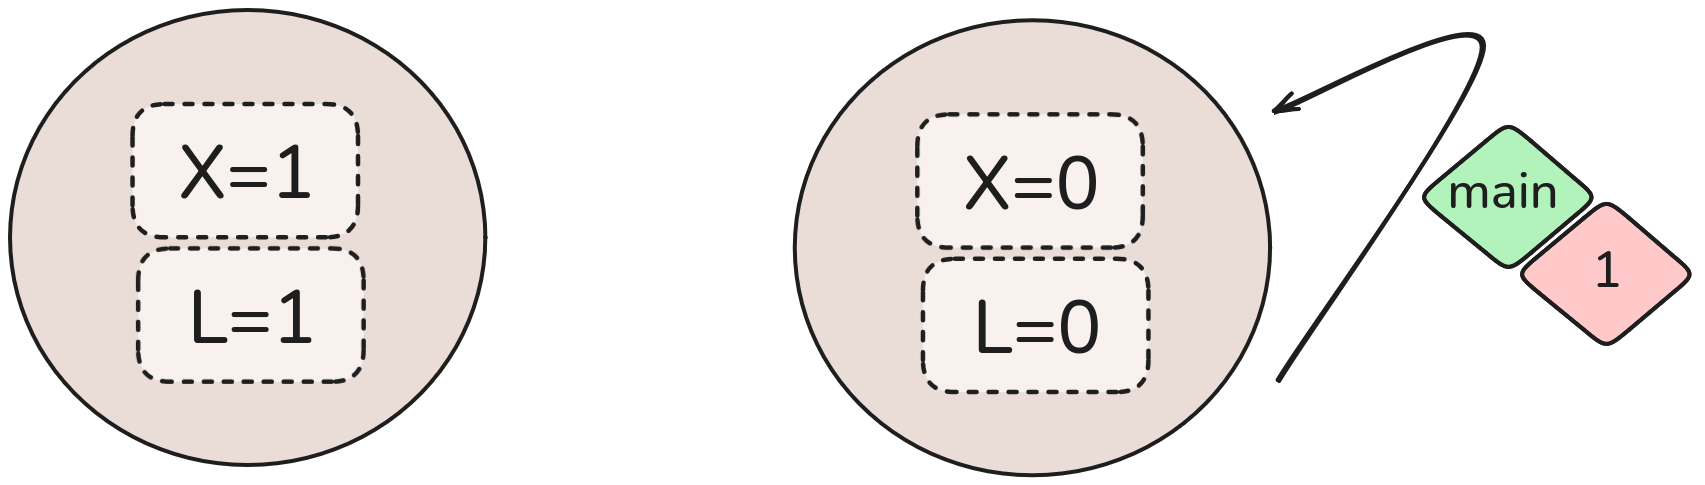
\includegraphics[width=0.4\textwidth]{plots/code_3_NFA.png}
	\caption{NFA for serialized executions of Listing~\ref{lst:MotivatingExample3Ser} program.}
	\label{fig:code3ExampleNFA}
\end{figure}



\begin{figure}[H]
	\centering
	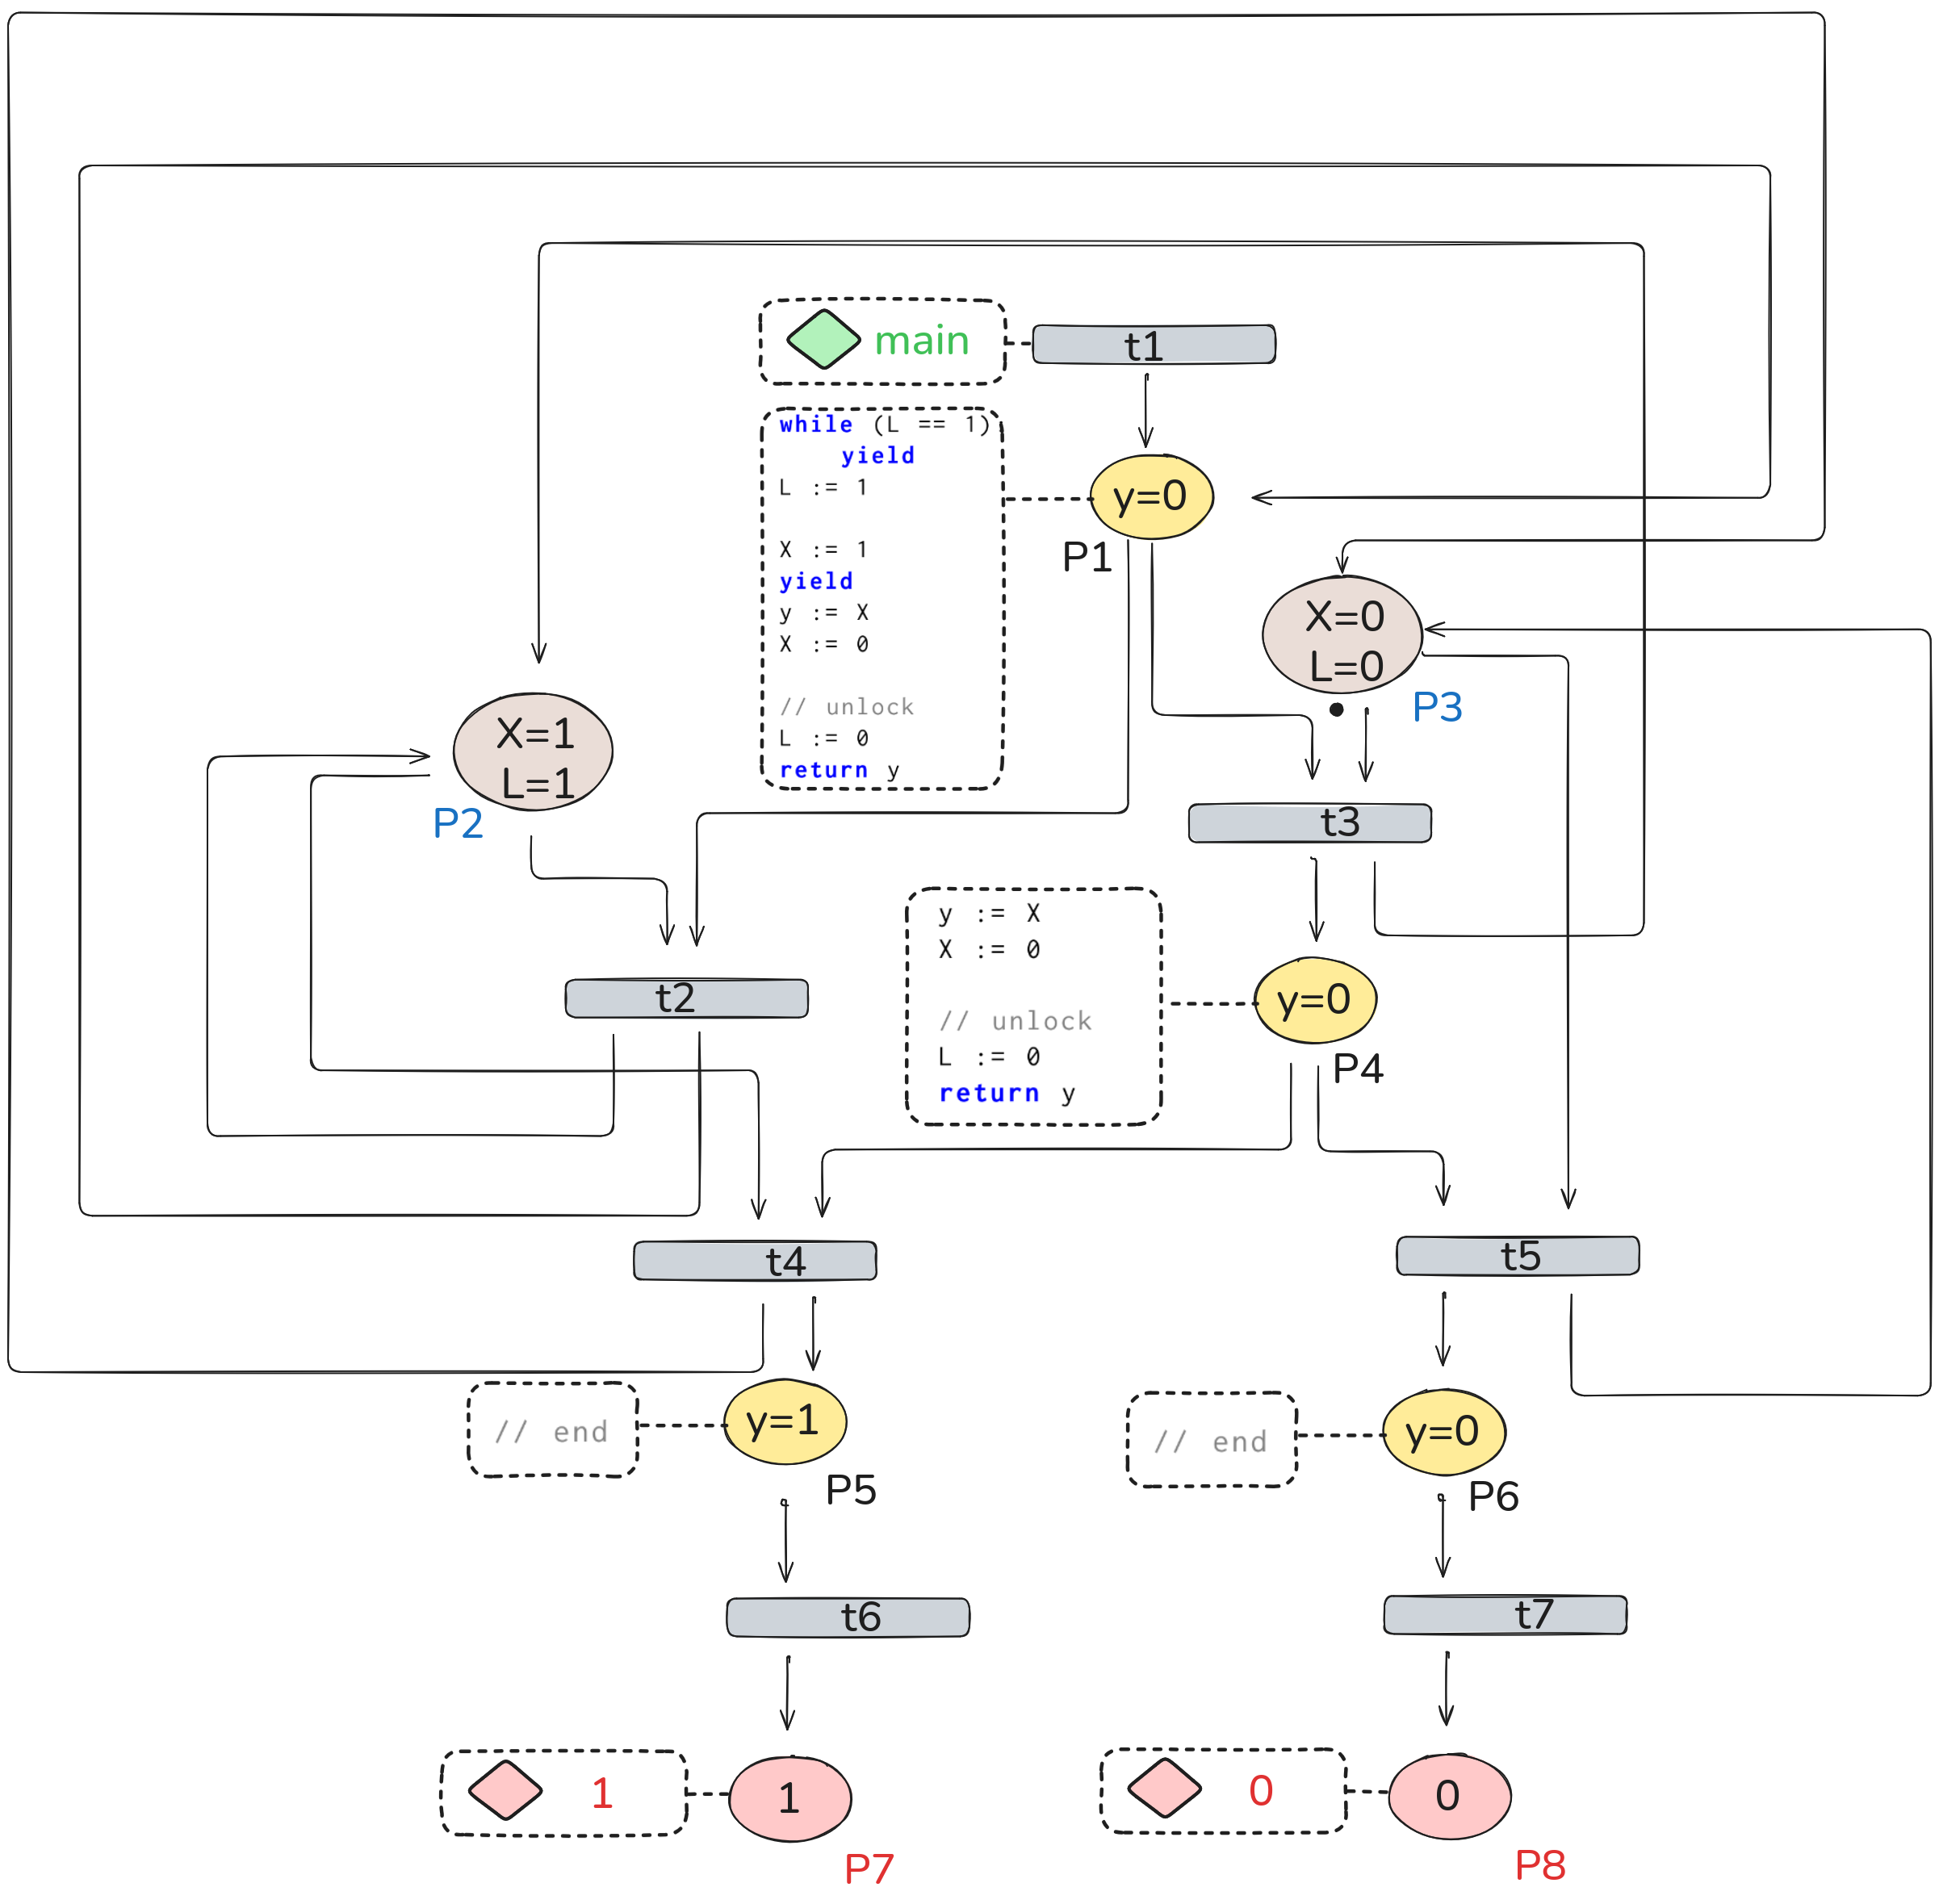
\includegraphics[width=0.8\textwidth]{plots/code_3_PN_with_annotation.png}
	\caption{Petri Net for interleaving executions of Listing~\ref{lst:MotivatingExample3Ser} program.}
	\label{fig:code3ExamplePN}
\end{figure}

\newpage
\appendix

\section{Motivating Example: Snapshot Isolation}
\label{appendix:snapshotIsolationExample}



The next program is motivated by system monitoring.
The system has two nodes (represented by the global variables $N_1$ and $N_2$) which monitor ongoing traffic in the network, and are originally both active, as indicated by their initial values [$N_1=1,N_2=1$].
%
The {\color{ForestGreen}$\blacklozenge_\text{main}$} request takes a ``snapshot'' of the system, i.e., locally records the current activation status of each of the two nodes.
%
Subsequently, in the first request, and any future ones in which both nodes are active, each in-flight request thread  non-deterministically decides which of the two nodes to deactivate, i.e. set [$N_i:=0$]. This policy is consistent with real-world settings for maintaining overall energy efficiency.
%
The {\color{ForestGreen}$\blacklozenge_\text{main}$} request eventually returns the current sum of active nodes in the system.
%
In order for the system to emulate multiple iterations, our setting also includes two additional requests, {\color{ForestGreen}$\blacklozenge_\text{activate\_n1}$},{\color{ForestGreen}$\blacklozenge_\text{activate\_n2}$} which activate nodes $N_1$ and $N_2$, respectively.
%
We note that the program is not serializable due to the yield operation that appears immediately after the recording (snapshot) of the node activity. One such example for a non-serializable behavior occurs when two {\color{ForestGreen}$\blacklozenge_\text{main}$} requests record two active monitor nodes and yield; Then, having each request turn off the complement node. As a result of each request operating based on its isolated ``snapshot'' of the initial global state, both monitor nodes can be turned off and we can attain a request with {\color{ForestGreen}$\blacklozenge_\text{main}$}/{\color{red}$\blacklozenge_0$} (for [$N_1+N_2=0+0=0$]).
%
We note that in any serializable execution, no two {\color{ForestGreen}$\blacklozenge_\text{main}$} requests can record both monitors as active, and hence, a response of {\color{red}$\blacklozenge_0$} is unattainable via serializable executions.




\begin{minipage}[t]{1.0\textwidth}
	\begin{lstlisting}[caption={Snapshot-based monitor deactivation (not serializable)}]
				// initialize both monitors to be active
				N_1_ACTIVE := 1
				N_2_ACTIVE := 1
				
				request main:
					// take snapshot
					n_1_active_snapshot := N_1_ACTIVE
					n_2_active_snapshot := N_2_ACTIVE
					yield
					
					if (n_1_active_snapshot == 1) and (n_2_active_snapshot == 1):
					// if both nodes active --- choose which one to deactivate 
						if (?): 
							  N_1_ACTIVE := 0
						else:
							  N_2_ACTIVE := 0
						
					return N_1_ACTIVE + N_2_ACTIVE  // total active nodes
					
				
				request activate_n1:
					    N_1_ACTIVE := 1
				
				request activate_n2:
					    N_2_ACTIVE := 1
				
				
			\end{lstlisting}
\end{minipage}

%only 0 in non-serializable runs!

%\todo{start}

%/snapshot_isolation_directly_as_NS_with_yields

%\begin{figure}[h]
%	\centering
%	\includegraphics[width=1.0\linewidth]{plots/snapshot\_isolation\_JSON\_with\_yields.pdf}
%	\caption{Snapshot Isolation with Yields.}
%	\label{fig:snapshotIsolationJsonWithYields}
%\end{figure}
%
%
%
%%/snapshot_isolation_directly_as_NS_without_yields
%
%\begin{figure}[h]
%	\centering
%	\includegraphics[width=1.0\linewidth]{plots/snapshot\_isolation\_JSON\_without\_yields.pdf}
%	\caption{Snapshot Isolation without Yields.}
%	\label{fig:snapshotIsolationJsonWithoutYields}
%\end{figure}


%\todo{maybe we have: (1) a copy of the global automaton; (2) a copy of the local automaton (with yields) with coloring of edges that don't exist in the one without yields}


%\begin{figure}[h]
%	\centering
%	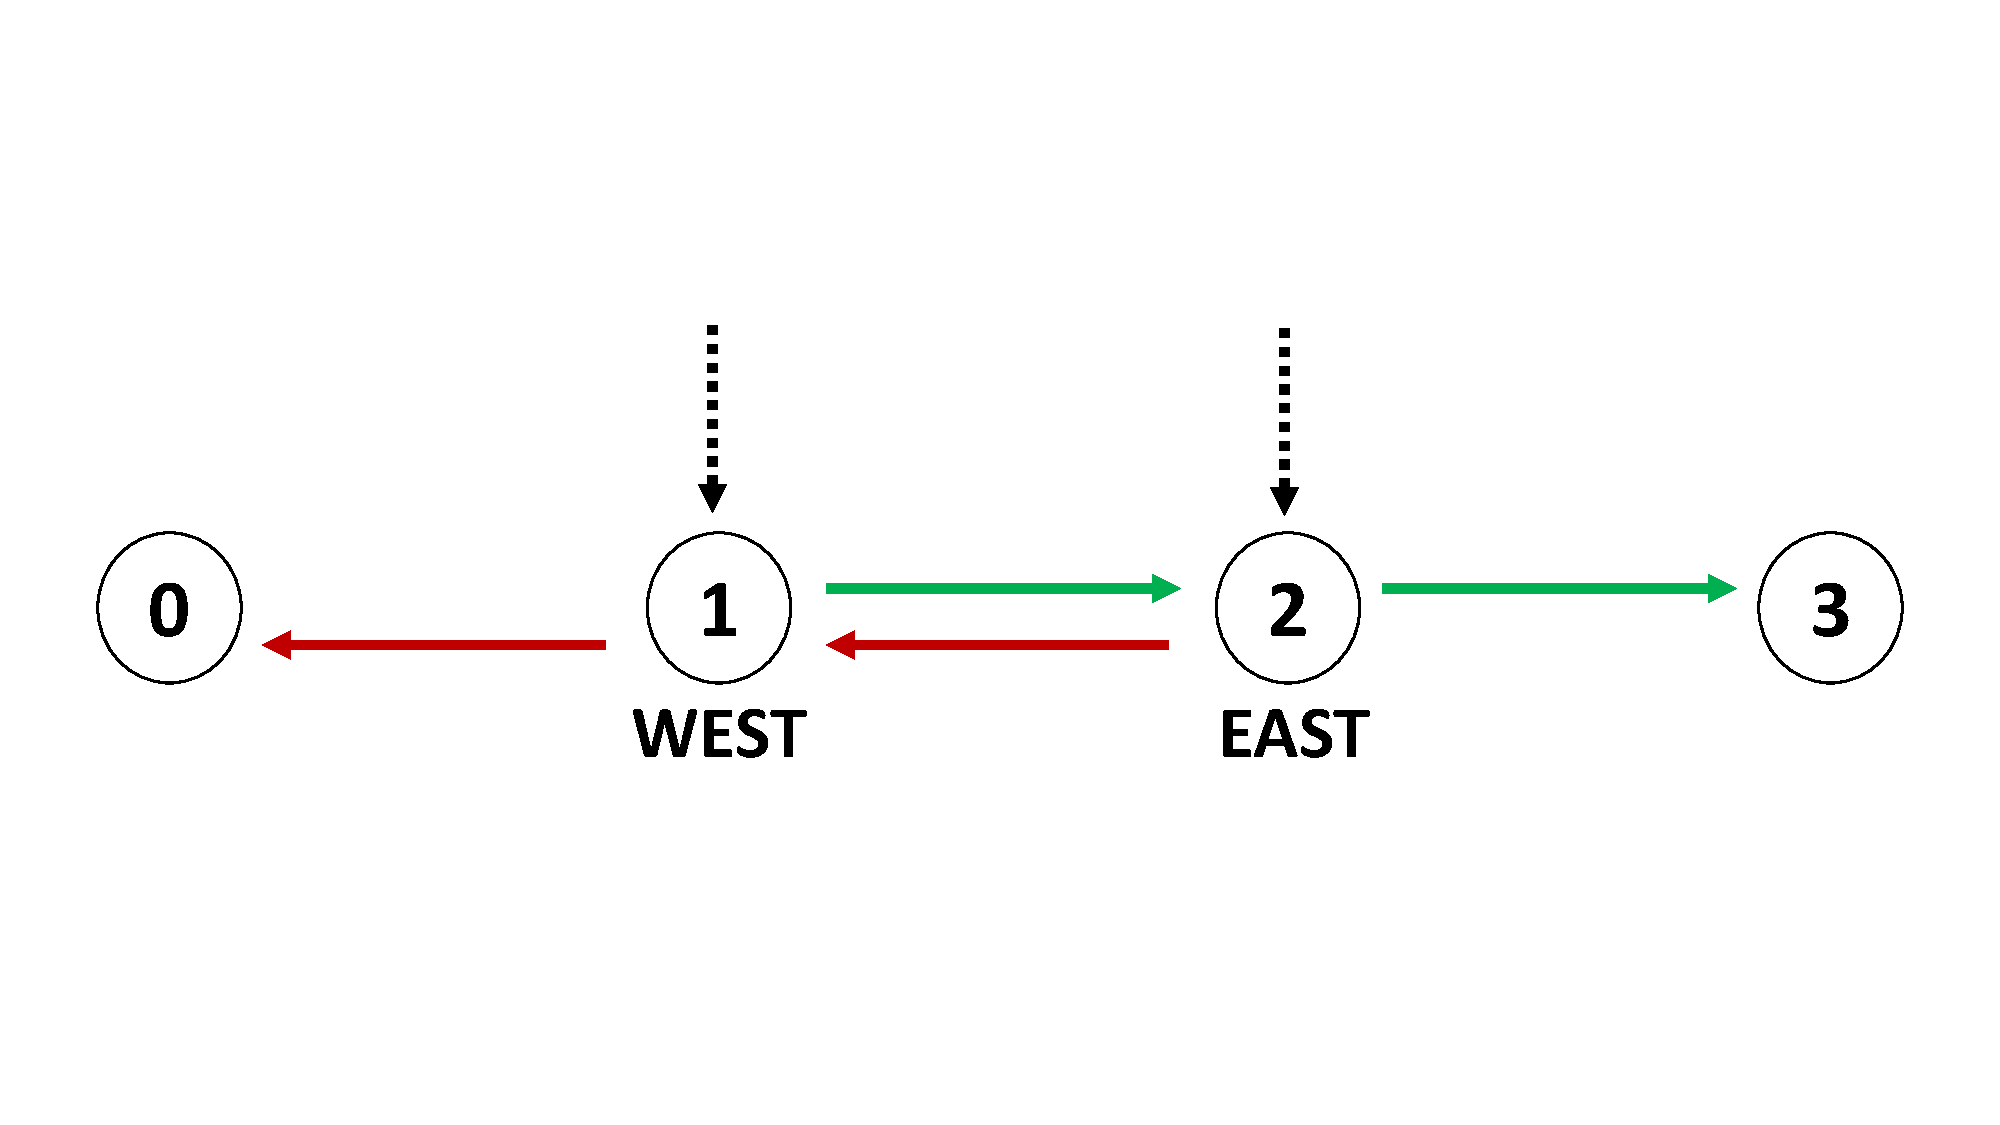
\includegraphics[width=0.65\linewidth]{plots/BgpColoredRouting.pdf}
%	\caption{Routing policy in example 7.}
%	\label{fig:pdfimage}
%\end{figure}

%\newpage
%
%
%example – 8
%
%\noindent
%\begin{minipage}[t]{0.45\textwidth}
%	\begin{lstlisting}[caption={foo (serializable)}]
	%	request foo: 
	%	    if (?):
	%	        X := (X + 2) % 3 
	%	        // no yield
	%	        return X
	%	
	%	    else:
	%	        X := (X + 1) % 3
	%	        // no yield
	%	        return X
	%		\end{lstlisting}
%\end{minipage}
%\hfill
%\begin{minipage}[t]{0.45\textwidth}
%\begin{lstlisting}[caption={foo (non serializable)}]
%request foo: 
%     if (?):
%         X := (X + 2) % 3 
%         yield
%         return X
%
%     else:
%         X := (X + 1) % 3
%         yield
%         return X
%	\end{lstlisting}
%\end{minipage}
%
%One output that is attainable only via non-serializable executions is 
%\[
%\{(foo,1),(foo,1),(foo,1),(foo,3)\}
%\]
%
%
%%\newpage
%
%
%example – 9
%
%\noindent
%\begin{minipage}[t]{0.45\textwidth}
%	\begin{lstlisting}[caption={foo (serializable)}]
%request foo:
%    if(STOP == 0):
%        X := (X + 1) % 4
%
%    yield
%
%    if(STOP == 0):
%        X := (X + 1) % 4
%
%        STOP := ?
%        
%        if(STOP == 1):
%	        return X
%        return 0
%	\end{lstlisting}
%\end{minipage}
%\hfill
%\begin{minipage}[t]{0.45\textwidth}
%	\begin{lstlisting}[caption={foo (non serializable)}]
%request foo:
%    if(STOP == 0):
%        X := (X + 1) % 4
%
%    yield
%
%    if(STOP == 0):
%        X := (X + 2) % 4
%
%        STOP := ?
%        
%        if(STOP == 1):
%	        return X
%        return 0
%	\end{lstlisting}
%\end{minipage}





\newpage
%% Appendix
%\appendix

\section{Proof: Bidirectional Optimization Correctness}
\label{appendix:BidirectionalProof}

\subsection{Preliminaries}

\begin{definition}[Petri Net]
	A \emph{Petri net} is a tuple
	\[
	N = (P,\,T,\,\Pre,\,\Post)
	\]
	where
	\begin{itemize}
		\item $P$ is a finite set of \emph{places},
		\item $T$ is a finite set of \emph{transitions},
		\item $\Pre: P\times T \to \mathbb{N}$ is the \emph{pre-incidence} function,
		\item $\Post: P\times T \to \mathbb{N}$ is the \emph{post-incidence} function.
	\end{itemize}
\end{definition}

\begin{definition}[Marking]
	A \emph{marking} is a function $M: P \to \mathbb{N}$. We write $M(p)$
	for the number of tokens in place $p$.  The initial marking is
	denoted $M_0$.  A transition $t\in T$ is \emph{enabled} at marking
	$M$ if $\forall p\in P:\,M(p)\ge\Pre(p,t)$.  Firing $t$ yields the
	new marking
	\[
	M' = M - \Pre(\cdot,t) + \Post(\cdot,t),
	\]
	written $M \xrightarrow{t} M'$.
\end{definition}

\begin{definition}[Firing Sequence]
	A sequence $\sigma = t_1 t_2 \cdots t_k \in T^*$ is \emph{fireable}
	from $M_0$ if there exist markings $M_1,\dots,M_k$ such that
	$M_0\xrightarrow{t_1}M_1\cdots\xrightarrow{t_k}M_k$.  We write
	$M_0 \xrightarrow{\sigma} M_k$.
\end{definition}

\begin{definition}[Semilinear Target Set]
	A \emph{semilinear} set $S\subseteq \mathbb{N}^P$ is a finite union of
	linear sets.  We assume $S$ is given by a finite description of its
	linear components.  We view $S$ as the \emph{target} set of markings
	we wish to reach.
\end{definition}

\subsection{The Bidirectional Pruning Algorithm}

Let $N=(P,T,\Pre,\Post)$, initial marking $M_0$, and target set
$S\subseteq\mathbb{N}^P$ be fixed.

\begin{definition}[Forward Over-Approximation]
	Define the operator $\mathcal{F}:\mathcal{P}(P\cup T)\to\mathcal{P}(P\cup T)$ by
	\[
	X \mapsto X
	~\cup~
	\{\,t\in T \mid \forall p\in P:\; \Pre(p,t)>0 \implies p\in X\}
	~\cup~
	\{\,p\in P \mid \exists t\in X\cap T,\ \Post(p,t)>0\}.
	\]
	Starting from $X_0 = \{\,p\mid M_0(p)>0\}$, iterate
	$X_{i+1} = \mathcal{F}(X_i)$ until a least fixed-point
	$X^*=\bigcup_i X_i$ is reached.  Call $X^*_P = X^*\cap P$ the set of
	\emph{forward-reachable} places.
\end{definition}

\begin{definition}[Backward Over-Approximation]
	Let
	\[
	Y_0 = \{\,p\in P \mid \exists M\in S:\;M(p)\neq0\}
	\]
	be the places unconstrained to zero by the target.  Define
	$\mathcal{B}:\mathcal{P}(P\cup T)\to\mathcal{P}(P\cup T)$ by
	\[
	Y \mapsto Y
	~\cup~
	\{\,t\in T \mid \forall p\in P:\; \Post(p,t)>0 \implies p\in Y\}
	~\cup~
	\{\,p\in P \mid \exists t\in Y\cap T,\ \Pre(p,t)>0\}.
	\]
	Iterate $Y_{i+1} = \mathcal{B}(Y_i)$ until a least fixed-point
	$Y^*=\bigcup_i Y_i$ is reached.  Call $Y^*_P = Y^*\cap P$ the set of
	\emph{backward-relevant} places.
\end{definition}

\begin{definition}[Pruned Net]
	The \emph{pruned} subnet is
	\[
	N' = \bigl(P',\,T',\,\Pre|_{P'\times T'},\,\Post|_{P'\times T'}\bigr)
	\]
	where
	\[
	P' = X^*_P \;\cap\; Y^*_P,
	\quad
	T' = \{\,t\in T \mid
	\forall p:\;\Pre(p,t)>0\implies p\in P',\;
	\forall p:\;\Post(p,t)>0\implies p\in P'
	\}.
	\]
\end{definition}

\subsection{Invariant and Correctness}

Intuitively, $P'$ contains exactly those places that
\emph{may} occur in some firing sequence from $M_0$ to a marking in $S$.

\begin{definition}[Witnessable Place]
	A place $p\in P$ is \emph{witnessable} if there exists a firing
	sequence $\sigma\in T^*$ and markings $M$ and $M'$ such that
	\[
	M_0 \xrightarrow{\sigma_1} M
	\quad\text{and}\quad
	M \xrightarrow{\sigma_2} M'
	\quad\text{with}\quad
	M(p)>0
	\quad\text{and}\quad
	M'\in S.
	\]
	In other words, $p$ can carry a token in some execution from $M_0$ into the target set $S$.
\end{definition}

\begin{theorem}[Pruning Invariant]
	\label{thm:invariant}
	If a place $p$ is witnessable, then $p\in P'$.  Equivalently, the
	pruned net $N'$ \emph{over-approximates} the set of witnessable places.
\end{theorem}

\begin{proof}
	We split the argument into two parts.
	
	\paragraph{(1) Forward-reachability.}
	Suppose $p$ is witnessable.  Then there is a prefix
	$\sigma_1\in T^*$ such that $M_0\xrightarrow{\sigma_1}M$ and
	$M(p)>0$.  By standard Petri-net monotonicity, every place that
	receives a token in the course of $\sigma_1$ must appear in the
	forward fixed-point $X^*_P$.  Hence $p\in X^*_P$.
	
	\paragraph{(2) Backward-relevance.}
	Again, since $p$ is witnessable, there is a suffix
	$\sigma_2\in T^*$ from $M$ to $M'\in S$ with $M(p)>0$.  Working
	backwards from $S$, every place that can contribute to satisfying
	semilinear constraints appears in the backward fixed-point $Y^*_P$.
	Thus $p\in Y^*_P$.
	
	\paragraph{Conclusion.}
	Combining (1) and (2) yields $p\in X^*_P\cap Y^*_P = P'$, as desired.
\end{proof}

\subsection{Termination and Complexity}

\begin{lemma}
	Each iteration of $\mathcal{F}$ and $\mathcal{B}$ strictly increases
	the set of included elements (unless already at the fixed-point), and
	the total number of elements is finite.  Hence both reach their
	fixed-points in at most $|P|+|T|$ iterations each.
\end{lemma}

\begin{proof}
	Immediate from monotonicity and finiteness.
\end{proof}

\noindent
Therefore the bidirectional pruning converges in polynomial time
(mostly linear in the net-size per pass), and preserves exactly the
places and transitions that \emph{may} appear in some execution from
$M_0$ into $S$.

%\newpage

\section{Proof of Inductive Invariant}
\label{appendix:InductiveInvariantExample}


\begin{proof}
	
Define the predicate
\[
\begin{aligned}
	I(P_{1},\dots,P_{8})
	:={}&
		(P_{1},\textcolor{black}{P_{2}},\textcolor{black}{P_{3}},P_{4},P_{5},P_{6},\textcolor{black}{P_{7}},\textcolor{black}{P_{8}})
		\;\mapsto\;\\
		&\quad
		\exists\,e_{0},\dots,e_{5}\ge0.\;
		\Bigl(
		e_{2}-e_{1}+\textcolor{black}{P_{3}}-1=0\;\land\;
		e_{2}+P_{1}-e_{5}=0\;\land\;
		P_{5}-e_{1}+e_{4}=0\;\land\\
		&\qquad\quad
		-\,e_{4}+\textcolor{black}{P_{7}}=0\;\land\;
		P_{6}+e_{3}-e_{0}=0\;\land\;
		\textcolor{black}{P_{8}}-e_{3}=0\;\land\\
		&\qquad\quad
		-\,e_{2}+e_{1}+e_{0}+P_{4}=0\;\land\;
		-\,e_{2}+e_{1}+\textcolor{black}{P_{2}}=0
		\Bigr)
		\;\land\;
		\bigl(P_{4}-1\ge0\;\lor\;\textcolor{black}{P_{3}}-1\ge0\bigr).
	\end{aligned}
	\]
	
	
	\medskip\noindent
	\textbf{(1) Initialization.}
	The initial marking has $P_{3}=1$ and $P_{1}=P_{2}=P_{4}=P_{5}=P_{6}=P_{7}=P_{8}=0$.
	Choose $e_{0}=\cdots=e_{5}=0$.  Then
	\[
	e_{i}\ge0,\quad
	e_{2}-e_{1}+P_{3}-1=0-0+1-1=0,\;\dots,\;-e_{2}+e_{1}+P_{2}=0,
	\]
	and 
	\[
	P_{4}-1\ge0\;\lor\;P_{3}-1\ge0
	\;=\;-1\ge0\;\lor\;0\ge0
	\;=\;\texttt{FALSE}\;\lor\;\texttt{TRUE}
	\;=\;\texttt{TRUE}.
	\]
	Thus $I$ holds initially.
	
	\medskip\noindent
	\textbf{(2) Consecution.}
	One checks for each transition $t_{k}$ of the Petri net that
	\[
	I(M)\;\Longrightarrow\;I\bigl(t_{k}(M)\bigr).
	\]
	In each case the same $(e_{0},\dots,e_{5})$ can be adjusted (per the SMT certificate) to show the eight equalities and the disjunction remain valid. See our accompanying artifact~\cite{ArtifactRepository} for generating a full proof in the standard \texttt{SMT-LIB} format.
	
	\medskip\noindent
	\textbf{(3) Refutation of the property.}
	Suppose by contradiction that both $I(P)$ and it holds that:
	\[
	\phi(P):\quad
	P_{1}=0,\;
	P_{2}\ge0,\;
	P_{3}\ge0,\;
	P_{4}=0,\;
	P_{5}=0,\;
	P_{6}=0,\;
	P_{7}=0,\;
	P_{8}\ge1.
	\] 
	
	\noindent
	From
	\[
	e_{2}-e_{1}+P_{3}-1=0
	\quad\text{and}\quad
	-e_{2}+e_{1}+P_{2}=0
	\]
	we get
	\[
	P_{2}=1-P_{3}.
	\]
	From
	\[
	P_{8}-e_{3}=0
	\quad\text{and}\quad
	P_{6}+e_{3}-e_{0}=0
	\]
	and from the assumption that $P_6=0$, we get
	\[
	e_{0}=e_{3}=P_{8}
	\].
	
	
	\noindent
	Similarly, the invariant equalities 
	$(-\,e_{2}+e_{1}+e_{0}+P_{4}=0)$ and $(	-\,e_{2}+e_{1}+\textcolor{black}{P_{2}}=0)$
	induce
	\[
	P_{2}=P_{4}+e_{0}=P_{4}+P_{8},
	\]
	thus
	\[
	P_{8}=P_2-P4=(1-P_{3})-P_{4}=1-P_{3}-0=1-P_3.
	\]
	as we also assume that $P_4=0$.


	
	
	\noindent
	But $\phi$ also gives $P_{3}\ge0$ and $P_{8}\ge1$, hence $P_{3}=0$.  
	Furthermore, as our invariant includes a conjunction with $\bigl(P_{4}-1\ge0\;\lor\;\textcolor{black}{P_{3}}-1\ge0\bigr)$. As we assume by negation that the semilinear set is reachable, then $P_4=0$; and in order for both the invariant and the property to hold, then necessarily $P_3 \ge 1$, in contradiction with $P_3=0$.
	%
	  Thus $I\land\phi$ is unsatisfiable, i.e., 
	%\[
	$
	I(P)\;\Longrightarrow\;\neg\phi(P)$
	.
	%\]
	This completes the proof that $I$ is an inductive invariant refuting the given property.
\end{proof}


%\newpage


\section{Toy Petri Net Example}
\label{appendix:toyPN}

Observe the toy Petri Net in Fig.~\ref{fig:toyPN}.

\begin{figure}[H]
	\centering
	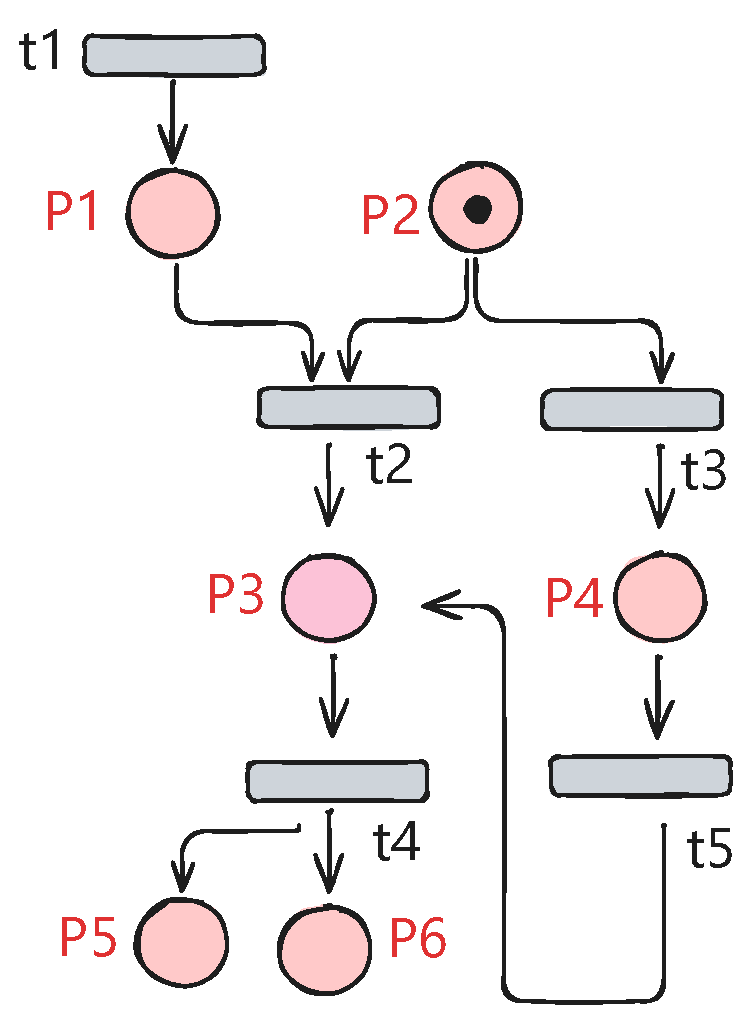
\includegraphics[width=0.3\textwidth]{plots/toy_PN_example.pdf}
	\caption{A toy Petri Net.}
	\label{fig:toyPN}
\end{figure}



We formally define the net as follows:

 \(N=(P,T,\mathsf{pre},\mathsf{post},M_0)\) with
\[
P=\{P_1,P_2,P_3,P_4,P_5,P_6\},\quad
T=\{t_1,t_2,t_3,t_4,t_5\},
\]
and pre/post given by
\[
\begin{array}{c|cccccc}
	& P_1 & P_2 & P_3 & P_4 & P_5 & P_6 \\ \hline
	\mathsf{pre}(t_1)  & 0 & 0 & 0 & 0 & 0 & 0 \\
	\mathsf{post}(t_1) & 1 & 0 & 0 & 0 & 0 & 0 \\ \hline
	\mathsf{pre}(t_2)  & 1 & 1 & 0 & 0 & 0 & 0 \\
	\mathsf{post}(t_2) & 0 & 0 & 1 & 0 & 0 & 0 \\ \hline
	\mathsf{pre}(t_3)  & 0 & 1 & 0 & 0 & 0 & 0 \\
	\mathsf{post}(t_3) & 0 & 0 & 0 & 1 & 0 & 0 \\ \hline
	\mathsf{pre}(t_4)  & 0 & 0 & 1 & 0 & 0 & 0 \\
	\mathsf{post}(t_4) & 0 & 0 & 0 & 0 & 1 & 1 \\ \hline
	\mathsf{pre}(t_5)  & 0 & 0 & 0 & 1 & 0 & 0 \\
	\mathsf{post}(t_5) & 0 & 0 & 1 & 0 & 0 & 0
\end{array}
\]
The initial marking is
\[
M_0 = (0,1,0,0,0,0)^\top 
\]

Differently put, there is a single token in place $P_2$.


\begin{itemize}
	\item A \emph{reachable} final marking is
	\[
	M_f = (0,0,0,0,1,1)^\top,
	\]
	reached by the firing sequence
	\[
	M_0 \xrightarrow{t_1} M_1
	\xrightarrow{t_2} M_2
	\xrightarrow{t_4} M_f,
	\]
	where
	\[
	M_1 = (1,1,0,0,0,0)^\top,
	\quad
	M_2 = (0,0,1,0,0,0)^\top.
	\]
	\item A \emph{non‐reachable} marking is
	\[
	M_{nr} = (0,1,1,0,0,0)^\top,
	\]
	since producing a token at \(P_3\) (via \(t_2\)) necessarily consumes the only token in \(P_2\), and no transition replenishes \(P_2\), hence it is impossible for these two places to hold a single token in any reachable firing. We note the if the initial marking was 
	
	\[
	M_f = (0,2,0,0,0,0)^\top,
	\]
	then such a marking would have been reachable, by firing a single transition $t_2$.
\end{itemize}






\newpage


\section{SMPT}
\label{appendix:smpt}



\texttt{SMPT} (\emph{Satisfiability Modulo Petri Net}) is a tool incorporating a portfolio of symbolic model checking techniques --- including Bounded Model Checking (BMC)~\cite{BiCiClZh99}, state equation reasoning~\cite{Mu77}, $k$-induction~\cite{ShSiSt20}, Property Directed Reachability (PDR)~\cite{Br11,AmDaHu22}, and random state space exploration. It acts as a front-end to an SMT solver (\texttt{z3}~\cite{DeBj08} in our setting), while also incorporating domain-specific knowledge from Petri net theory, such as invariants and structural properties. \texttt{SMPT} has participated in the last five editions of the \textit{Model Checking Contest} (MCC), an international competition for model checking tools. In its most recent participation, it achieved a bronze medal and a $100\%$ confidence level score, meaning it never returned an incorrect verdict~\cite{mcc:2025}.

\texttt{SMPT} distinguishes itself from other tools in two ways that are particularly relevant to our setting and motivated its adoption. First, to the best of our knowledge, it is the only model checker for Petri nets that provides a proof of its verdict, regardless of the underlying verification technique. This means it either produces a witness trace when the property is reachable, or, more interestingly, a certificate of non-reachability~\cite{AmDaHu22} when the property is not reachable.
%
The second distinguishing feature relates to ongoing work. \texttt{SMPT} supports polyhedral reductions~\cite{AmBeDa21}, as elaborated in Sec.~\ref{sec:discussion}.



%\newpage

\end{document}
